\documentclass[12pt]{article}

% ---------------------------------------------------------------------------
% Estimation and Inference on Two-Threshold Value Functionals -- VERSION 6
% ---------------------------------------------------------------------------
% Standalone-compilable companion to may_2026.tex ("Inference on Policy Value
% under Admissibility-Constrained Optimal Treatment Rules").  Designed to slot
% in as the "Estimation and Inference of the Value Functional" section of the
% JMP: it generalizes Chen, Chen & Gao (2025) [single threshold: plug-in,
% analytical variance, sieve-Riesz inference] and the extended draft
% [quadratic debiasing, sieve DML] to value functionals defined by TWO
% thresholds, and develops the combined (doubly debiased) procedure left open
% in Remark 7 of the extended draft.  Macros match may_2026.tex.
%
% v6 changes (see "Revision note (v6)" after the abstract):
%   * adds the missing empirical score-stability condition for variance
%   * defines the DML norms, projection, fold convention, and growing-sieve regime
%   * imposes composite-score equivalence and Lyapunov conditions for DD
%   * makes corner noncancellation optional rather than globally maintained
%   * corrects the remaining LOO arm weights and DD order overclaims
%   * restricts support-edge and mesh-resonance statements to justified cases
% ---------------------------------------------------------------------------

\usepackage[margin=1in]{geometry}
\usepackage{setspace}
\usepackage{amsmath,amssymb,amsthm,mathtools,bm}
\usepackage{enumitem}
\usepackage{natbib}
\usepackage[colorlinks=true,linkcolor=blue,citecolor=blue,urlcolor=blue]{hyperref}
\usepackage{booktabs}
\usepackage{longtable}
\usepackage{graphicx}
\usepackage[expansion=false]{microtype}% bbm fonts are non-scalable
\usepackage{bbm}
\usepackage{array}

\onehalfspacing

\newtheorem{theorem}{Theorem}[section]
\newtheorem{proposition}[theorem]{Proposition}
\newtheorem{lemma}[theorem]{Lemma}
\newtheorem{corollary}[theorem]{Corollary}
\newtheorem{assumption}[theorem]{Assumption}
\newtheorem{definition}[theorem]{Definition}
\newtheorem{remark}[theorem]{Remark}
\newtheorem{example}[theorem]{Example}

\newcommand{\R}{\mathbb{R}}
\newcommand{\E}{\mathbb{E}}
\newcommand{\Prob}{\mathbb{P}}
\newcommand{\1}{\mathbbm{1}}
\newcommand{\dd}{\,\mathrm{d}}
\newcommand{\Haus}{\mathcal{H}}
\newcommand{\norm}[1]{\left\lVert #1 \right\rVert}
\newcommand{\abs}[1]{\left\lvert #1 \right\rvert}
\newcommand{\inner}[2]{\left\langle #1, #2 \right\rangle}
\newcommand{\argmax}{\operatorname*{arg\,max}}
\newcommand{\Th}{\Theta}
\newcommand{\Mg}{\mathcal{M}_{g}}
\newcommand{\Mh}{\mathcal{M}_{h}}
\newcommand{\Corner}{\mathcal{C}}
\newcommand{\Ng}{\norm{\nabla g_{0}}}
\newcommand{\Nh}{\norm{\nabla h_{0}}}

\title{Estimation and Inference on Two-Threshold Value Functionals\thanks{%
This section extends the single-threshold framework of \citet{ccg2025} and its
debiased-estimation companion to value functionals defined by the intersection
of two estimated decision boundaries. It is written to be self-contained;
notation follows the JMP draft \texttt{may\_2026.tex}.}}
\author{Zhenxiao Chen\thanks{Department of Economics, University of
Pennsylvania, USA, zxchen@upenn.edu.}}
\date{\today\\[4pt]\normalsize Version 6}

\begin{document}
\maketitle

\begin{abstract}
\noindent We study estimation and inference for value functionals of the form
$\Th_{0}=\E\big[\1\{g_{0}(X)\geq0\}\,\1\{h_{0}(X)\geq0\}\,v_{0}(X)\big]$,
where $g_{0}$ and $h_{0}$ are two nonparametric contrast functions estimated
from the same experiment. Such \emph{two-threshold} functionals arise whenever
a planner imposes a pointwise admissibility screen on top of a benefit margin:
leading examples are the share of the population that benefits in the short
run but is harmed in the long run under a surrogate-index treatment rule
\citep{acik2024}, and treatment-path welfare components
of an optimal dynamic regime.

Our primary contribution is the \emph{second-order} shape calculus of such
functionals, which we derive in full and verify numerically. The first
shape derivative is a sum of two boundary (Hausdorff) integrals over the
two margins. The second contains, in addition to two margin curvature forms,
a codimension-two \emph{corner} integral over
$\{g_{0}=0\}\cap\{h_{0}=0\}$ together with two corner \emph{diagonal} terms
weighted by the cosine of the intersection angle. We then give a complete
order accounting of the terms this generates in a sieve plug-in expansion:
the corner contributes $O(K_{n}/n)$, the margins $O(K_{n}^{1+1/d}/n)$, and
we show that the margin bound can be attained in suitably phased
mesh-resonant examples, while its exact order for a fixed general geometry
remains open. The accounting implies
that margin-by-margin quadratic debiasing \`{a} la \citet{cg2026} leaves a
corner cross term whose upper bound is rate-relevant on the window
$(d+1)/2<s\leq d-1$, nonempty for $d\geq4$; matching relevance requires the
stated optional noncancellation condition. We therefore construct
corner-aware split-sample and
leave-one-out corrections, with a tuning-free half-sample jackknife
representation.

The inferential results are stated as \emph{conditional} theorems and we are
explicit about what is and is not proved. Under estimator-specific
third-order and series-linearization remainder conditions that we do not
derive from primitive smoothness assumptions, the corner-aware split-sample
estimator attains $n^{-s/(2s+1)}$ under $s>(d+1)/2$; this threshold controls
the displayed leading terms but is not, by itself, a primitive sufficient
condition for those remainders.
A centered normal limit requires strict
undersmoothing and, for the plug-in, strict $s>d$; we give the explicit
sieve-dimension windows. We also correct an error in the previous version's
\emph{doubly debiased} estimator, which combined the quadratic correction
with a cross-fitted Riesz correction: as constructed there, the Riesz score
reintroduces exactly the own-half second-order diagonals the quadratic
correction removes. We derive the score of the composite split-sample
functional, which is $D\Th(\bar\gamma)-\tfrac12D\Th(\hat\gamma^{A})$ rather
than $\tfrac12D\Th(\hat\gamma^{A})$, and give a three-fold construction that
repairs it. Monte Carlo experiments calibrated to the \citet{banerjee2015}
graduation experiment, following the Wasserstein-GAN calibration protocol of
\citet{cr2023}, illustrate the corner mechanism; their doubly debiased cells
evaluate the superseded construction and we read them accordingly.
\end{abstract}

\paragraph{Status of the results.} Theorem~\ref{thm:D2} (the second shape
derivative), Proposition~\ref{prop:D1}, the polarization identity
\eqref{eq:polar-limit}, the transversal smooth-face support-edge term of
Remark~\ref{rem:edge}, and
the jackknife finite-difference identity of Lemma~\ref{lem:jackknife} are
established, and verified numerically to ten significant digits
(Appendix~\ref{app:numeric}). The order accounting of
Section~\ref{sec:orders} is a set of \emph{upper bounds} whose exponent
arithmetic we have checked symbolically; Remark~\ref{rem:cancel} identifies
where those bounds are and are not attained. Theorems~\ref{thm:plugin},
\ref{thm:ss}, \ref{thm:dml} and~\ref{thm:dd} are \emph{conditional}: each
displays, in one place, every remainder condition it uses ---
Assumption~\ref{ass:rem} collects the main Taylor, empirical-process, moment,
and series-linearization conditions, while Assumption~\ref{ass:path} collects
the additional jackknife conditions --- and
Appendix~\ref{app:proofs}, \S B.4 lists exactly which of those we have not
verified from primitive conditions. The reader should treat the four
theorems as specifications of what must be proved, complete as to their
hypotheses but not as to their proofs. In particular, Version~4's proposed
$C^{1}$ modulus for $\gamma\mapsto D^{2}\Th(\gamma)$ was not merely
unproved: it is false because $D^{2}\Th$ depends on the curvature of
$\gamma$. Version~5 therefore imposes the two actual evaluation-point
remainders directly and gives a $C^{2}$ modulus only as an optional
sufficient condition.

A drafting convention that matters for reading Section~\ref{sec:quad}: we
distinguish throughout between the \emph{ideal} split-sample estimators,
built from the closed-form $D^{2}\Th$ of Theorem~\ref{thm:D2}, and their
\emph{feasible} finite-difference (jackknife) counterparts. The
decomposition identities hold exactly \emph{within} each family and only up
to a fourth-order error \emph{across} them; v3 conflated the two.

\paragraph{Revision note (v6).} This version repairs the inferential gaps
left in v5. \emph{(i)} In-sample variance consistency now requires empirical
stability of the estimated representer against the true residuals; population
$sd$-norm convergence alone is not used as an empirical LLN. \emph{(ii)} The
DML product norms, projection, evaluation-fold convention, and
$K_n\to\infty$ regime are defined explicitly. \emph{(iii)} The DD theorem
requires the sum of the two composite representers to approach the ordinary
representer and imposes a conditional Lyapunov condition for the actual
fold score; equality of variances is no longer treated as a CLT.
\emph{(iv)} The empirical-measure component of the composite functional is
evaluated on the held-out fold and expanded rather than called ``common.''
\emph{(v)} Corner noncancellation is optional and invoked only for matching
lower bounds. \emph{(vi)} The remaining common-weight LOO formula and
unjustified DD $\asymp$ statements are corrected. \emph{(vii)} The
support-edge formula is restricted to transversal intersections with smooth
support faces, and the mesh-resonance calculations are described as
finite-sample evidence rather than asymptotic lower bounds.

\paragraph{Revision note (v5).} This version corrects nine remaining
defects in v4. \emph{(i)} The $C^{1}$ second-derivative modulus is replaced by
direct, estimator-specific remainder conditions. A $C^{2}$ modulus is stated
only as a sufficient condition, because curvature is not continuous in the
$C^{1}$ topology. \emph{(ii)} The fourth-derivative condition for the
jackknife is retained as an explicit high-level assumption; spline degree
ensures existence but does not make its constant uniform in $K_{n}$.
\emph{(iii)} Ratio consistency of the Riesz variance now requires
\emph{Riesz-weighted} residual consistency, not merely an unweighted
$L^{2}$ condition. \emph{(iv)} The stochastic expansions are written as
arm-wise sums, consistently with the four regressions actually estimated.
\emph{(v)} The corrected DD theorem is studentized by the variance of its
actual composite score; no unproved equivalence with the ordinary two-band
score is used. \emph{(vi)} The exact corner centering identity is stated only
for the oracle derivative statistic; evaluation at the estimated midpoint
and the jackknife each carry an explicit remainder. \emph{(vii)} Stale
$\asymp$, ``negligible,'' and cross-reference claims are corrected.
\emph{(viii)} The population-Gram series expansion now includes the
empirical-LS remainder instead of being written as an exact identity.
\emph{(ix)} Joint residual nondegeneracy and the moment condition needed for
variance ratio consistency are imposed explicitly.

\paragraph{Revision note (v4).} This version repairs internal defects of v3
that were mathematical, not merely unproved. \emph{(i)} v3 asserted
$\hat\Th_{SS}=\hat\Th_{SS}^{\mathrm{mar}}-\widehat{\mathrm{corner}}$ with
$\hat\Th_{SS}$ the ideal derivative-based estimator. That is false: the
polarization identity holds exactly for the \emph{jackknife} family, and
across families there is a fourth-order gap. Section~\ref{sec:quad} now
carries both families with their own exact identities
(\eqref{eq:polar-ideal} and \eqref{eq:polar-jack}).
\emph{(ii)} Theorem~\ref{thm:plugin}(i) controlled only the linear and
quadratic terms while the expansion contains a third-order remainder;
Assumption~\ref{ass:rem} now collects every remainder condition used
anywhere in the paper, and each theorem cites it.
\emph{(iii)} The jackknife centred CLT needs its own sieve window
$a<3d/(4d+7)$, not merely the smoothness condition \eqref{eq:jackcond};
Theorem~\ref{thm:ss}(iii) supplies it.
\emph{(iv)} The second-moment ``exact sandwich'' of v3 was written for a
single contrast regression; the paper's estimator runs \emph{four separate
arm regressions}, so the exact expression is an arm-wise sum of sandwiches
\eqref{eq:sandwich}, the localization error is additive rather than
relative, and the $h_{0}=-\tau_{Y}$ convention flips a sign.
\emph{(v)} Assumption~\ref{ass:dml}(c) claimed Hausdorff-distance plus
region-measure convergence was ``equivalent'' to normal-graph convergence.
It is not --- a surface can be Hausdorff-close while oscillating, with
divergent surface measure --- so (c) now \emph{requires} a normal-graph
representation with $C^{1}$ control, plus a convention for empty margins.
\emph{(vi)} The SS expansion also carries an evaluation-point remainder
$\{D^{2}\Th(\bar\gamma)-D^{2}\Th(\gamma_{0})\}[\Delta,\Delta]$, distinct from
the Taylor remainder; both are now controlled by a single
\emph{second-derivative modulus} condition. Version~5 replaces that invalid
$C^{1}$ modulus by direct conditions on both actual remainders; see
Assumption~\ref{ass:rem}(a).
\emph{(vii)} v3's proof of Theorem~\ref{thm:ss} justified variance
consistency by claiming the correction is $o_{p}(\mathrm{se})$. In the SS
smoothness window it need not be; consistency follows instead from the
asymptotically linear representation.
\emph{(viii)} The corner noncancellation condition was imposed on population
coefficients, which does not prevent the spline-weighted sequence from
cancelling; it is now imposed on the actual normalized sequence
$\tfrac{n}{K_{n}}\mathcal B_{\Corner,n}$, and the full-bracket and
cross-term conditions are stated separately, since neither implies the other.
\emph{(ix)} We add a condition that no earlier version or critique
identified: in the empirical-measure case the plug-in carries a
\emph{stochastic-equicontinuity} term $\tfrac1{\sqrt n}\mathbb G_{n}
[m_{\hat\gamma}-m_{\gamma_{0}}]$ of order $(K_{n}/n)^{3/4}$, which imposes
$a<d/(3d-2)$ and binds for $d\geq3$ (Remark~\ref{rem:equicont}).
\emph{(x)} Assorted repairs: uniform overlap; the stacked standard-deviation
norm defined on the summed influence rather than as a scalar; the bilinear
extension of $D^{2}\Th$ stated by polarization; ``shape (G\^ateaux)
derivative'' replacing ``pathwise derivative''; arm-residual consistency
added to Proposition~\ref{prop:var}; the composite representer conditions
and the empirical-measure fold convention added to Section~\ref{sec:dd};
$\asymp$ demoted to $O$ in Proposition~\ref{prop:margins}; the LOO claim
softened; and the internal contradiction between the abstract, the main
text, and Appendix~B.1 over mesh resonance resolved in favour of the
upper-bound reading.

Relative to v1--v2 the corrections recorded in the v3 note stand: the
invalidity of the old doubly debiased estimator and its composite-score
repair, the separation of rate statements from centred CLTs, the
margin/corner order distinction, and the two incorrect claims of
Remarks~\ref{rem:ls} and~\ref{rem:outofspan}. The Monte Carlo tables are
reproduced unchanged from v1; Section~\ref{sec:limits} states what they do
and do not support.

\section{Setup and Examples}\label{sec:setup}

\subsection{Data and estimands}

The observed data are an i.i.d.\ sample
$\{Z_{i}=(X_{i},W_{i},S_{i},Y_{i})\}_{i=1}^{n}$, where $X_{i}\in\mathcal
X\subset\R^{d}$ are covariates with density $f_{0}$ on a bounded rectangular
support, $W_{i}\in\{0,1\}$ is a binary treatment with
$(S_{i}(0),S_{i}(1),Y_{i}(0),Y_{i}(1))\perp W_{i}\mid X_{i}$ and overlap
$p_{0}(x):=\E[W_{i}\mid X_{i}=x]\in(0,1)$, $S_{i}$ is a short-run outcome
(or surrogate), and $Y_{i}$ is a long-run outcome. Define the arm means and
contrasts
\begin{align}
\mu_{S,0}(x,w):=\E[S_{i}\mid X_{i}=x,W_{i}=w], \qquad
\tau_{S}(x):=\mu_{S,0}(x,1)-\mu_{S,0}(x,0), \label{eq:tauS}\\
\mu_{Y,0}(x,w):=\E[Y_{i}\mid X_{i}=x,W_{i}=w], \qquad
\tau_{Y}(x):=\mu_{Y,0}(x,1)-\mu_{Y,0}(x,0). \label{eq:tauY}
\end{align}
Throughout we write $\gamma_{0}:=(g_{0},h_{0})$ for a generic pair of
identified contrast functions built from
$(\mu_{S,0},\mu_{Y,0})$ --- in the leading example $g_{0}=\tau_{S}$ and
$h_{0}=-\tau_{Y}$ --- and consider the \emph{two-threshold value functional}
\begin{equation}
\Th(\gamma_{0})
:=\int_{\mathcal X}\1\{g_{0}(x)\geq0\}\,\1\{h_{0}(x)\geq0\}\,
v_{0}(x)\,f(x)\dd x,
\label{eq:Theta}
\end{equation}
where $v_{0}$ is a known, user-chosen value weight and $f$ is the covariate
density of the target population. As in the single-threshold analysis we
distinguish the \emph{known-density} case ($f$ given, integral computed
numerically) and the \emph{empirical} case ($f=f_{0}$ unknown, integral
replaced by the sample average $n^{-1}\sum_{i}\1\{\cdot\}v_{0}(X_{i})$); the
first-order asymptotic theory is identical in both, because the additional
sampling error of the empirical measure is $O_{p}(n^{-1/2})$, which is
negligible relative to the slower boundary-driven rate of \eqref{eq:Theta}.
It is \emph{not} negligible at the sample sizes of Section~\ref{sec:mc}, and
we therefore carry it explicitly in the variance formula
\eqref{eq:two-band-var} below.

\subsection{Leading examples}

\begin{example}[Surrogate-induced harm share]\label{ex:harm}
A planner who observes only the short-run outcome adopts the surrogate-index
rule ``treat iff $\tau_{S}(x)\geq0$.'' The long-run criterion would instead
require $\tau_{Y}(x)\geq0$. With $g_{0}=\tau_{S}$, $h_{0}=-\tau_{Y}$, and
$v_{0}\equiv1$, \eqref{eq:Theta} becomes
\[
\theta_{0}=\Prob_{f}\big(\tau_{S}(X)\geq 0,\ \tau_{Y}(X)\leq 0\big),
\]
the mass of the population that the surrogate rule treats but that is harmed
in the long run --- a direct diagnostic of the surrogate-index approach of
\citet{acik2024}. This is the functional we take to the
calibrated Monte Carlo of Section~\ref{sec:mc}.
\end{example}

\begin{example}[Admissibility-constrained policy value]\label{ex:admiss}
In the two-item-checklist planner problem of the JMP draft, a hard
admissibility screen $g_{0}(x)\geq0$ (e.g.\ no expected severe side effect)
is imposed before the benefit margin $h_{0}(x)\geq0$; treated-population
aggregates take the form \eqref{eq:Theta} with $v_{0}$ equal to a utility,
cost, or eligibility weight.
\end{example}

\begin{example}[Dynamic treatment-path welfare]\label{ex:dtr}
The $(1,1)$ path-welfare component of an optimal two-stage dynamic regime,
$V_{11}^{*}=\E[Y^{(1,1)}\1\{\kappa(S)\geq0\}\1\{\delta(X^{(1)})\geq0\}]$,
has the same two-threshold structure, with the additional complication that
the first-stage contrast $\kappa$ is itself a functional of the second-stage
threshold. The static analysis of this section is the template for that case;
the extra ``moving-boundary-within-a-moving-boundary'' terms are treated in
the DTR section of the draft.
\end{example}

\subsection{Geometry and maintained assumptions}

Write $w(x):=v_{0}(x)f(x)$ for the boundary weight, and define the two
\emph{margins} and the \emph{corner}
\begin{align}
\Mg&:=\{x:g_{0}(x)=0,\ h_{0}(x)>0\},\qquad
\Mh:=\{x:h_{0}(x)=0,\ g_{0}(x)>0\},\nonumber\\
\Corner&:=\{x:g_{0}(x)=h_{0}(x)=0\}.
\label{eq:margins}
\end{align}

\begin{assumption}[Model]\label{ass:model}
(a) $\{Z_{i}\}$ is i.i.d.; $\mathcal X$ is bounded rectangular; and overlap
is \emph{uniform}, $p_{0}(x)\in[\underline p,1-\underline p]$ for some
$\underline p>0$ --- pointwise $p_{0}(x)\in(0,1)$ does not suffice, because
the inverse-propensity weights of \eqref{eq:aggmoments} and the arm-wise
Gram matrices $R_{w}$ of \eqref{eq:sandwich} must be bounded uniformly;
(b) $\mu_{S,0}(\cdot,w),\mu_{Y,0}(\cdot,w)\in\Lambda^{s}(\mathcal X)$ (H\"older
class) with $s>1$, for $w\in\{0,1\}$; (c) the conditional second moments
$\sigma_{S}^{2}(x,w),\sigma_{Y}^{2}(x,w)$ of the regression residuals
$\epsilon_{S,i}:=S_{i}-\mu_{S,0}(X_{i},W_{i})$,
$\epsilon_{Y,i}:=Y_{i}-\mu_{Y,0}(X_{i},W_{i})$ are bounded and bounded away
from zero, and the conditional covariance matrix of
$(\epsilon_{S,i},\epsilon_{Y,i})$ has eigenvalues bounded above and bounded
away from zero uniformly in $(x,w)$. In particular, the conditional correlation
$\rho_{SY}(x,w):=\mathrm{Corr}(\epsilon_{S,i},\epsilon_{Y,i}\mid
X_{i}=x,W_{i}=w)$ is well defined and uniformly bounded away from $\pm1$.
Moreover,
$\E[\abs{\epsilon_{o,i}}^{2+\varsigma}\mid X_{i},W_{i}]$ is bounded for some
$\varsigma>0$ and $o\in\{S,Y\}$;
(d) $v_{0}$ is bounded and continuously
differentiable, and $f$ is bounded with bounded gradient, absolutely
continuous w.r.t.\ $f_{0}$ with bounded Radon--Nikodym derivative bounded away
from zero on a neighborhood of $\Mg\cup\Mh$.
\end{assumption}

\begin{assumption}[Regular margins and transversal corner]\label{ass:geometry}
$g_{0}$ and $h_{0}$ are twice continuously differentiable in neighborhoods of
$\{g_{0}=0\}$ and $\{h_{0}=0\}$ respectively, with
(a) $\Ng\geq\underline c>0$ on $\{g_{0}=0\}$ and
$\Nh\geq\underline c>0$ on $\{h_{0}=0\}$;
(b) (\emph{transversality}) on $\Corner$, the angle $\omega(x)$ between
$\nabla g_{0}(x)$ and $\nabla h_{0}(x)$, defined by $\cos\omega(x)
=\inner{\nabla g_{0}}{\nabla h_{0}}/(\Ng\Nh)$,
satisfies $\abs{\sin\omega(x)}\geq\underline c_{T}>0$;
(c) $\Haus^{d-1}(\Mg)+\Haus^{d-1}(\Mh)<\infty$ and
$\Haus^{d-2}(\Corner)<\infty$;
(d) (\emph{no support edge}) the level sets $\{g_{0}=0\}$ and $\{h_{0}=0\}$
meet $\partial\mathcal X$ only where $w$ vanishes, so that no margin
terminates at the edge of the covariate support and the boundary calculus
below involves only the margins and their common corner.
\end{assumption}

Under Assumption~\ref{ass:geometry}, the closures of $\Mg$ and $\Mh$ in the
interior of $\mathcal X$ are $(d-1)$-dimensional $C^{2}$
submanifolds-with-boundary whose common relative boundary is the
$(d-2)$-dimensional corner $\Corner$ (a finite set of points
when $d=2$; empty when $d=1$ or when the constraints never bind jointly).
Transversality rules out tangential intersections, at which the corner would
inflate to a higher-dimensional set and the second-order calculus below would
fail.

We separate the core nondegeneracy condition from an optional corner
noncancellation condition because two-sided statements are false without the
relevant restriction: a functional with $v_{0}\equiv0$ or empty margins has
no boundary irregularity, while a signed corner coefficient can cancel even
when a corner exists.

\begin{assumption}[Parameter space and nondegeneracy]\label{ass:nondegen}
(a) (\emph{Parameter space.}) $\Lambda^{s}_{c}(\mathcal X)$ denotes the ball
of radius $c$ in the H\"older space of order $s$ on $\mathcal X$, and the
statistical model is
\begin{align*}
\mathcal P^{s}_{c}:=\Big\{P:\ &\mu_{S,0}(\cdot,w),\mu_{Y,0}(\cdot,w)
\in\Lambda^{s}_{c}\ \text{for }w\in\{0,1\},\ \text{and }P\text{ satisfies}\\
&\text{Assumptions~\ref{ass:model}--\ref{ass:geometry} and (b) below
with common constants}\Big\}.
\end{align*}
Rates and minimax statements are uniform over $\mathcal P^{s}_{c}$.
(b) (\emph{Nonvanishing boundary weight.})
\[
\Haus^{d-1}(\Mg)\vee\Haus^{d-1}(\Mh)\;\geq\;\underline m>0
\qquad\text{and}\qquad
\inf_{\Mg\cup\Mh}w\;\geq\;\underline w>0 .
\]
At least \emph{one} margin must be nondegenerate; this is what makes
$\Th_{0}$ irregular and, with the upper bound
$\Haus^{d-1}(\Mg)+\Haus^{d-1}(\Mh)<\infty$ of
Assumption~\ref{ass:geometry}(c), delivers $\sigma_{n}^{2}\asymp
K_{n}^{1/d}$. Without it the representer norm can be $O(1)$ and $\Th_{0}$ is
$\sqrt n$-estimable. It is deliberately ``$\vee$'' and not ``$\wedge$'': the
single-threshold submodel used for the minimax lower bound in
Theorem~\ref{thm:plugin}(ii) has $\Mh=\emptyset$, and requiring both margins
to be nondegenerate would exclude it from $\mathcal P^{s}_{c}$ and break the
nesting argument.
\end{assumption}

\begin{assumption}[Optional corner noncancellation]\label{ass:cornernc}
Let
$\mathcal B_{\Corner,n}$ and $\mathcal B^{\times}_{\Corner,n}$ denote,
respectively, the full corner coefficient \eqref{eq:corner-coef} and its
cross-term component \eqref{eq:corner-cross} defined in
Section~\ref{sec:orders}; both are deterministic sequences depending on the
sieve through the normalized second-moment functions
$\mathcal V_{\bullet,n}/K_{n}$. When $\Corner\neq\emptyset$, either of the
following may be imposed separately:
\begin{equation}
\text{(c1)}\quad
\liminf_{n}\Big|\frac{n}{K_{n}}\,\mathcal B_{\Corner,n}\Big|>0,
\qquad
\text{(c2)}\quad
\liminf_{n}\Big|\frac{n}{K_{n}}\,\mathcal B^{\times}_{\Corner,n}\Big|>0 .
\label{eq:noncancel}
\end{equation}
(c1) is used for lower bounds on the plug-in's corner bias, (c2) for the bias
that survives margins-only debiasing (Proposition~\ref{prop:margins}).
\emph{Neither implies the other}, and neither follows from pointwise
nonvanishing of $\varrho_{gh}$: the bracket in \eqref{eq:corner-coef} is
signed, its three components may offset, contributions from different corner
points may offset, and the spline-dependent weights
$\mathcal V_{\bullet,n}(x)/K_{n}$ vary across corner points and with $n$.
Each is needed only for its corresponding lower bound; no upper bound below
uses either.
If $\Corner=\emptyset$, neither condition is invoked and both corner
coefficients are identically zero.
\end{assumption}

\begin{remark}[$\Corner$ is not automatically material]\label{rem:cornerzero}
Assumption~\ref{ass:cornernc} is a genuine optional restriction, not a
formality. It is not part of $\mathcal P_c^s$ and is invoked only when a
matching corner lower bound is claimed.
At an orthogonal corner ($\cos\omega=0$) with $\rho_{SY}=0$ the bracket
vanishes identically; with $d=2$ and several corner points the terms carry
the sign of $\cos\omega$ at each point, which typically varies; and even with
a fixed nonzero pointwise coefficient the $n$-dependent weights could conspire
to cancel along a subsequence, which is why \eqref{eq:noncancel} is imposed
on the normalized sequence rather than on population quantities. In the
calibrated design of Section~\ref{sec:mc} the ten corners do not cancel
(Table~\ref{tab:anatomy}), but this is a property of that design.
\end{remark}

\begin{assumption}[Remainders]\label{ass:rem}
Write $\bar\Delta$ for a generic first-stage error, $\eta$ for a generic
direction, and $\mathrm{se}_{n}:=\sqrt{K_{n}^{1/d}/n}$.
\begin{enumerate}[leftmargin=2.2em,label=(\alph*)]
\item (\emph{Taylor and evaluation-point remainders.}) With
$R_{3}:=\tfrac12\{D^{2}\Th(\gamma_{\xi})
-D^{2}\Th(\gamma_{0})\}[\bar\Delta,\bar\Delta]$ the exact mean-value
remainder of the second-order expansion \eqref{eq:expansion}, and
$R_{3}^{SS}$ the total remainder of the corrected estimator defined in
\eqref{eq:R3SS}, the relevant one is $O_{p}(r_{n}^{*})$ where a rate is
claimed and $o_{p}(\mathrm{se}_{n})$ where a centred limit is claimed.
This is a direct, estimator-specific condition; no continuity of
$D^{2}\Th$ in the $C^{1}$ topology is presumed.
\item (\emph{Stochastic equicontinuity; empirical-measure case only.})
With $m_{\gamma}(x):=\1\{g(x)\geq0\}\1\{h(x)\geq0\}v_{0}(x)$,
\begin{equation}
n^{-1/2}\,\big|\mathbb G_{n}\big[m_{\hat\gamma}-m_{\gamma_{0}}\big]\big|
=o_{p}(\mathrm{se}_{n})
\quad\text{for centered limits},
\qquad
\mathbb G_{n}:=\sqrt n\,(\mathbb P_{n}-P).
\label{eq:equicont}
\end{equation}
For rate statements the corresponding requirement is
$n^{-1/2}|\mathbb G_n[m_{\hat\gamma}-m_{\gamma_0}]|
=O_p(r_n^*)$.
\item (\emph{Lyapunov.}) For some $\varsigma>0$,
$n^{-\varsigma/2}\E\big[\abs{v^{*}_{S}\epsilon_{S}+v^{*}_{Y}\epsilon_{Y}}
^{2+\varsigma}\big]/\sigma_{n}^{2+\varsigma}\to0$.
\item (\emph{Series linearization; sieve results only.}) For every full- and
split-sample series fit, the population-Gram expansion
\eqref{eq:decomp} has remainders $(r_g,r_h)$. After these are substituted in
the relevant linear, margin, corner, and finite-difference expressions, their
total contribution is $O_p(r_n^*)$ for a rate statement and
$o_p(\mathrm{se}_n)$ for a centered limit. The corresponding second-moment
remainders in \eqref{eq:corner-coef} are smaller than the displayed leading
orders. This condition is imposed directly; an empirical least-squares
coefficient does not equal its population-Gram linearization identically.
\end{enumerate}
\end{assumption}

Collecting the remainder conditions in one place is deliberate. Every
theorem below cites Assumption~\ref{ass:rem} explicitly, so that no
statement silently omits a term of its own expansion --- a defect of v3's
Theorem~\ref{thm:plugin}(i), which controlled the linear and quadratic terms
of \eqref{eq:expansion} but not $R_{3}$.

\begin{remark}[Why the remainder is imposed directly]\label{rem:c2modulus}
Version~4 tried to deduce Assumption~\ref{ass:rem}(a) from
\[
\big|\{D^{2}\Th(\gamma)-D^{2}\Th(\gamma_{0})\}[\eta,\eta]\big|
\lesssim\varpi(\norm{\gamma-\gamma_{0}}_{C^{1}})
\norm{\eta}_{\infty}\norm{\eta}_{C^{1}}.
\]
That inequality is false in general. Already in one dimension, with
$g_{0}(x)=x$, constant weight, and
$g_{\delta}(x)=x+\delta^{3}\{\cos(x/\delta^{2})-1\}$, one has
$\norm{g_{\delta}-g_{0}}_{C^{1}}=O(\delta)$ and the same regular zero set,
but $g_{\delta}''(0)=-\delta^{-1}$. The single-threshold specialization of
$D^{2}\Th(\gamma)[1,1]$ contains
$g''(0)/g'(0)^{3}$ and therefore diverges.

A possible sufficient route is instead a curvature-controlling modulus,
\begin{equation}
\big|\{D^{2}\Th(\gamma)-D^{2}\Th(\gamma_{0})\}[\eta,\eta]\big|
\leq\varpi_{2}\big(\norm{\gamma-\gamma_{0}}_{C^{2}}\big)
\norm{\eta}_{\infty}\norm{\eta}_{C^{1}},
\qquad \varpi_{2}(0+)=0,
\label{eq:modulus}
\end{equation}
under uniform geometry and a common modulus of continuity for the Hessians.
But verifying \eqref{eq:modulus} uniformly requires curvature control that
is not part of the stated H\"older class at low $s$, and $C^{2}$ consistency
of a growing sieve imposes additional inverse-inequality costs. We therefore
do not use \eqref{eq:modulus} to advertise a primitive smoothness threshold:
the two actual remainders are imposed directly in
Assumption~\ref{ass:rem}(a).
\end{remark}

\begin{remark}[The equicontinuity term, and why it is new]\label{rem:equicont}
Condition \eqref{eq:equicont} is not a technicality and was absent from
v1--v3. Writing $\hat\Th-\Th(\hat\gamma)
=n^{-1/2}\mathbb G_{n}[m_{\gamma_{0}}]
+n^{-1/2}\mathbb G_{n}[m_{\hat\gamma}-m_{\gamma_{0}}]$, the first term is the
$O_{p}(n^{-1/2})$ empirical-measure error carried explicitly in
\eqref{eq:two-band-var}. The second is a genuine empirical-process term that
earlier versions absorbed into ``$O_{p}(n^{-1/2})$'' without argument. The
class $\{m_{\gamma}:\gamma\in\mathcal S_{K_{n}}^{2}\}$ is VC of index
$O(K_{n})$, and $\norm{m_{\hat\gamma}-m_{\gamma_{0}}}_{L^{2}}^{2}
\lesssim\norm{\hat\gamma-\gamma_{0}}_{\infty}$ because the two regions differ
in a band of that width around the margins, so the standard maximal
inequality gives
\begin{equation}
n^{-1/2}\big|\mathbb G_{n}[m_{\hat\gamma}-m_{\gamma_{0}}]\big|
=O_{p}\Big(\norm{\hat\gamma-\gamma_{0}}_{\infty}^{1/2}
\sqrt{K_{n}\log K_{n}/n}\Big)
=\tilde O_{p}\big((K_{n}/n)^{3/4}\big),
\label{eq:equicont-rate}
\end{equation}
using $\norm{\hat\gamma-\gamma_{0}}_{\infty}\asymp\sqrt{K_{n}/n}$ up to logs.
This is $o(\mathrm{se}_{n})$ iff
\begin{equation}
a<\frac{d}{3d-2},
\qquad\text{compatible with }a>\tfrac{d}{2s+1}\text{ iff }s>\tfrac{3(d-1)}{2}.
\label{eq:equicont-window}
\end{equation}
At $d=2$ the edge is $a<1/2$, which coincides with the off-diagonal edge
$d/(d+2)$ and with $s>3/2=(d+1)/2$, so it does \emph{not} bind in the
designs of Section~\ref{sec:mc}. For $d\geq3$ it is the binding upper edge
($3/7$ at $d=3$ against $3/5$), and it demands $s>3$ rather than $s>2$. Two
caveats. The known-density case has no such term, the integral being computed
against $f$ rather than estimated. And \eqref{eq:equicont-rate} uses a global
VC bound; a local-complexity argument exploiting that only the
$O(\varkappa^{-(d-1)})$ basis functions meeting the margins are active could
plausibly improve it, which we have not attempted. We state
\eqref{eq:equicont} as a condition and \eqref{eq:equicont-rate} as the
sufficient bound we can currently supply.
\end{remark}

\begin{remark}[Assumption~\ref{ass:geometry}(d) is substantive]
\label{rem:edge}
Condition (d) is not a technicality. Suppose a margin exits through the
relative interior of a smooth face of $\partial\mathcal X$ at a point where
$w>0$, the intersection is transversal, and
$\abs{\sin\omega_\partial}\geq\underline c_\partial>0$. Then $\Mg$ has a
second kind of relative boundary --- a \emph{support edge} --- and the second
derivative \eqref{eq:D2} acquires an extra $\Haus^{d-2}$ integral over
$\{g_{0}=0\}\cap\partial\mathcal X$. Because the support is \emph{fixed}
while the level set flows, only the ``induced motion of the cut'' mechanism
(step (4) of Appendix~\ref{app:D2}) operates: the edge contributes a
$u^{2}$ \emph{diagonal} term
\[
-\int_{\{g_{0}=0\}\cap\partial\mathcal X}
\frac{u^{2}\,w\,\cos\omega_{\partial}}{\Ng^{2}\abs{\sin\omega_{\partial}}}
\dd\Haus^{d-2},
\qquad
\cos\omega_{\partial}:=\frac{\inner{\nabla g_{0}}{\nu}}{\Ng},
\]
with $\nu$ the outward unit normal of $\mathcal X$, and \emph{no} cross term
(there is no second perturbed surface to cross with). It vanishes when the
margin meets $\partial\mathcal X$ orthogonally. The first derivative
\eqref{eq:D1} is unaffected. Tangential contact
($\sin\omega_\partial=0$), intersection at a corner of the rectangular
support, and changes in contact topology are not covered by this display and
require separate local analysis. Appendix~\ref{app:numeric}, item~6, verifies
this display to ten digits. We flag it because the principal calibrated
design of Section~\ref{sec:mc} violates (d): see Section~\ref{sec:limits},
item~(L3), which reports twelve such crossings.
\end{remark}

\section{First-Order Theory}\label{sec:first}

\subsection{Pathwise derivative: two boundary integrals}

For directions $(u,v)$ (perturbations of $(g_{0},h_{0})$ induced by
perturbations of the four arm means), let
$\gamma_{t}:=(g_{0}+tu,\;h_{0}+tv)$.

\begin{proposition}[First shape derivative]\label{prop:D1}
Under Assumptions~\ref{ass:model}--\ref{ass:geometry}, for directions
$(u,v)\in C^{1}(\mathcal X)^{2}$,
\begin{equation}
D\Th(\gamma_{0})[u,v]
:=\frac{\dd}{\dd t}\Th(\gamma_{t})\Big|_{t=0}
=\int_{\Mg}\frac{u(x)\,w(x)}{\Ng}\dd\Haus^{d-1}(x)
+\int_{\Mh}\frac{v(x)\,w(x)}{\Nh}\dd\Haus^{d-1}(x).
\label{eq:D1}
\end{equation}
\end{proposition}

\begin{proof}[Proof sketch]
Apply the generalized Leibniz rule (Reynolds transport theorem;
\citealp[Thm.~4.2]{dz2001}) to the moving region
$\Omega_{t}=\{g_{t}\geq0\}\cap\{h_{t}\geq0\}$ with fixed integrand $w$.
The boundary $\partial\Omega_{0}$ decomposes, up to the
$\Haus^{d-1}$-null corner, into the two faces $\Mg$ and $\Mh$; on each face
the normal velocity is that of the corresponding level set,
$-u/\Ng$ and $-v/\Nh$ respectively, and the
coarea representation of the surface measure yields \eqref{eq:D1}.
\end{proof}

Three features of \eqref{eq:D1} drive everything that follows.

\emph{(i) Irregularity.} Each term is a $(d-1)$-dimensional Hausdorff
integral: a bounded linear functional of $(u,v)$ on $C^{1}$ but \emph{not}
on $L^{2}(f)$. Hence, exactly as in the single-threshold case, no
$L^{2}$-Riesz representer (influence function) exists whenever $w$ does not
vanish on $\Mg\cup\Mh$, and $\Th_{0}$ is not $\sqrt n$-estimable. The
welfare-type exception --- boundary weights that vanish on their own margins,
as for total dynamic welfare $V^{*}$ in the DTR section --- is the regular
special case.

\emph{(ii) Two bands.} The derivative aggregates information about
\emph{two different contrasts} on \emph{two different thin sets}. The
variance of a plug-in estimator therefore has two band contributions, and,
because $\hat g$ and $\hat h$ are estimated from the same observations, a
within-unit covariance term appears whenever $\rho_{SY}\neq0$.

\emph{(iii) The corner is invisible at first order.} $\Corner$ has
$\Haus^{d-1}$-measure zero and does not appear in \eqref{eq:D1}; it enters
only the second-order expansion (Section~\ref{sec:second}), which is
precisely why it has been ignorable in first-order analyses and why it
becomes relevant for debiasing.

\subsection{Plug-in estimator, rate, and minimax optimality}

Let $\hat\mu_{S},\hat\mu_{Y}$ be stacked sieve least-squares estimators of
the arm means on tensor-product B-spline bases of dimension $K_{n}$
(per arm) and degree exceeding $s$ --- required for the approximation rate
$\norm{b_{g}}_{\infty}\lesssim K_{n}^{-s/d}$ used throughout, and raised
further to degree $5$ in Assumption~\ref{ass:path}(b) once the jackknife is
introduced --- let $(\hat g,\hat h)$ be the implied contrast estimates, and
let
\[
\hat\Th:=\frac1n\sum_{i=1}^{n}
\1\{\hat g(X_{i})\geq0\}\,\1\{\hat h(X_{i})\geq0\}\,v_{0}(X_{i})
\]
be the (empirical-measure) plug-in estimator; in the known-density case the
sample average is replaced by numerical integration against $f$.

\begin{theorem}[Plug-in: rate, minimax optimality, and a centered
CLT]\label{thm:plugin}
Let Assumptions~\ref{ass:model}--\ref{ass:nondegen} hold together with the
sieve regularity conditions of \citet[Thm.~3]{ccg2025} applied to
each of the four arm regressions, and write $K_{n}\asymp n^{a}$ and
$\sigma_{n}^{2}:=\norm{v^{*}_{K_{n}}}_{sd}^{2}$, with $v^{*}_{K_{n}}$ the
sieve-Riesz representer of \eqref{eq:D1} defined in \eqref{eq:sieve-riesz}.
Under Assumption~\ref{ass:nondegen}(b), $\sigma_{n}^{2}\asymp K_{n}^{1/d}$.
\begin{enumerate}[leftmargin=2em,label=(\roman*)]
\item (\emph{Rate.}) Let $a=d/(2s+1)$, $s\geq d$, and impose
  Assumption~\ref{ass:rem}(a),(b),(d) in their $O_{p}(r_{n}^{*})$ form. Then
$\hat\Th-\Th_{0}=O_{p}(r_{n}^{*})$, $r_{n}^{*}=n^{-s/(2s+1)}$, with a
constant depending on $\mathcal P^{s}_{c}$ only through
$(c,\underline c,\underline c_{T},\underline w,\underline m,\underline p)$
and the sieve constants --- hence uniformly over $\mathcal P^{s}_{c}$,
\emph{provided} the cited sieve regularity conditions and
Assumption~\ref{ass:rem} hold uniformly over the class, which we assume but
have not verified.
\item (\emph{Minimax.}) $r_{n}^{*}$ is a minimax lower-bound rate over
$\mathcal P^{s}_{c}$, so the plug-in rate in (i) is sharp.
\item (\emph{Centered CLT.}) Impose Assumption~\ref{ass:rem}(a)--(d) in
their $o_{p}(\mathrm{se}_{n})$ form and
\begin{equation}
\frac{d}{2s+1}\;<\;a\;<\;\min\Big\{\frac{d}{2d+1},\ \frac{d}{3d-2}\Big\},
\label{eq:plugin-window}
\end{equation}
where the second edge is present only in the empirical-measure case
(Remark~\ref{rem:equicont}); since $d/(2d+1)<d/(3d-2)$ iff $d<3$, the
quadratic edge binds for $d=2$ and the equicontinuity edge for $d\geq3$. The
window is \emph{nonempty if and only if $s>d$ strictly} (known density, or
$d=2$), respectively $s>\max\{d,3(d-1)/2\}$ (empirical measure, $d\geq3$).
Then $\sqrt n(\hat\Th-\Th_{0})/\sigma_{n}\overset{d}{\to}\mathcal N(0,1)$,
and the attained rate is $\mathrm{se}_{n}=n^{-(1-a/d)/2}$, slower than
$r_{n}^{*}$ but approaching it as $a\downarrow d/(2s+1)$.
\end{enumerate}
\end{theorem}

\begin{proof}[Proof sketch]
\emph{Rate.} The expansion \eqref{eq:expansion} has a linear term that is a
sum of two submanifold integrals of sieve LS errors; each is handled by the
single-threshold argument (\citealp[Thm.~8]{cg2026};
\citealp[Thm.~3]{ccg2025}) with the truncation indicators $\1\{h_{0}>0\}$,
$\1\{g_{0}>0\}$ carried through as fixed bounded weights. Its stochastic part
is $O_{p}(\sqrt{K_{n}^{1/d}/n})=O_{p}(r_{n}^{*})$ at $a=d/(2s+1)$ and its
bias part is $O(K_{n}^{-s/d})=O(r_{n}^{*})$. The quadratic term's dominant
piece is the margin stochastic diagonal, bounded by $K_{n}^{1+1/d}/n$, which
Table~\ref{tab:orders} shows is $O(r_{n}^{*})$ at $a=d/(2s+1)$ exactly when
$s\geq d$. The third-order and equicontinuity remainders are supplied by
Assumption~\ref{ass:rem}(a),(b),(d); v3 omitted these from this part of the
statement.
\emph{Minimax (nesting).} Consider the subclass of $\mathcal P^{s}_{c}$ in
which $h_{0}\geq\underline\eta>0$ on the support, so that
$\1\{h_{0}\geq0\}\equiv1$ and $\Th$ reduces to the single-threshold value
functional $V(g_{0})$. This subclass has $\Mh=\Corner=\emptyset$; it lies in
$\mathcal P^{s}_{c}$ because Assumption~\ref{ass:nondegen}(b) asks only that
\emph{one} margin be nondegenerate and no maintained condition requires
$\Corner\neq\emptyset$.
(Had (b) been stated with ``$\wedge$'' the subclass would be empty and the
argument would fail --- see the remark following
Assumption~\ref{ass:nondegen}.) Every estimator of $\Th_{0}$ is then an
estimator of $V(g_{0})$, and the minimax lower bound of
\citet[Thm.~5]{cg2026} / \citet[Thm.~5]{ccg2025} applies to that submodel.
\emph{Centered CLT.} Jointly asymptotically normal linear terms follow from
the Cram\'er--Wold device applied to the stacked representer, with the
Lyapunov condition Assumption~\ref{ass:rem}(c) --- which v3 invoked from
Assumption~\ref{ass:dml}(g), a hypothesis of a different theorem. For the
limit to be \emph{centered}, the linear bias, the quadratic diagonal and the
equicontinuity term must all be $o(\mathrm{se}_{n})$:
$K_{n}^{-s/d}=o(\mathrm{se}_{n})$ iff $a>d/(2s+1)$;
$K_{n}^{1+1/d}/n=o(\mathrm{se}_{n})$ iff $a<d/(2d+1)$; and
\eqref{eq:equicont-rate} is $o(\mathrm{se}_{n})$ iff $a<d/(3d-2)$. These are
compatible iff $2s+1>2d+1$, respectively $2s+1>3d-2$.
\end{proof}

\begin{remark}[Why the rate-optimal $K_{n}$ does not give a centered
limit]\label{rem:undersmooth}
v1 and v2 asserted asymptotic normality at $K_{n}\asymp n^{d/(2s+1)}$ under
$s\geq d$. This is not right, for two separate reasons, both visible in
\eqref{eq:plugin-window}. First, at the rate-optimal $K_{n}$ the sieve
approximation bias contributes $D\Th[b]=O(K_{n}^{-s/d})=O(r_{n}^{*})$ to the
linear term, exactly the order of its standard deviation
$\sqrt{K_{n}^{1/d}/n}$; the limit is normal but not centered. This is the
usual undersmoothing requirement and it is not special to two thresholds.
Second, at $s=d$ the \emph{upper bound}
$K_{n}^{1+1/d}/n$ for the margin quadratic diagonal is exactly of order
$r_n^*$. Thus the maintained bounds deliver $O(r_n^*)$, not
$o(r_n^*)$: enough for the rate statement (i), not for a centered limit
without an additional cancellation argument.
Strict $s>d$ is needed, with $K_{n}$ chosen inside
\eqref{eq:plugin-window}. In the revision note's language, ``negligible under
$s\geq d$'' should read ``no larger than the target rate under $s\geq d$'';
negligibility needs the strict inequality. Remark~\ref{rem:cancel} notes that
this conclusion is conservative if the margin bound is not attained.
\end{remark}

\subsection{Two-band sieve-Riesz variance}\label{sec:variance}

Let $\psi(x,w)$ denote the stacked per-arm sieve regressors of one outcome
equation and $b(x):=(\psi^{(K_{1})}(x)',-\psi^{(K_{0})}(x)')'$ the contrast
basis. The (infeasible) sieve-Riesz representer of \eqref{eq:D1} restricted
to the sieve space is, for each outcome equation
$o\in\{S,Y\}$,
\begin{equation}
v^{*}_{K_{n},o}(x,w):=\psi(x,w)'R_{K_{n},o}^{-1}\,
D_{o}\Th(\gamma_{0})[\,\psi\,],
\qquad
R_{K_{n},o}:=\E[\psi(X_{i},W_{i})\psi(X_{i},W_{i})'],
\label{eq:sieve-riesz}
\end{equation}
where $D_{o}\Th[\psi]$ stacks the coordinatewise boundary integrals of
\eqref{eq:D1} over the relevant margin. Feasible versions replace population
by empirical moments and the Hausdorff integrals by $\varepsilon$-band
sample averages. Because an $\varepsilon$-band average of a function
$\varphi$ over $\{\abs{\hat g}<\varepsilon\}$ converges by the coarea formula
to $\int_{\{g_{0}=0\}}\varphi f_{0}/\Ng\dd\Haus^{d-1}$ --- against the
\emph{sampling} density $f_{0}$, not against $w=v_{0}f$ --- the band average
must be reweighted by $w/f_{0}$:
\begin{align}
\widehat{D_{g}\Th}[\,b\,]
&=\frac{+1}{2\varepsilon_{S}}\,
\frac1n\sum_{i=1}^{n}\1\{\abs{\hat g(X_{i})}<\varepsilon_{S},\
\hat h(X_{i})>0\}\,
\frac{v_{0}(X_{i})f(X_{i})}{\hat f_{0}(X_{i})}\,b(X_{i}),
\label{eq:bands}\\
\widehat{D_{h}\Th}[\,b\,]
&=\frac{-1}{2\varepsilon_{Y}}\,
\frac1n\sum_{i=1}^{n}\1\{\abs{\hat\tau_{Y}(X_{i})}<\varepsilon_{Y},\
\hat g(X_{i})\geq0\}\,
\frac{v_{0}(X_{i})f(X_{i})}{\hat f_{0}(X_{i})}\,b(X_{i}).
\nonumber
\end{align}
In the empirical-measure case $f=f_{0}$ and the weight reduces to
$v_{0}(X_{i})$ --- \emph{no density estimate is required} --- and in
Example~\ref{ex:harm}, where $v_{0}\equiv1$, it reduces to $1$, which is the
case implemented in Section~\ref{sec:mc}. (v1 stated \eqref{eq:bands}
without the weight, i.e.\ only for that case.) The known-density case
$f\neq f_{0}$ does require $\hat f_{0}$, and then
Proposition~\ref{prop:var} needs the extra condition
\begin{equation}
\inf_{\mathcal N(\Mg\cup\Mh)}f_{0}>0,
\qquad
\norm{\hat f_{0}-f_{0}}_{\infty,\mathcal N(\Mg\cup\Mh)}=o_{p}(1),
\label{eq:fhat}
\end{equation}
on a neighborhood $\mathcal N(\cdot)$ of the margins, which in turn requires
smoothness of $f_{0}$ that Assumption~\ref{ass:model}(d) does not impose
(bounded gradient gives a uniform rate only for $d$ small). We flag this
rather than develop it: all results below are stated for the
empirical-measure case, and the known-density case carries \eqref{eq:fhat}
as an additional maintained condition.
The displays are instantiated for the harm-share convention of
Example~\ref{ex:harm}: for a generic pair $(g,h)$ both bands carry a $+$
sign in $(g,h)$ coordinates, and the $-$ sign of the second display is the
Jacobian of $h_{0}=-\tau_{Y}$ (raising $\tau_{Y}$ shrinks the harmed region).

The variance estimator sums the \emph{per-unit} influence contributions of
the two outcome equations \emph{before} squaring, and adds the
empirical-measure term:
\begin{equation}
\widehat{\mathrm{Var}}(\hat\Th)
=\frac{\hat\sigma_{n}^{2}}{n}+\frac{\hat\varsigma^{2}}{n},
\quad
\hat\sigma_{n}^{2}
:=\frac1n\sum_{i=1}^{n}\Big(
\widehat{v^{*}_{S}}(X_{i},W_{i})\,\hat\epsilon_{S,i}
+\widehat{v^{*}_{Y}}(X_{i},W_{i})\,\hat\epsilon_{Y,i}\Big)^{2},
\label{eq:two-band-var}
\end{equation}
where $\hat\varsigma^{2}:=n^{-1}\sum_{i}
\big(\1\{\hat g_{i}\geq0\}\1\{\hat h_{i}\geq0\}v_{0}(X_{i})-\hat\Th\big)^{2}$
reduces to $\hat\Th(1-\hat\Th)$ when $v_{0}\equiv1$. Summing the two
influence contributions before squaring means the within-unit covariance of
the short- and long-run residuals ($\rho_{SY}\neq0$) is captured
automatically. Here the stacked standard-deviation norm is defined on the \emph{summed}
per-unit influence,
\begin{equation}
\norm{(v_{S},v_{Y})}_{sd}^{2}
:=\E\big[\{v_{S}(X_{i},W_{i})\epsilon_{S,i}
+v_{Y}(X_{i},W_{i})\epsilon_{Y,i}\}^{2}\big],
\label{eq:sdnorm}
\end{equation}
not as a scalar $\E[v^{2}\sigma^{2}]$: the within-unit correlation
$\rho_{SY}$ enters $\sigma_{n}^{2}$ through the cross term of
\eqref{eq:sdnorm} and would otherwise be lost. $v^{*}_{K_{n}}$ denotes the
stacked $(S,Y)$ representer. Adding the two components
of \eqref{eq:two-band-var} ignores their covariance --- the same $X_{i}$
enter the empirical measure and the first-stage residuals --- which is of
smaller order than either and which we do not estimate. Because
$\sigma_{n}^{2}\asymp K_{n}^{1/d}\to\infty$ while $\hat\varsigma^{2}=O(1)$,
the second term of \eqref{eq:two-band-var} is asymptotically negligible; it
is $6$--$12\%$ of the reported standard error at the sample sizes of
Section~\ref{sec:mc}, and omitting it produces a spurious SE/SD ratio of
$0.87$--$0.95$.

\begin{proposition}[Ratio consistency]\label{prop:var}
Let Assumptions~\ref{ass:model}--\ref{ass:nondegen} hold, impose the Lyapunov condition
Assumption~\ref{ass:rem}(c), and suppose:
(a) $\varepsilon_{n}\downarrow0$ with
$\varepsilon_{n}^{-1}(\norm{\hat g-g_{0}}_{\infty}
+\norm{\hat h-h_{0}}_{\infty})=o_{p}(1)$ and
$n\varepsilon_{n}/(K_{n}\log K_{n})\to\infty$;
(b) the empirical Gram matrix satisfies
$\norm{\hat R_{K_{n}}R_{K_{n}}^{-1}-I}_{\mathrm{op}}=o_{p}(1)$, which for
tensor B-splines holds when $K_{n}\log K_{n}/n\to0$;
(c) the feasible band vectors converge in the representer norm,
$\norm{\hat v^{*}_{K_{n}}-v^{*}_{K_{n}}}_{sd}=o_{p}(\sigma_{n})$;
(c$'$) writing $\delta_{o,i}:=\hat\epsilon_{o,i}-\epsilon_{o,i}$ for the
residual error induced by the four arm regressions, the error is small in the
\emph{Riesz-weighted} norm,
\[
\frac1n\sum_{i=1}^{n}
\big\{\hat v^{*}_{S}(X_i,W_i)\delta_{S,i}
      +\hat v^{*}_{Y}(X_i,W_i)\delta_{Y,i}\big\}^{2}
=o_{p}(\sigma_{n}^{2}).
\]
A sufficient condition is uniform consistency of all four arm means together
with
\[
n^{-1}\sum_i\{(\hat v^{*}_{S,i})^{2}
+(\hat v^{*}_{Y,i})^{2}\}=O_{p}(\sigma_{n}^{2}).
\]
Unweighted residual
$L^{2}$ consistency is not sufficient because the representer concentrates
on shrinking margin tubes. As before, consistency of the \emph{contrasts}
$\hat g,\hat h$ alone does not imply arm-residual consistency;
\par\noindent
(c$''$) the estimated representer is stable against the \emph{true}
in-sample residuals,
\[
\frac1n\sum_{i=1}^{n}\Big[
\{\hat v^{*}_{S}-v^{*}_{S}\}(X_i,W_i)\epsilon_{S,i}
+\{\hat v^{*}_{Y}-v^{*}_{Y}\}(X_i,W_i)\epsilon_{Y,i}
\Big]^2=o_p(\sigma_n^2).
\]
This is distinct from the population norm in (c): because $\hat v^*$ is
constructed from the same observations, population $sd$-norm convergence
does not imply this empirical statement. It follows, for example, after
cross-fitting the representer or from a uniform operator LLN for the
residual-weighted sieve sandwich matrix;
(d) (\emph{known-density case only}) \eqref{eq:fhat} holds.
Then $\hat\sigma_{n}^{2}/\sigma_{n}^{2}\overset{p}{\to}1$, and whenever
$\sqrt n(\hat\Th-\Th_{0})/\sigma_{n}$ has a centered normal limit
(Theorem~\ref{thm:plugin}(iii)) so does the studentized statistic
$\sqrt n(\hat\Th-\Th_{0})/\hat\sigma_{n}$.
\end{proposition}

\begin{proof}[Proof sketch]
Let $q_i:=v_S^*(X_i,W_i)\epsilon_{S,i}
+v_Y^*(X_i,W_i)\epsilon_{Y,i}$ and let $\hat q_i$ be its feasible analogue.
The Lyapunov condition implies
$n^{-1}\sum_iq_i^2/\sigma_n^2\to_p1$. Conditions (c$'$)--(c$''$) give
$n^{-1}\sum_i(\hat q_i-q_i)^2=o_p(\sigma_n^2)$, so Cauchy--Schwarz yields
$n^{-1}\sum_i\hat q_i^2/\sigma_n^2\to_p1$. This empirical step is precisely
what population representer convergence in (c) could not supply by itself.
\end{proof}

Conditions (b) and (c) are new relative to v1--v2, which imposed only
(a). They are not decoration: \eqref{eq:bands} estimates a $K_{n}$-vector
from the $\asymp n\varepsilon_{n}$ observations that fall in a band and then
inverts a $K_{n}\times K_{n}$ Gram matrix against it, so an empirical-process
argument with the usual logarithmic factor is required, and
\emph{consistency of $\hat v^{*}$ in the standard-deviation norm} is what
makes $\hat\sigma_{n}^{2}$ estimate $\sigma_{n}^{2}$ --- a product-rate
condition of the kind used in Theorem~\ref{thm:dml} does not imply it. We
have not verified (b)--(c$''$) from primitive conditions; see
Appendix~\ref{app:proofs}, \S B.4.

Ratio consistency is the relevant notion because $\sigma_{n}^{2}\to\infty$
in the irregular regime. The proof adapts the single-threshold argument to
each band, using \citet[Thm.~3.13(iii)]{eg2015} for the
$\varepsilon$-band-to-Hausdorff convergence on each truncated margin. The
single-threshold statement requires only $n\varepsilon_{n}\to\infty$; we
impose the stronger $n\varepsilon_{n}/K_{n}\to\infty$ because
\eqref{eq:bands} estimates a $K_{n}$-vector from the $\asymp n\varepsilon_{n}$
observations that fall in the band, and the feasible representer inverts a
$K_{n}\times K_{n}$ Gram matrix against it. This is a sufficient-side
strengthening, not an imported result. The
requirement $\varepsilon_{n}\to0$ is essential: a bandwidth that stabilizes
at a fixed positive fraction of $\mathrm{sd}(\hat\tau)$ estimates a smeared
functional, not $D\Th$, and Proposition~\ref{prop:var} does not apply to it.
See Section~\ref{sec:limits}, item~(L5).

\section{Second-Order Theory: the Corner}\label{sec:second}

\subsection{The second shape derivative}

The plug-in expansion
\begin{equation}
\hat\Th-\Th_{0}=D\Th(\gamma_{0})[\hat\gamma-\gamma_{0}]
+\tfrac12 D^{2}\Th(\gamma_{0})[\hat\gamma-\gamma_{0},\hat\gamma-\gamma_{0}]
+R_{3},
\label{eq:expansion}
\end{equation}
with $R_{3}$ a third-order remainder, is what limits the smoothness
requirement of Theorem~\ref{thm:plugin}. The new object is $D^{2}\Th$.

\begin{theorem}[Second derivative: two margins and a corner]\label{thm:D2}
Under Assumptions~\ref{ass:model}--\ref{ass:geometry}, with
$n_{g}:=\nabla g_{0}/\Ng$,
$H_{g}:=\mathrm{div}(n_{g})$ the mean curvature of $\{g_{0}=0\}$ (and
symmetrically for $h$), $\Th$ is twice shape (G\^ateaux) differentiable
along $C^1$ directions with
\begin{equation}
D^{2}\Th(\gamma_{0})[(u,v),(u,v)]
= Q_{g}[u,u]+Q_{h}[v,v]
+2\int_{\Corner}
\frac{u(x)\,v(x)\,w(x)}
{\Ng\,\Nh\,\abs{\sin\omega(x)}}
\dd\Haus^{d-2}(x),
\label{eq:D2}
\end{equation}
where the margin quadratic forms are
\begin{align}
Q_{g}[u,u]
&=-\int_{\Mg}\Bigg[
\frac{u\,(n_{g}\!\cdot\!\nabla u)\,w}{\Ng^{2}}
+\frac{u}{\Ng}\bigg\{
n_{g}\!\cdot\!\nabla\Big(\frac{u\,w}{\Ng}\Big)
+\frac{u\,w}{\Ng}\,H_{g}\bigg\}
\Bigg]\dd\Haus^{d-1}
\nonumber\\
&\qquad
-\int_{\Corner}
\frac{u^{2}(x)\,w(x)\,\cos\omega(x)}
{\Ng^{2}\,\abs{\sin\omega(x)}}
\dd\Haus^{d-2}(x),
\label{eq:Qg}
\end{align}
and $Q_{h}$ is the mirror image (swap $g\leftrightarrow h$, $u\leftrightarrow
v$, and restrict to $\Mh$).
\end{theorem}

\begin{proof}[Proof sketch; full derivation in Appendix~\ref{app:D2}]
Differentiate each term of \eqref{eq:D1} along $\gamma_{t}$. Three effects
arise for the $\Mg$-term: (i) the integrand $u\,w/\norm{\nabla g_{t}}$
changes (the $n_{g}\!\cdot\!\nabla u$ term); (ii) the level set
$\{g_{t}=0\}$ flows with normal velocity $-u/\Ng$, producing
the tangential-gradient and curvature terms of the moving-level-set lemma of
\citet[Lem.~PathD--Level]{cg2026} applied with weight
$u\,w/\Ng$; (iii) the \emph{truncation} $\{h_{t}>0\}$ of
$\Mg$ moves. Effect (iii) has two parts: the direct motion of the cut in the
$v$-direction, an edge integral over $\Corner$ with within-manifold coarea
factor $\norm{P_{T}\nabla h_{0}}=\Nh\abs{\sin\omega}$
(this is the cross term, and it appears once from each margin, giving the
factor $2$ in \eqref{eq:D2}); and the induced motion of the edge caused by
the flow of the manifold itself across the fixed cut --- pulling the cut
condition back through the normal flow perturbs it by
$-tu\Nh\cos\omega/\Ng$, which yields the
diagonal corner term in \eqref{eq:Qg}. Transversality
(Assumption~\ref{ass:geometry}(b)) keeps all corner factors bounded.
\end{proof}

When $d=2$ the corner is a finite set of points and
$\Haus^{0}$ is counting measure: the cross term is
$2\sum_{x\in\Corner}u(x)v(x)w(x)/
(\Ng\Nh\abs{\sin\omega})(x)$.

\begin{remark}[Bilinear extension]\label{rem:bilinear}
Theorem~\ref{thm:D2} is stated on the diagonal, $D^{2}\Th[\eta,\eta]$, but is
used below as a symmetric bilinear form on pairs of \emph{distinct}
directions --- $D^{2}\Th[u^{A},u^{B}]$ in Theorem~\ref{thm:ss},
$D^{2}\Th[e_{A},e_{B}]$ in Theorem~\ref{thm:dd},
$C[\Delta_{g},\Delta_{h}]$ throughout. The extension is by polarization,
\begin{equation}
D^{2}\Th[\eta_{1},\eta_{2}]
:=\tfrac14\big\{D^{2}\Th[\eta_{1}+\eta_{2},\eta_{1}+\eta_{2}]
-D^{2}\Th[\eta_{1}-\eta_{2},\eta_{1}-\eta_{2}]\big\},
\label{eq:polarize}
\end{equation}
valid on the direction space $C^{1}(\mathcal X)^{2}$, on which the
right-hand side of \eqref{eq:D2} is a bounded symmetric quadratic form under
Assumptions~\ref{ass:model}--\ref{ass:geometry}. Explicitly, writing
$\eta_{k}=(u_{k},v_{k})$, the polarized form is $Q_{g}[u_{1},u_{2}]
+Q_{h}[v_{1},v_{2}]+C[u_{1},v_{2}]+C[u_{2},v_{1}]$, with $Q_{g}$ and $C$
polarized in the same way. All bilinear manipulations below --- in
particular the split-sample identity \eqref{eq:ss-identity} --- are
manipulations of \eqref{eq:polarize}.
\end{remark}

\begin{remark}[Numerical verification]\label{rem:numver}
Theorem~\ref{thm:D2} is verified to ten significant digits in
Appendix~\ref{app:numeric} on closed-form $d=2$ designs that between
them activate every term of \eqref{eq:D2}--\eqref{eq:Qg}: a radially weighted
disk (the transport and curvature terms of $Q_{g}$); a disk with a
non-constant direction $u$ (the $u\,n_{g}\!\cdot\!\nabla u$ term); a disk cut
by an oblique chord and the intersection of two disks (both corner diagonals
and the corner cross term, at unequal $u,v$, at one-sided perturbations, and
at both signs of $\cos\omega$). The same appendix verifies the polarization
identity \eqref{eq:polar-limit} and the support-edge term of
Remark~\ref{rem:edge}. This is the part of the analysis that is checked
rather than asserted.
\end{remark}

\subsection{Orders of the second-order terms}
\label{sec:orders}

Write $\Delta_{g}:=\hat g-g_{0}$, $\Delta_{h}:=\hat h-h_{0}$ for sieve LS
first stages with $K_{n}$ basis functions per arm. Decompose each error into
an approximation bias, an arm-wise population-Gram linear term, and a series
linearization remainder. Put
$q_{1}=1,q_{0}=-1$ and
\[
s_{w,i}(x):=\1\{W_i=w\}\psi(x)'R_{w}^{-1}\psi(X_i).
\]
Then, for the harm-share convention $g=\tau_{S}$ and $h=-\tau_{Y}$,
\begin{equation}
\begin{aligned}
\Delta_{g}&=b_{g}+u_{g}+r_g,&
u_{g}(x)&:=\frac1n\sum_{i=1}^{n}\sum_{w=0}^{1}
q_{w}s_{w,i}(x)\epsilon_{S,i},\\
\Delta_{h}&=b_{h}+u_{h}+r_h,&
u_{h}(x)&:=-\frac1n\sum_{i=1}^{n}\sum_{w=0}^{1}
q_{w}s_{w,i}(x)\epsilon_{Y,i}.
\end{aligned}
\label{eq:decomp}
\end{equation}
with $\norm{b_{g}}_{\infty}\lesssim K_{n}^{-s/d}$,
$\norm{\nabla b_{g}}_{\infty}\lesssim K_{n}^{-(s-1)/d}$,
and the same bounds for $b_h$, with $R_w$ as defined below. Within an arm the
$S$ and $Y$ regressions use the
same basis and design matrix, so their arm-specific weights $s_{w,i}$ are
common; weights are not common \emph{across} arms. This within-arm sharing is
what generates the within-unit coupling below. Assumption~\ref{ass:rem}(d)
controls $(r_g,r_h)$; all sandwich identities and entries in
Table~\ref{tab:orders} refer to the displayed leading linear terms. Without
that remainder, \eqref{eq:decomp} would incorrectly identify the random
empirical Gram matrix with its population counterpart.

Two scaling facts, uniform in $w$, for tensor-product B-splines with mesh
$\varkappa=K_{n}^{-1/d}$ drive the whole accounting:
\begin{equation}
\mathcal V_{w}(x):=\psi(x)'R_{w}^{-1}\psi(x)\asymp K_{n},
\qquad
\norm{R_{w}^{-1/2}\nabla\psi(x)}\lesssim K_{n}^{1/2+1/d},
\label{eq:sieve-scaling}
\end{equation}
(each derivative of a basis function costs a factor $\varkappa^{-1}
=K_{n}^{1/d}$), whence $\abs{\psi(x)'R_w^{-1}\partial_{j}\psi(x)}\lesssim
K_{n}^{1+1/d}$ by Cauchy--Schwarz. Only the first display is two-sided; the
second bounds the norm of a \emph{signed} vector, and v2's
``$b'G^{-1}\nabla b\asymp K_{n}^{1+1/d}$'' must be read that way. The
distinction is not cosmetic: Remark~\ref{rem:cancel} shows that the
integrated version of the signed quantity can be an order smaller.

The estimator runs \emph{four separate arm regressions} on the common basis
$\psi$, so the exact second moments are arm-wise sums of sandwiches, not a
single one. Write $\pi_{1}(x):=p_{0}(x)$, $\pi_{0}:=1-\pi_{1}$, and
\[
R_{w}:=\E\big[\pi_{w}(X)\psi(X)\psi(X)'\big],
\qquad
\Omega^{w}_{oo'}:=\E\big[\pi_{w}(X)\,\varsigma_{oo'}(X,w)\,
\psi(X)\psi(X)'\big],
\]
for $o,o'\in\{S,Y\}$, with $\varsigma_{SS}=\sigma_{S}^{2}$,
$\varsigma_{YY}=\sigma_{Y}^{2}$ and
$\varsigma_{SY}=\rho_{SY}\sigma_{S}\sigma_{Y}$. Since
$\1\{W_{i}=1\}\1\{W_{i}=0\}=0$, cross-arm covariances vanish and, with
$g_{0}=\tau_{S}$ and $h_{0}=-\tau_{Y}$ as in Example~\ref{ex:harm},
\begin{equation}
\mathcal V_{gh,n}(x):=n\,\E[u_{g}(x)u_{h}(x)]
=-\sum_{w\in\{0,1\}}\psi(x)'R_{w}^{-1}\Omega^{w}_{SY}R_{w}^{-1}\psi(x),
\label{eq:sandwich}
\end{equation}
and $\mathcal V_{gg,n},\mathcal V_{hh,n}$ likewise with $\Omega^{w}_{SS}$,
$\Omega^{w}_{YY}$ and no leading minus. \emph{The minus sign is the Jacobian
of $h_{0}=-\tau_{Y}$}: the estimation error of $h$ is the negative of that of
$\tau_{Y}$, so a positive $\rho_{SY}$ produces a \emph{negative}
$\mathcal V_{gh,n}$. v3 omitted this.

Under uniform overlap and Assumption~\ref{ass:model}(c),
$\mathcal V_{gg,n}(x)\asymp\mathcal V_{hh,n}(x)\asymp K_{n}$ and
$\abs{\mathcal V_{gh,n}(x)}\lesssim K_{n}$ uniformly. If in addition the
$\varsigma$'s and $\pi_{w}$ are Lipschitz, local support of $\psi$ gives the
\emph{additive} approximation
\begin{align}
\mathcal V_{gg,n}(x)&=\varrho_{gg}(x)\,\mathcal V(x)+O(\varkappa K_{n}),
&
\big|\E[u_{g}(x)\,(n_{g}\!\cdot\!\nabla u_{g})(x)]\big|
&\lesssim\frac{K_{n}^{1+1/d}}{n},
\nonumber\\
\mathcal V_{gh,n}(x)&=-\varrho_{gh}(x)\,\mathcal V(x)+O(\varkappa K_{n}),
&&
\label{eq:pointwise}
\end{align}
where $\mathcal V(x):=\psi(x)'R^{-1}\psi(x)$ with $R:=\E[\psi\psi']$, and
\begin{equation}
\varrho_{gg}(x):=\sum_{w\in\{0,1\}}\frac{\sigma_{S}^{2}(x,w)}{\pi_{w}(x)},
\qquad
\varrho_{gh}(x):=\sum_{w\in\{0,1\}}
\frac{\rho_{SY}(x,w)\,\sigma_{S}(x,w)\,\sigma_{Y}(x,w)}{\pi_{w}(x)},
\label{eq:aggmoments}
\end{equation}
$\varrho_{hh}$ symmetrically. The error term in \eqref{eq:pointwise} is
\emph{additive}, $O(\varkappa K_{n})$, not relative: a relative
$1+O(\varkappa)$ statement is vacuous --- indeed false --- near points where
the signed $\varrho_{gh}$ vanishes, which is exactly where the sign of the
corner contribution turns over. Under conditional homoskedasticity and
constant propensity the error is identically zero.

Three corrections are recorded here. v1 wrote the covariance display with an
undefined normalization and ``$\asymp$'' applied to a signed quantity; v2
replaced it by an exact identity that holds only under homoskedasticity; v3
wrote a single-sandwich form appropriate to one pooled contrast regression
rather than the four arm regressions actually used, with a relative error
term and without the $h_{0}=-\tau_{Y}$ sign. The consequences: the sign of
$\mathcal V_{gh,n}(x)$ is \emph{not} that of $\rho_{SY}(x,w)$ --- it is the
opposite, under the harm-share convention --- and a nonzero conditional
correlation at a corner does not by itself guarantee a nonzero
\emph{integrated} corner bias, which is why
any matching lower-bound claim imposes Assumption~\ref{ass:cornernc} on the
normalized sequence rather than deriving it from $\rho_{SY}\neq0$. The stochastic orders below
survive as upper bounds; the constants do not.

Taking expectations term by term in \eqref{eq:D2} gives the \emph{upper
bounds} in Table~\ref{tab:orders}. The essential point --- and the correction
to v1 --- is that the margin forms $Q_{g},Q_{h}$ contain a factor $\nabla u$
while the corner forms do not. \emph{The margin diagonals are therefore
bounded by $K_{n}^{1/d}$ times the corner diagonals}, not by the same
quantity. Every entry of Table~\ref{tab:orders} is an $O(\cdot)$, and this is
all the theorems below use; Remark~\ref{rem:cancel} discusses which entries
are actually attained.

\begin{table}[!htbp]
\centering
\caption{Upper bounds on the second-order terms and the smoothness needed for
each to be $O(r_{n}^{*})$, $r_{n}^{*}=n^{-s/(2s+1)}$, at
$K_{n}\asymp n^{d/(2s+1)}$. ``Diagonal'' terms enter the estimator error
linearly and must be compared with $r_{n}^{*}$ itself; ``off-diagonal''
(cross-half / $i\neq j$) terms are mean-zero degenerate $U$-statistics.
Derivations of the off-diagonal orders are in Appendix~\ref{app:proofs}.
Entries are bounds, not exact orders: see Remark~\ref{rem:cancel}.}
\label{tab:orders}
\begin{tabular}{llll}
\toprule
Component & Term & Bound & bound is $O(r_{n}^{*})$ iff \\
\midrule
\multicolumn{4}{l}{\emph{Stochastic diagonals} (removed by SS/LOO debiasing)}\\
Margin & $Q_{g}[u_{g},u_{g}]$, $Q_{h}[u_{h},u_{h}]$
       & $K_{n}^{1+1/d}/n$ & $s\geq d$ \\
Corner & all three corner pieces & $K_{n}/n$ & $s\geq d-1$ \\
\midrule
\multicolumn{4}{l}{\emph{Approximation-bias diagonals} (removed by
undersmoothing)}\\
Margin & $Q_{g}[b_{g},b_{g}]$ & $K_{n}^{-(2s-1)/d}$ & $s>1$ \\
Corner & $C[b_{g},b_{h}]$ etc. & $K_{n}^{-2s/d}=r_{n}^{*2}$ & always \\
\midrule
\multicolumn{4}{l}{\emph{Bias\,$\times$\,stochastic cross terms} (removed by
neither)}\\
Margin & $Q_{g}[b_{g},u_{g}]$
       & $K_{n}^{(1-s)/d}\sqrt{K_{n}/n}$ & $s\geq(d+1)/2$ \\
Corner & $C[b_{g},u_{h}]$ & $K_{n}^{-s/d}\sqrt{K_{n}/n}$
       & $s\geq(d-1)/2$ \\
\midrule
\multicolumn{4}{l}{\emph{Cross-half off-diagonals} (mean zero; degenerate)}\\
Margin & gradient part & $n^{-1}K_{n}^{(d+3)/(2d)}$ & $s\geq(d+1)/2$ \\
Corner & --- & $n^{-1}K_{n}^{(d+2)/(2d)}$ & $s\geq d/2$ \\
Margin & curvature part & $n^{-1}K_{n}^{(d+1)/(2d)}$ & $s\geq(d-1)/2$ \\
\bottomrule
\end{tabular}
\end{table}

Three consequences follow, and they replace the corresponding discussion of
v1.

\emph{(a) The plug-in's smoothness requirement comes from the margin
diagonal.} $K_{n}^{1+1/d}/n=n^{-(2s-d)/(2s+1)}$ is $O(r_{n}^{*})$ if and only
if $s\geq d$ --- precisely the condition in Theorem~\ref{thm:plugin}. In v1
this requirement was attributed to $K_{n}/n$, which would have given
$s\geq d-1$, and the one-derivative discrepancy was left unexplained. With
the bound of Table~\ref{tab:orders} the condition $s\geq d$ is exactly what
is needed for the bound to be no larger than $r_n^*$; strict $s>d$ is needed
for negligibility at the rate-optimal $K_n$. We do \emph{not} claim it is
necessary; see Remark~\ref{rem:cancel}.

\emph{(b) The corner upper bound can be rate-relevant on a nonempty window.}
$K_{n}/n=n^{-(2s+1-d)/(2s+1)}$ is $O(r_{n}^{*})$ if and only if
$s\geq d-1$. Since split-sample debiasing (Section~\ref{sec:quad}) extends
the guarantee down to $s>(d+1)/2$, this \emph{upper bound} exceeds
$r_n^*$ exactly on
\begin{equation}
\tfrac{d+1}{2}<s\leq d-1,
\qquad\text{nonempty iff } d\geq4.
\label{eq:window}
\end{equation}
Under Assumption~\ref{ass:cornernc}(c1) the realized full corner coefficient
has this order; without (c1), \eqref{eq:window} identifies only potential
rate relevance.
For $d\in\{2,3\}$ the window is empty, so at the $d=2$ of our designs
corner-awareness is a \emph{finite-sample constants} question, not an
asymptotic rate question. This is a weaker claim than v1's abstract made, and
it is the correct one.

\emph{(c) The corner coefficient has three pieces, not one.} Collecting the
corner terms of \eqref{eq:D2}--\eqref{eq:Qg} and using \eqref{eq:pointwise},
the corner's contribution to $\E[\tfrac12D^{2}\Th[\Delta,\Delta]]$ is
\begin{equation}
\mathcal B_{\Corner,n}
=\int_{\Corner}\frac{w(x)}{2\abs{\sin\omega(x)}}
\Bigg[\frac{2V_{gh}(x)}{\Ng\Nh}
-\cos\omega(x)\bigg(\frac{V_{g}(x)}{\Ng^{2}}
+\frac{V_{h}(x)}{\Nh^{2}}\bigg)\Bigg]\dd\Haus^{d-2}(x),
\label{eq:corner-coef}
\end{equation}
with cross-term component
\begin{equation}
\mathcal B^{\times}_{\Corner,n}
:=\int_{\Corner}\frac{V_{gh}(x)\,w(x)}{\Ng\Nh\abs{\sin\omega(x)}}
\dd\Haus^{d-2}(x),
\label{eq:corner-cross}
\end{equation}
where, all at $x$,
\[
V_{g}:=\E[\Delta_{g}^{2}]
=\mathcal V_{gg,n}/n+b_{g}^{2}+\mathcal R_{V,g},\qquad
V_{gh}:=\E[\Delta_{g}\Delta_{h}]
=\mathcal V_{gh,n}/n+b_{g}b_{h}+\mathcal R_{V,gh},
\]
and $V_h$ is symmetric. The $\mathcal R_V$ terms collect the series
linearization remainders controlled by Assumption~\ref{ass:rem}(d); they were
silently set to zero in v4. All three leading terms are $O(K_{n}/n)$ up
to their bias parts, so $\mathcal B_{\Corner,n}=O(K_{n}/n)$ under that
assumption --- and
\emph{only} $O$. The bracket is a \emph{signed} difference, so its three
components may offset; contributions from different corner points may offset;
and the weights $\mathcal V_{\bullet,n}(x)/K_{n}$ are $n$-dependent and vary
across corner points. Matching lower bounds are exactly
\eqref{eq:noncancel}, which is why those are imposed on the normalized
sequences $\tfrac{n}{K_{n}}\mathcal B_{\Corner,n}$ and
$\tfrac{n}{K_{n}}\mathcal B^{\times}_{\Corner,n}$ rather than on population
coefficients. v2 wrote ``$\mathcal B_{\Corner}\asymp K_{n}/n$''; that is a
two-sided claim the formula does not support on its own, and v3's
population-level noncancellation condition did not repair it.
Two further readings matter. First, the sign
of the corner bias is not determined by $\mathrm{sign}(\rho_{SY})$ alone ---
nor, by \eqref{eq:sandwich}, is $\mathrm{sign}(V_{gh}(x))$ determined by
$\mathrm{sign}(\rho_{SY}(x,w))$.
Second, the corner contribution to the \emph{plug-in} bias does not vanish
when $\rho_{SY}=0$: the two $\cos\omega$ terms survive, and they vanish only
when the margins meet orthogonally. In the notation of
\eqref{eq:corner-coef}, v1 tracked only the first term of the bracket.
Note carefully, however, that the two $\cos\omega$ terms belong to $Q_{g}$
and $Q_{h}$ and are therefore removed by margin-by-margin debiasing; only the
$V_{gh}$ term survives it, and \emph{that} term does vanish at
$\rho_{SY}=0$. Section~\ref{sec:quad} makes this precise
(Proposition~\ref{prop:margins}), and the two statements should not be
conflated: \eqref{eq:corner-coef} is the corner's contribution to the
plug-in's bias, not the part that margins-only debiasing leaves behind.

\begin{remark}[Are these bounds attained? A caution about mesh
resonance]\label{rem:cancel}
Table~\ref{tab:orders} reports bounds, and for the margin diagonal the bound
need not be tight. For the four-arm decomposition, the leading $g$-margin
diagonal is, exactly,
\begin{equation}
\E\big[Q_{g}[u_{g},u_{g}]\big]_{\text{grad}}
=-\frac1n\int_{\Mg}\frac{w}{\Ng^{2}}\;
n_{g}\!\cdot\!\nabla\mathcal V_{gg,n}\dd\Haus^{d-1},
\label{eq:gradV}
\end{equation}
because
$\E[u_{g}\,\partial_{n}u_{g}]=(2n)^{-1}
\partial_{n}\mathcal V_{gg,n}$, with $\mathcal V_{gg,n}$ given by the
arm-wise sandwich. Under homoskedasticity and constant propensity this is a
constant multiple of the usual leverage function
$\mathcal V(x):=\psi(x)'R^{-1}\psi(x)$.
The effective leverage $\mathcal V_{gg,n}\asymp K_{n}$ can \emph{oscillate}
at the mesh scale
$\varkappa=K_{n}^{-1/d}$, so $\norm{\nabla\mathcal V}_{\infty}\asymp
K_{n}^{1+1/d}$ pointwise --- but \eqref{eq:gradV} integrates it against a
smooth weight over a $(d-1)$-dimensional surface, and an oscillating
integrand can cancel. Whether it does depends on the arithmetic relationship
between the margin's normal direction and the tensor mesh. Writing
$\mathcal V$ as a Fourier series in the mesh period, an exact resonant pair
on a straight $d=2$ margin of slope $\alpha$ solves $j+\ell\alpha=0$.
Every rational slope has such integer pairs, not only rationals with a small
denominator; a larger denominator merely pushes the resonance into a smaller
Fourier coefficient and can delay its visibility at practical meshes.
For irrational slopes there is no exact pair, but the order depends on
Diophantine approximation, Fourier decay, the intercept/phase, and endpoint
terms. The finite calculation in Appendix~\ref{app:numeric}, item~5, shows
large phase-sensitive values for aligned and slope-one margins and much
smaller values for several other slopes through $K_n^{1/2}=128$. It is a
diagnostic of possible cancellation, not a proof that ``generic''
irrationals have order $K_n$.

Three implications. \emph{(i)} $s\geq d$ in Theorem~\ref{thm:plugin}(i) is
sufficient but we do not claim it necessary. If the margin diagonal is in
fact $O(K_{n}/n)$ under additional geometric/arithmetic conditions, the rate
condition relaxes to $s\geq d-1$ and the
centered-CLT window \eqref{eq:plugin-window} widens to
$d/(2s+1)<a<d/(2d-1)$, nonempty iff $s>d-1$ --- one derivative cheaper
throughout. Nothing below relies on this; we record it because it is the
difference between the plug-in needing $s>d$ and $s>d-1$. \emph{(ii)} This particular mechanism does not reach the
corner: $V_{g},V_{h},V_{gh}$ in \eqref{eq:corner-coef} involve $\mathcal V$
\emph{undifferentiated} and are evaluated pointwise on a $(d-2)$-set, so
there is no oscillating derivative to average away. The two variance pieces
$V_g,V_h$ are $\asymp K_n/n$ pointwise, whereas the signed covariance
$V_{gh}$ is only $O(K_n/n)$ and can vanish. This does \emph{not} make
$\mathcal B_{\Corner}$ itself two-sided: as noted above, the corner
coefficient can still cancel through the signed bracket or across corner
points, which is a geometric and covariance phenomenon rather than a mesh
phenomenon, and which Assumption~\ref{ass:cornernc} excludes by
assumption. v2's claim that ``the corner bound is the robust one'' should be
read narrowly: robust to \emph{mesh resonance}, not to cancellation in
general. \emph{(iii)} Consequently the safe statement of the
margin-versus-corner comparison is an inequality between the available
upper bounds: the corner upper bound is $K_{n}^{-1/d}$ times the margin
upper bound. This does not order the realized signed integrals without
separate lower bounds; on some oblique geometries cancellation can make the
two comparable.
Two caveats on the mechanism itself: the identity
$\E[u\,\partial_{n}u]=(\sigma^{2}/2n)\partial_{n}\mathcal V$ requires
homoskedasticity (in general the object is
$n^{-1}b'G^{-1}\Omega_{gg}G^{-1}\nabla b$ by \eqref{eq:sandwich}, not an
exact gradient), and the evidence is a $d=2$ probe with straight margins.
Establishing the exact order of \eqref{eq:gradV} for curved margins and
general $d$ is open; we flag it because it is the one place where the
accounting above could be conservative rather than wrong.
\end{remark}

A margin-by-margin application of the single-threshold correction of
\citet{cg2026} removes the margin diagonals \emph{and} the two $\cos\omega$
corner diagonals, but leaves the corner cross term
$\mathcal B_{\Corner}^{\times}$ in place; Proposition~\ref{prop:margins}
below records the implication.

\section{Quadratic Debiasing}\label{sec:quad}

\subsection{Split-sample estimator and a tuning-free representation}

Randomly split the sample into halves $A$ and $B$ (stratified by $W$), run
the stacked sieve regressions on each half, and let
$\hat\gamma^{A}=(\hat g^{A},\hat h^{A})$,
$\hat\gamma^{B}$ denote the two estimated pairs,
$\bar\gamma:=(\hat\gamma^{A}+\hat\gamma^{B})/2$, and
$\Delta:=\hat\gamma^{A}-\hat\gamma^{B}$. The split-sample (SS) debiased
estimator is
\begin{equation}
\hat\Th_{SS}
:=\Th(\bar\gamma)-\tfrac18\,D^{2}\Th(\bar\gamma)[\Delta,\Delta].
\label{eq:ss}
\end{equation}
The construction works because the approximation bias is common to the two
halves and cancels from $\Delta$: writing
$\hat\gamma^{j}=\gamma_{0}+b+u^{j}+r^{j}$ with a common deterministic $b$,
independent mean-zero population-Gram terms $u^{A},u^{B}$, and the series
linearization remainders of Assumption~\ref{ass:rem}(d),
\begin{equation}
\bar\Delta:=\bar\gamma-\gamma_{0}=b+\bar u+\bar r,\quad
\bar u=\tfrac12(u^{A}+u^{B}),
\qquad
\Delta=u^{A}-u^{B}+r^{A}-r^{B},
\label{eq:ss-identity}
\end{equation}
where $\bar r=(r^A+r^B)/2$. For the leading terms, bilinearity gives
$D^{2}\Th[\bar u,\bar u]-\tfrac14D^{2}\Th[\Delta,\Delta]
=D^{2}\Th[u^{A},u^{B}]$ when $\Delta$ is replaced by
$u^A-u^B$; every term containing $r^A$ or $r^B$ is part of the
linearization remainder. Thus
\eqref{eq:ss} removes the \emph{stochastic} diagonals --- margins and corner
alike --- and nothing else. It does not touch the bias diagonals or the
bias\,$\times$\,stochastic cross terms; those are the third and fourth
blocks of Table~\ref{tab:orders} and are controlled by smoothness, not by
debiasing.

\begin{assumption}[Path regularity]\label{ass:path}
(a) (\emph{Weight.}) $w=v_{0}f\in C^{3}$ in a neighborhood of
$\{g_{0}=0\}\cup\{h_{0}=0\}$. This is a restriction on the user-chosen
$v_{0}$ and on the target density $f$; it is \emph{not} a restriction on
$\mu_{S,0},\mu_{Y,0}$ and therefore does not interact with $s$.
(b) (\emph{Sieve order.}) The first stages take values in a space
$\mathcal S\subset C^{4}(\mathcal X)$ --- for tensor B-splines, degree at
least $5$ (quintic or higher), since a degree-$p$ B-spline is only $C^{p-1}$
at its knots. The order must in any case exceed $s$ for the approximation
rate $\norm{b_{g}}_{\infty}\lesssim K_{n}^{-s/d}$ used throughout, so the
operative requirement is degree $\geq\max\{5,\lceil s\rceil\}$.
(c) (\emph{Uniform geometry along the path.}) With probability tending to
one, every $\gamma$ on each segment
$\{\bar\gamma+t\xi:\abs t\leq\tfrac12\}$, for
$\xi\in\{\Delta,(\Delta_g,0),(0,\Delta_h)\}$, satisfies
Assumption~\ref{ass:geometry}(a)--(d) with constants
$\underline c/2,\underline c_{T}/2$.
(d) (\emph{Fourth-derivative bound.}) On each such segment
$t\mapsto\Th(\bar\gamma+t\xi)$ is four times continuously differentiable
with $\sup_{\abs t\leq1/2}\abs{\frac{\dd^{4}}{\dd t^{4}}
\Th(\bar\gamma+t\xi)}\leq C\norm{\xi}_{C^{1}}^{4}$ for a deterministic
constant $C$ independent of $n$. This uniform inequality is a separate
high-level condition; it is not implied by membership of the sieve in
$C^{4}$.
(e) (\emph{Split-contrast size.}) For the three directions in (c),
\[
\norm{\xi}_{C^1}
=O_p\!\left(K_n^{1/2+1/d}n^{-1/2}\right).
\]
In particular, the common approximation bias has cancelled and the
empirical-Gram remainder has not enlarged the leading stochastic $C^1$ rate.
This is also a high-level series condition.
\end{assumption}

Three comments. First, v2 stated the path conditions as a single requirement of a
$C^{3}$ \emph{neighborhood of $\gamma_{0}$}, which implicitly forces
$\gamma_{0}\in C^{3}$ and hence $s\geq3$ --- flatly inconsistent with a
theorem claiming performance over $\Lambda^{s}_{c}$ with, say,
$1.5<s<3$ at $d=2$. The smoothness a fourth-order finite difference needs is
smoothness of the \emph{path along which $\Th$ is differenced}, i.e.\ of the
\emph{fits} and of $w$, not of the truth: the level sets being deformed are
those of $\bar\gamma+t\Delta$. Splitting the condition this way removes the
inconsistency. Second, (b) is a necessary implementation constraint that v2
overlooked: cubic B-splines are only $C^{2}$ at their knots, so the third and
fourth derivatives that (d) presumes do not exist for the maintained
implementation of Section~\ref{sec:mc}. The order needed follows from the
derivative count in Appendix~\ref{app:D2}: $D^{k}\Th$ involves $k$
derivatives of the level-set function and $k-1$ of the weight and of the
perturbation direction --- $D^{2}$ already carries $H_{g}$ (two derivatives
of $g$), $\nabla w$, and $\nabla u$. Hence $D^{4}$ needs $C^{4}$ level-set
functions and $C^{3}$ weight and direction. Since $\bar\gamma$ and $\Delta$
inhabit the same sieve space, that space must be $C^{4}$: degree $5$, not
degree $4$ as an earlier draft of this revision had it. The calibrated Monte
Carlo uses cubics and therefore satisfies neither. Degree $5$ guarantees
existence only: because $D^{4}\Th$ depends on the $C^{4}$ size of the base
path and the $C^{3}$ size of $\Delta$, inverse inequalities can make the
constant in (d) grow with $K_{n}$. Establishing the displayed uniform bound
requires an additional argument.
Third, $C^{1}$ consistency,
$K_{n}^{1/2+1/d}n^{-1/2}+K_{n}^{-(s-1)/d}=o(1)$, stabilizes gradient
nondegeneracy, transversality, and the normal-graph representation under the
usual compact separation conditions. It does \emph{not} by itself preserve
the no-support-edge condition in Assumption~\ref{ass:geometry}(d). For that
condition we additionally require either that the relevant level sets stay a
fixed distance from $\partial\mathcal X$ or that $w$ vanish on a fixed
neighborhood of $\partial\mathcal X$.

\begin{lemma}[Half-sample jackknife representation]\label{lem:jackknife}
Under Assumption~\ref{ass:path}, approximating
$D^{2}\Th(\bar\gamma)[\Delta,\Delta]$ by the symmetric second
difference at step $\delta=\tfrac12$ --- i.e.\ evaluating $\Th$ at
$\bar\gamma\pm\tfrac12\Delta=\hat\gamma^{A},\hat\gamma^{B}$ --- gives the
closed form
\begin{equation}
\hat\Th_{SS}^{\,\mathrm{jack}}
=2\,\Th(\bar\gamma)-\tfrac12\big(\Th(\hat\gamma^{A})+\Th(\hat\gamma^{B})\big).
\label{eq:jackknife}
\end{equation}
Writing $\phi(t):=\Th(\bar\gamma+t\Delta)$, the approximation error is exactly
\[
\hat\Th_{SS}^{\,\mathrm{jack}}-\hat\Th_{SS}
=-\tfrac1{384}\,\phi^{(4)}(\xi)
\quad\text{for some }\abs{\xi}\leq\tfrac12 .
\]
Under the fourth-derivative bound of Assumption~\ref{ass:path},
$\phi^{(4)}(\xi)=O_{p}(\norm{\Delta}_{C^{1}}^{4})
=O_{p}(K_{n}^{2+4/d}n^{-2})$, which is $o(r_{n}^{*})$ at
$K_{n}\asymp n^{d/(2s+1)}$ under the sufficient condition
\begin{equation}
s>\tfrac{2(d+1)}{3}.
\label{eq:jackcond}
\end{equation}
Moreover \eqref{eq:jackknife} is exact whenever
$t\mapsto\Th(\bar\gamma+t\Delta)$ is a quadratic polynomial.
\end{lemma}

\begin{proof}
$\phi(\tfrac12)+\phi(-\tfrac12)-2\phi(0)
=\tfrac14\phi''(0)+\tfrac1{192}\phi^{(4)}(\xi)$ by Taylor's theorem with
Lagrange remainder, valid because $\phi\in C^{4}[-\tfrac12,\tfrac12]$ under
Assumption~\ref{ass:path}. Substituting
$D^{2}\Th(\bar\gamma)[\Delta,\Delta]=\phi''(0)$ into \eqref{eq:ss} and
rearranging gives \eqref{eq:jackknife} with the stated error. The rate
statement uses $\norm{\Delta}_{C^{1}}
=O_p(K_{n}^{1/2+1/d}n^{-1/2})$
and $K_{n}\asymp n^{d/(2s+1)}$, giving exponent
$(2d+2-3s)/(2s+1)$ relative to $r_{n}^{*}$.
\end{proof}

\begin{remark}[The jackknife rate remains high-level]\label{rem:jackgap}
Condition \eqref{eq:jackcond} is \emph{strictly stronger} than the
$s>(d+1)/2$ of Theorem~\ref{thm:ss}: $2(d+1)/3>(d+1)/2$ for every $d$, e.g.\
$s>2$ against $s>1.5$ at $d=2$. Conditional on
Assumption~\ref{ass:path}(d)--(e), the tuning-free implementation
\eqref{eq:jackknife} therefore does not inherit the full weak-smoothness
range of the ideal estimator \eqref{eq:ss}.

More importantly, Version~4 treated the inequality in
Assumption~\ref{ass:path}(d) as if spline smoothness supplied it. It does not:
a primitive fourth-shape-derivative bound will generally involve higher
derivative norms and may carry additional powers of $K_{n}$. Until such a
bound is proved, the honest statement is: \eqref{eq:jackknife} is exact for
quadratic paths, has a fourth-order error in general, and has the rate and
CLT windows stated here \emph{conditional on}
Assumption~\ref{ass:path}(d)--(e).
\end{remark}

Representation \eqref{eq:jackknife} is how we implement
\eqref{eq:ss}: it requires \emph{no} numerical differentiation step size, no
explicit computation of curvatures, normals, or corner angles, and it
automatically includes \emph{every} term of \eqref{eq:D2} --- both margin
diagonals, both diagonal corner terms, and the cross corner term --- because
the functional itself is evaluated along the joint direction. It is a
half-sample generalized jackknife: the correction subtracts the
``curvature'' of $\Th$ between the two independent half-sample fits.

\begin{remark}[The jackknife identity is not a curvature correction for
non-smooth first stages]\label{rem:tree-jack}
Lemma~\ref{lem:jackknife} is a statement about a smooth path. If
$\hat\gamma^{A},\hat\gamma^{B}$ are piecewise-constant (boosted trees,
random forests), then $\phi(t)=\Th(\bar\gamma+t\Delta)$ is a step function
of $t$: it has no derivatives at all, $\phi^{(4)}$ does not exist, and
Assumption~\ref{ass:path} fails at every $\gamma$ in the relevant
neighborhood. Formula \eqref{eq:jackknife} remains a well-defined
\emph{estimator} --- three evaluations of $\Th$ --- but it is no longer an
approximation to $\tfrac18D^{2}\Th[\Delta,\Delta]$, and neither
Theorem~\ref{thm:ss} nor Theorem~\ref{thm:dd} covers it. In
Table~\ref{tab:mc-main} this mechanism is confounded with a second one:
those cells also implement the superseded doubly debiased construction, whose
own second-order defect (Remark~\ref{rem:ddbug}) predicts over-correction on
smooth designs too. The two can be separated only by re-running the
corrected estimator of Definition~\ref{def:dd} with smooth and tree first
stages; see Section~\ref{sec:limits}, item~(L7).
\end{remark}

\subsection{Isolating the corner: two families, two exact identities}
\label{sec:polar}

Perturbing one contrast at a time isolates the corner. Because the
decomposition can be carried out either on the closed-form $D^{2}\Th$ or on
finite differences, and because these do \emph{not} agree exactly, we define
both families and keep them separate. Write
$C[u,v]:=\int_{\Corner}uvw/(\Ng\Nh\abs{\sin\omega})\dd\Haus^{d-2}$ for the
corner cross form, and recall from \eqref{eq:D2} the polarized identity
$D^{2}\Th[(u,v),(u,v)]=Q_{g}[u,u]+Q_{h}[v,v]+2C[u,v]$.

\emph{Ideal family.} With $Q_{g},Q_{h},C$ evaluated at $\bar\gamma$, set
\begin{equation}
\hat\Th_{SS}^{\text{mar}}
:=\Th(\bar\gamma)-\tfrac18\big\{Q_{g}[\Delta_{g},\Delta_{g}]
+Q_{h}[\Delta_{h},\Delta_{h}]\big\},
\qquad
\text{corner}:=\tfrac14\,C[\Delta_{g},\Delta_{h}].
\label{eq:polar-ideal}
\end{equation}
Then, \emph{exactly},
$\hat\Th_{SS}=\hat\Th_{SS}^{\text{mar}}-\text{corner}$, because
$\tfrac18D^{2}\Th[\Delta,\Delta]=\tfrac18(Q_{g}+Q_{h})+\tfrac14C$.

\emph{Jackknife family.} With the second differences
\begin{align}
q_{\text{full}}&:=4\big[\Th(\hat\gamma^{A})+\Th(\hat\gamma^{B})
-2\Th(\bar\gamma)\big],\nonumber\\
q_{g}&:=4\big[\Th(\hat g^{A},\bar h)+\Th(\hat g^{B},\bar h)
-2\Th(\bar\gamma)\big],
\qquad
q_{h}:=4\big[\Th(\bar g,\hat h^{A})+\Th(\bar g,\hat h^{B})
-2\Th(\bar\gamma)\big],
\label{eq:polarization}\\
\hat\Th_{SS}^{\text{mar,jack}}&:=\Th(\bar\gamma)-\tfrac18(q_{g}+q_{h}),
\qquad
\widehat{\text{corner}}:=\tfrac18\,(q_{\text{full}}-q_{g}-q_{h}),\nonumber
\end{align}
one has, again \emph{exactly},
\begin{equation}
\hat\Th_{SS}^{\text{mar,jack}}-\widehat{\text{corner}}
=\Th(\bar\gamma)-\tfrac18q_{\text{full}}
=\hat\Th_{SS}^{\,\mathrm{jack}} .
\label{eq:polar-jack}
\end{equation}

\begin{remark}[A correction to v3]\label{rem:polarfix}
v3 asserted $\hat\Th_{SS}=\hat\Th_{SS}^{\text{mar}}
-\widehat{\text{corner}}$, mixing the ideal left-hand side with the
finite-difference right-hand side. That is false unless
$t\mapsto\Th(\bar\gamma+t\Delta)$ is exactly quadratic: by
\eqref{eq:polar-jack} the correct right-hand side is
$\hat\Th_{SS}^{\,\mathrm{jack}}$, and Lemma~\ref{lem:jackknife} puts
$\hat\Th_{SS}^{\,\mathrm{jack}}-\hat\Th_{SS}=-\tfrac1{384}\phi^{(4)}(\xi)$.
The two identities \eqref{eq:polar-ideal} and \eqref{eq:polar-jack} are each
exact within their own family; only the \emph{cross}-family statement carries
a fourth-order error. All statements below are labelled accordingly.
\end{remark}

Why $q_{g}$ absorbs a corner term: perturbing $g$ alone corresponds to the
direction $(\Delta_{g},0)$, and
$D^{2}\Th[(\Delta_{g},0),(\Delta_{g},0)]=Q_{g}[\Delta_{g},\Delta_{g}]$
\emph{including} the $\cos\omega$ corner diagonal that \eqref{eq:Qg} attaches
to $Q_{g}$. Hence $q_{g},q_{h}$ absorb both corner diagonals and, by
bilinearity,
\begin{equation}
q_{\text{full}}-q_{g}-q_{h}
=2\,C[\Delta_{g},\Delta_{h}]+O_{p}\big(\text{4th-order}\big),
\label{eq:polar-limit}
\end{equation}
the corner \emph{cross} form alone. So $\widehat{\text{corner}}$ measures the
cross term's stochastic diagonal, \emph{not} the whole of
\eqref{eq:corner-coef}. Identity \eqref{eq:polar-limit} is verified
numerically to full precision on thirteen closed-form designs in
Appendix~\ref{app:numeric}; it matters because it determines exactly which
part of the corner survives margins-only debiasing
(Proposition~\ref{prop:margins}).

\begin{theorem}[SS debiasing: a conditional weak-smoothness
result]\label{thm:ss}
Let Assumptions~\ref{ass:model}--\ref{ass:nondegen},
\ref{ass:rem}, and \ref{ass:path} hold, let
the four arm regressions use sieve dimension $K_{n}\asymp n^{a}$ (up to
logs), and suppose $s>(d+1)/2$. Define the \emph{total} remainder of the
corrected estimator,
\begin{equation}
R_{3}^{SS}
:=\underbrace{\tfrac12\{D^{2}\Th(\gamma_{\xi})-D^{2}\Th(\gamma_{0})\}
[\bar\Delta,\bar\Delta]}_{\text{Taylor mean-value remainder}}
\;-\;
\underbrace{\tfrac18\{D^{2}\Th(\bar\gamma)-D^{2}\Th(\gamma_{0})\}
[\Delta,\Delta]}_{\text{evaluation-point remainder}},
\label{eq:R3SS}
\end{equation}
whose sum is governed directly by Assumption~\ref{ass:rem}(a). Then:
\begin{enumerate}[leftmargin=2em,label=(\roman*)]
\item (\emph{Rate, ideal estimator.}) At $a=d/(2s+1)$, if
$R_{3}^{SS}=O_{p}(r_{n}^{*})$ then
$\hat\Th_{SS}-\Th_{0}=O_{p}(r_{n}^{*})$, $r_{n}^{*}=n^{-s/(2s+1)}$, which by
Theorem~\ref{thm:plugin}(ii) is minimax-optimal.
\item (\emph{Centered CLT, ideal estimator.}) If in addition
$R_{3}^{SS}=o_{p}(\mathrm{se}_{n})$ and
\begin{equation}
\frac{d}{2s+1}\;<\;a\;<\;\min\Big\{\frac{d}{d+2},\ \frac{d}{3d-2}\Big\},
\label{eq:ss-window}
\end{equation}
a window \emph{nonempty iff $s>(d+1)/2$} (known density, or $d=2$, where the
two edges coincide at $d/(d+2)$), respectively iff $s>3(d-1)/2$ (empirical
measure with $d\geq3$), then
$\sqrt n(\hat\Th_{SS}-\Th_{0})/\hat\sigma_{n}\overset{d}{\to}\mathcal N(0,1)$
with $\hat\sigma_{n}$ from \eqref{eq:two-band-var} under
Proposition~\ref{prop:var}.
\item (\emph{Conditional centered CLT, feasible jackknife estimator.}) For the tuning-free
$\hat\Th_{SS}^{\,\mathrm{jack}}$ of \eqref{eq:jackknife}, the fourth-order
error of Lemma~\ref{lem:jackknife} must \emph{also} be
$o(\mathrm{se}_{n})$. Conditional on the high-level bounds in
Assumption~\ref{ass:path}(d)--(e), this is ensured by its own sieve window:
\begin{equation}
\frac{d}{2s+1}\;<\;a\;<\;\min\Big\{\frac{3d}{4d+7},\ \frac{d}{3d-2}\Big\},
\label{eq:jack-window}
\end{equation}
nonempty iff $s>2(d+1)/3$ (and $s>3(d-1)/2$ in the empirical-measure case
with $d\geq3$). Since $3d/(4d+7)<d/(d+2)$ for every $d$, this is strictly
inside \eqref{eq:ss-window}. Neither sieve membership in $C^{4}$ nor this
smoothness threshold alone establishes Assumption~\ref{ass:path}(d)--(e);
part~(iii) is therefore not a primitive-condition result.
\end{enumerate}
\end{theorem}

\begin{remark}[What v3 got wrong here]\label{rem:ssfix}
Two things. \emph{(a)} v3 stated part (iii) as ``the same conclusions hold
under the additional \emph{smoothness} condition \eqref{eq:jackcond}''.
But \eqref{eq:jackcond} was derived by comparing the fourth-order error with
$r_{n}^{*}$ at the rate-optimal $K_{n}$; a centred CLT compares it with
$\mathrm{se}_{n}$ at an \emph{undersmoothed} $K_{n}$, which is a different
and $a$-dependent requirement. Without \eqref{eq:jack-window} one may choose
$a\in(3d/(4d+7),d/(d+2))$ satisfying every stated condition while the
jackknife error dominates the standard error. \emph{(b)} v3's $R_{3}$ was the
Taylor remainder only. The estimator subtracts
$D^{2}\Th(\bar\gamma)[\Delta,\Delta]$ while the cancellation argument uses
$D^{2}\Th(\gamma_{0})$; the evaluation-point difference in \eqref{eq:R3SS} is
a separate third-order term of the same order, not covered by the Taylor
remainder. Version~5 imposes their sum directly in
Assumption~\ref{ass:rem}(a); the optional $C^{2}$ sufficient bound
\eqref{eq:modulus} is discussed in Remark~\ref{rem:c2modulus}.
\end{remark}

\begin{remark}[$R_{3}^{SS}$ is an assumption, not a consequence]
\label{rem:R3}
Assumption~\ref{ass:rem}(a) is where the weak-smoothness claim actually
rests, and we have not verified it from primitive conditions. Version~4's
candidate $C^{1}$ moduli cannot be used: Remark~\ref{rem:c2modulus} gives a
counterexample even with a fixed, perfectly regular zero set.

For scale only, suppose the optional $C^{2}$ modulus
\eqref{eq:modulus} were locally Lipschitz. A spline LS fit has
\[
\norm{\bar\Delta}_{C^{2}}
=O_{p}\big(K_{n}^{1/2+2/d}n^{-1/2}+K_{n}^{-(s-2)/d}\big),
\]
so even $C^{2}$ consistency requires $s>(d+3)/2$ at
$K_{n}\asymp n^{d/(2s+1)}$. Its stochastic part, multiplied by
$\norm{\bar\Delta}_{\infty}\norm{\bar\Delta}_{C^{1}}$, is
$n^{-3/2}K_{n}^{3/2+3/d}$ and is $o(r_{n}^{*})$ only if
$s>3(d+1)/4$. Thus this conservative route requires at least
\[
s>\max\Big\{\frac{d+3}{2},\,\frac{3(d+1)}4\Big\},
\]
not merely $s>(d+1)/2$. A sharper estimator-specific argument may exploit
integration or cancellation and recover the weaker range, but it has not
been supplied. Theorem~\ref{thm:ss} is therefore conditional:
$s>(d+1)/2$ is the range on which \emph{every other} term in the error budget
is controlled, while the remainder conditions in
Assumption~\ref{ass:rem}(a),(d) remain additional high-level requirements.
\end{remark}

\begin{proof}[Proof sketch]
Expand $\Th(\bar\gamma)$ around $\gamma_{0}$ to second order and substitute
\eqref{eq:ss-identity}. The linear term
$D\Th[\bar\Delta]$ is the average of two independent half-sample linear
terms and delivers the CLT with the same $\sigma_{n}$. The quadratic term
decomposes as
\[
\tfrac12 D^{2}\Th[\bar\Delta,\bar\Delta]-\tfrac18D^{2}\Th[\Delta,\Delta]
=\underbrace{\tfrac12D^{2}\Th[b,b]}_{\text{(i)}}
+\underbrace{D^{2}\Th[b,\bar u]}_{\text{(ii)}}
+\underbrace{\tfrac12D^{2}\Th[u^{A},u^{B}]}_{\text{(iii)}}
+R_{\mathrm{LS},SS},
\]
the stochastic diagonals of the population-Gram terms having cancelled
exactly. By
Table~\ref{tab:orders}: (i) is $O(K_{n}^{-(2s-1)/d})=o(r_{n}^{*})$ under
$s>1$; (ii) is $O_{p}(K_{n}^{(1-s)/d}\sqrt{K_{n}/n})$; and (iii) is a
mean-zero degenerate $U$-statistic of order $n^{-1}K_{n}^{(d+3)/(2d)}$
(Appendix~\ref{app:proofs}). For (i), at $a=d/(2s+1)$ both (ii) and (iii)
are $O_{p}(r_{n}^{*})$ iff $s\geq(d+1)/2$. For (ii), relative to
$\sqrt{K_{n}^{1/d}/n}$ the term (ii) carries exponent
$a(d-2s+1)/(2d)$, negative for \emph{every} $a>0$ iff $s>(d+1)/2$ --- so it
is a pure smoothness condition --- while (iii) is $o(\sqrt{K_{n}^{1/d}/n})$
iff $a<d/(d+2)$, and the sieve bias is $o(\sqrt{K_{n}^{1/d}/n})$ iff
$a>d/(2s+1)$; the two bracket \eqref{eq:ss-window}, nonempty iff
$2s+1>d+2$. Thus \emph{the binding constraint $s>(d+1)/2$ comes from the
margin terms (ii) and (iii)}; the corner analogues of both are smaller and
impose no binding requirement beyond transversality. The remaining pieces are
$R_{3}^{SS}$ of \eqref{eq:R3SS}, assumed negligible by
Assumption~\ref{ass:rem}(a) --- see Remark~\ref{rem:R3} --- the
equicontinuity term of Assumption~\ref{ass:rem}(b), the
series-linearization term $R_{\mathrm{LS},SS}$ controlled by
Assumption~\ref{ass:rem}(d), and, for the jackknife
implementation, the fourth-order error of Lemma~\ref{lem:jackknife}, whose
own window is \eqref{eq:jack-window}.

Ratio consistency of $\hat\sigma_{n}$ follows from
Proposition~\ref{prop:var} \emph{not} because the correction is small ---
inside \eqref{eq:ss-window} it need not be, and v3's assertion that it is
$o_{p}(\sigma_{n}/\sqrt n)$ was wrong --- but because the above displays an
\emph{asymptotically linear} representation
$\hat\Th_{SS}-\Th_{0}=\tfrac1n\sum_{i}\{v^{*}_{S}\epsilon_{S,i}
+v^{*}_{Y}\epsilon_{Y,i}\}+o_{p}(\mathrm{se}_{n})$ with the \emph{same}
influence function as the plug-in. The whole point of the estimator is that
the correction cancels the plug-in's quadratic diagonal; both may exceed
$\mathrm{se}_{n}$ individually while their sum does not.
\end{proof}

\begin{remark}[What ``$s>(d+1)/2$'' is, and is not]\label{rem:sd1}
v1 asserted that at the rate-optimal $K_{n}$ the condition $s>(d+1)/2$ is
``exactly'' $K_{n}^{1/2-s/d}\to0$. That is false:
$K_{n}^{1/2-s/d}=n^{(d-2s)/(2(2s+1))}\to0$ iff $s>d/2$. The correct
equivalent statement in terms of the estimated geometry is
\begin{equation}
\frac{K_{n}^{1/2+1/d}}{\sqrt n}\longrightarrow0
\qquad\Longleftrightarrow\qquad s>\frac{d+1}{2}
\quad\text{at } K_{n}\asymp n^{d/(2s+1)},
\label{eq:gradcond}
\end{equation}
i.e.\ uniform consistency of the \emph{gradient} of the estimated surface
(each derivative costing $K_{n}^{1/d}$ on top of the $\sqrt{K_{n}/n}$
pointwise stochastic size). It is not a coincidence that the same threshold
appears in the proof of Theorem~\ref{thm:ss}: both terms (ii) and (iii) there
carry exactly one gradient factor.
\end{remark}

\begin{proposition}[Margins-only debiasing is insufficient]
\label{prop:margins}
Under the conditions of Theorem~\ref{thm:ss}, \emph{within each family
separately},
\[
\hat\Th_{SS}^{\text{mar}}-\hat\Th_{SS}=\text{corner}
\quad\text{(ideal, \eqref{eq:polar-ideal})},
\qquad
\hat\Th_{SS}^{\text{mar,jack}}-\hat\Th_{SS}^{\,\mathrm{jack}}
=\widehat{\text{corner}}
\quad\text{(jackknife, \eqref{eq:polar-jack})},
\]
both exact; the cross-family statement carries the fourth-order error of
Lemma~\ref{lem:jackknife}. By \eqref{eq:polar-limit} the error of the
margins-only estimator retains the corner \emph{cross} term and nothing else
of the corner, with expectation $\mathcal B^{\times}_{\Corner,n}$ of
\eqref{eq:corner-cross} splitting as
\[
\mathcal B^{\times}_{\Corner,n}
=\underbrace{\mathcal B^{\times,\mathrm{stoch}}_{\Corner,n}}
_{O(K_{n}/n)}
+\underbrace{\mathcal B^{\times,\mathrm{bias}}_{\Corner,n}}
_{O(K_{n}^{-2s/d})=O(r_{n}^{*2})}
+R_{\mathrm{LS},B}^{\times}.
\]
The two $\cos\omega$ corner diagonals of \eqref{eq:Qg} are components of
$Q_{g}$ and $Q_{h}$ and \emph{are} removed by the margins-only correction.
To state the diagnostic's centering correctly, define the oracle statistic
$\Delta^{u}:=u^{A}-u^{B}$ and
$\mathrm{corner}_{0}:=\tfrac14C_{\gamma_{0}}
[\Delta^u_g,\Delta^u_h]$. Because the common approximation bias cancels and
the two population-Gram terms are independent and mean zero,
\[
\E[\mathrm{corner}_{0}]
=\mathcal B^{\times,\mathrm{stoch}}_{\Corner,n}.
\]
The actual ideal statistic uses the empirical-series errors and is evaluated
at $\bar\gamma$, so
$\mathrm{corner}=\mathrm{corner}_{0}+R_{\mathrm{LS},C}
+R_{\mathrm{eval},C}$; the jackknife statistic additionally satisfies
$\widehat{\mathrm{corner}}=\mathrm{corner}
+R_{4,C}$, with
$R_{4,C}=O_{p}(\norm{\Delta}_{C^{1}}^{4})$ under
Assumption~\ref{ass:path}(d). Thus neither feasible statistic is exactly
unbiased without controlling its series-linearization, evaluation-point, and
finite-difference remainders. Neither contains the approximation-bias product as a leading
quadratic term. The bias part of the margins-only estimator is
$O(r_n^{*2})=o(r_n^*)$ at the rate-optimal choice; it is made smaller by
undersmoothing, not removed by debiasing.
Consequently, \emph{provided} Assumption~\ref{ass:cornernc}(c2) holds ---
which neither (c1) nor pointwise nonvanishing of $\varrho_{gh}$ implies, the
three being logically independent restrictions ---
$\hat\Th_{SS}^{\text{mar}}$ has a stochastic cross-corner component
$\asymp K_{n}/n$. This component is larger than $r_n^*$ when $s<d-1$
and equal in order when $s=d-1$. Since the SS guarantee of
Theorem~\ref{thm:ss} extends down to $s>(d+1)/2$, margins-only debiasing
forfeits the rate guarantee on the strict window
\[
\frac{d+1}{2}<s<d-1,
\]
nonempty whenever $d\geq4$; at $s=d-1$ it can still attain the rate but the
corner term is not negligible. If the two contrast errors are
conditionally uncorrelated at every corner (in particular, when
$\rho_{SY}=0$ there), then
$\mathcal B^{\times,\mathrm{stoch}}_{\Corner,n}=0$: margins-only and
corner-aware debiasing have the same \emph{expected stochastic centering}
to this order. They are not estimator-equivalent. Their exact difference
is the random corner statistic displayed above; only its leading oracle
stochastic component is mean zero under this condition. The statistic need
not vanish and, before further cancellation, can remain
$O_{p}(K_{n}/n)$, subject to the remainder qualifications in the preceding
paragraph. For $d\in\{2,3\}$ the window is empty and the
corner cross term is a finite-sample constants effect --- of order at most
$K_{n}^{-1/d}$ times the margin diagonals' bound, and by
Remark~\ref{rem:cancel} it can be of the same order as a realized margin
diagonal when the latter cancels. No generic-geometry classification is
claimed.
\end{proposition}

\begin{proof}
The two family identities follow directly from
\eqref{eq:polar-ideal} and \eqref{eq:polar-jack}. For the residual bias, apply
the decomposition in the proof
of Theorem~\ref{thm:ss} to
\[
D^{2}\Th[\bar\Delta,\bar\Delta]
-\tfrac14D^{2}\Th[(\Delta_{g},0),(\Delta_{g},0)]
-\tfrac14D^{2}\Th[(0,\Delta_{h}),(0,\Delta_{h})]:
\]
by bilinearity the
$Q_{g}$ and $Q_{h}$ stochastic diagonals cancel in full --- including their
corner components --- leaving $C[\bar\Delta_{g},\bar\Delta_{h}]$, whose
expectation is $\mathcal B_{\Corner}^{\times}$. Splitting
$\bar\Delta=b+\bar u+\bar r$ and using $\E[\bar u]=0$ separates its leading
terms into the stated stochastic and bias parts, of orders $O(K_{n}/n)$ and
$K_{n}^{-2s/d}$ by \eqref{eq:pointwise}; all terms containing $\bar r$ form
$R_{\mathrm{LS},B}^{\times}$. The lower bound for the first is
Assumption~\ref{ass:cornernc}(c2). The oracle corner statistic omits the bias
part because it uses $\Delta^u=u^{A}-u^{B}$. Replacing
the leading difference $\Delta^u$ by the empirical-series difference gives
$R_{\mathrm{LS},C}$, replacing
$C_{\gamma_0}$ by $C_{\bar\gamma}$ gives $R_{\mathrm{eval},C}$, and replacing
the ideal second derivative by the three finite differences in
\eqref{eq:polarization} gives $R_{4,C}$.
\end{proof}

\begin{remark}[Relation to v1]\label{rem:v1corner}
v1's Proposition on margins-only debiasing stated
$\E[\widehat{\text{corner}}]\asymp2C[b_{g},b_{h}]+\rho_{SY}K_{n}/n$. The
identification of the leftover with the $\rho_{SY}$-driven \emph{cross} term
is correct --- an earlier revision of the present draft wrongly reassigned
the $\cos\omega$ diagonals to it, and \eqref{eq:polar-limit} settles the
matter. What does not belong is the bias-product term in
$\E[\widehat{\text{corner}}]$, whose presence contradicted v1's own (correct)
description of Table~\ref{tab:anatomy}. Proposition~\ref{prop:margins} keeps
the two objects separate: the \emph{residual bias} of
$\hat\Th_{SS}^{\text{mar}}$ contains both parts; the \emph{SS estimate of it}
targets only the stochastic part up to $R_{\mathrm{LS},C}$ and
$R_{\mathrm{eval},C}$ and, for the jackknife family, $R_{4,C}$. The empirical ``remainder'' column of
Table~\ref{tab:anatomy} is precisely
$\mathcal B^{\times,\mathrm{bias}}_{\Corner}$, and its near-constancy in $n$
at fixed $K$ is the corresponding prediction.
\end{remark}

The pair (Theorem~\ref{thm:ss}, Proposition~\ref{prop:margins}) is the
central methodological message of the two-threshold extension:
\emph{quadratic debiasing must be corner-aware}. Because the jackknife form
\eqref{eq:jackknife} perturbs both contrasts jointly, it is corner-aware by
construction --- the theory identifies what would go wrong with the
seemingly natural surface-by-surface application of the single-threshold
correction.

\begin{remark}[Leave-one-out analogue]\label{rem:loo}
The LOO estimator replaces $\tfrac18D^{2}\Th[\Delta,\Delta]$ by
\[
\frac1{2n^{2}}\sum_{i=1}^{n}D^{2}\Th(\hat\gamma)
\big[\zeta_i^{(-i)},\zeta_i^{(-i)}\big],
\qquad
\zeta_i^{(-i)}(x):=
\begin{pmatrix}
\sum_w q_w s_{w,i}^{(-i)}(x)\hat\epsilon^{(-i)}_{S,i}\\[2pt]
-\sum_w q_w s_{w,i}^{(-i)}(x)\hat\epsilon^{(-i)}_{Y,i}
\end{pmatrix},
\]
where $s_{w,i}^{(-i)}$ is the arm-$w$ leave-one-out series weight (and is
zero unless $W_i=w$).  There is no single weight shared across treatment
arms; the common weight is only across the two outcomes \emph{within} the
observed arm, as in \eqref{eq:decomp}.  With this arm-specific convention,
whose corner cross component carries the product
$\hat\epsilon^{(-i)}_{S,i}\hat\epsilon^{(-i)}_{Y,i}$ --- an explicit
estimate of the $\rho_{SY}$-weighted part of \eqref{eq:corner-coef} --- while
its corner diagonal components carry
$(\hat\epsilon^{(-i)}_{S,i})^{2}$ and $(\hat\epsilon^{(-i)}_{Y,i})^{2}$,
which is why the LOO correction, like the SS correction, captures the
$\cos\omega$ terms as well. We expect it to satisfy the analogue of
Theorem~\ref{thm:ss} under the corresponding LOO conditions of
\citet{cg2026}, but we do not claim it: the LOO construction carries its own
$R_{\mathrm{diag}}$ remainder, distinct from \eqref{eq:R3SS}, which we have
not analysed. We focus on SS in the simulations because
\eqref{eq:jackknife} is tuning-free.
\end{remark}

\section{Sieve DML and the Doubly Debiased Estimator}\label{sec:dml}

\subsection{Cross-fitted two-band sieve-Riesz correction}

The debiasing of Section~\ref{sec:quad} targets the \emph{second-order}
remainder but retains sieve LS first stages. The complementary device --- the
sieve-Riesz DML of the extended single-threshold draft --- targets the
\emph{first-order} term on the sieve space and thereby accommodates generic
machine-learning first stages. Let $(I_{\kappa})_{\kappa=1}^{K}$ partition
the sample into equal-sized folds, $\hat\mu_{-\kappa}$ be \emph{any}
first-stage learner of the four
arm means fit off fold $\kappa$, and
$\hat v^{*}_{K_{n},o,-\kappa}$ the feasible two-band sieve-Riesz representer
\eqref{eq:sieve-riesz}--\eqref{eq:bands} computed \emph{off fold $\kappa$}
--- both its Gram matrix and its bands must use only $I_{-\kappa}$. For
stacked functions write
\[
\norm{a}_{P,2}^{2}:=\E\!\left[\sum_{o\in\{S,Y\}}
a_o(X,W)^2\right],
\qquad
\inner{a}{b}_{P}:=\E\!\left[\sum_{o\in\{S,Y\}}
a_o(X,W)b_o(X,W)\right].
\]
Let $\Pi_{K_n}$ be the $\inner{\cdot}{\cdot}_P$-orthogonal projection of the
four arm-mean functions onto their stacked sieve space. For the empirical
measure case define the held-out-fold value
\[
\Th_\kappa(\gamma):=\frac{K}{n}\sum_{i\in I_\kappa}
m_\gamma(X_i),\qquad
m_\gamma(x):=\1\{g(x)\geq0\}\1\{h(x)\geq0\}v_0(x);
\]
in the known-density case put $\Th_\kappa(\gamma):=\Th(\gamma)$. The
cross-fitted sieve-debiased estimator is
\begin{equation}
\tilde\Th:=\frac1K\sum_{\kappa=1}^{K}\Bigg[
\Th_\kappa(\hat\gamma_{-\kappa})
+\frac{K}{n}\sum_{i\in I_{\kappa}}\sum_{o\in\{S,Y\}}
\hat v^{*}_{K_{n},o,-\kappa}(X_{i},W_{i})
\big(O_{o,i}-\hat\mu_{o,-\kappa}(X_{i},W_{i})\big)\Bigg],
\label{eq:dml}
\end{equation}
where $O_{S,i}:=S_i$ and $O_{Y,i}:=Y_i$. The correction annihilates the first-order
estimation error of $\hat\mu_{-\kappa}$ \emph{on the sieve space}: it is the
local influence function of the irregular functional, well defined even
though no global influence function exists.

\begin{assumption}[Two-band local robustness]\label{ass:dml}
For each fold $\kappa$: (a) $\norm{\hat\mu_{-\kappa}-\mu_{0}}_{\infty}
=o_{p}(1)$ and $\norm{\hat\gamma_{-\kappa}-\gamma_{0}}_{\infty}
=o_{p}(\varepsilon_{n})$; (b) the band sequence satisfies
$\varepsilon_{n}\downarrow0$, $n\varepsilon_{n}/(K_{n}\log K_{n})\to\infty$,
and $\varepsilon_{n}^{-1}\norm{\hat\gamma_{-\kappa}-\gamma_{0}}_{\infty}
=o_{p}(1)$; (c) (\emph{boundary stability, normal-graph form}) for both
$\varphi\in\{g,h\}$ with $\mathcal M_{\varphi}:=\{\varphi_{0}=0\}$ nonempty,
the estimated level set admits, w.p.\ $\to1$, the normal-graph
representation
\begin{equation}
\{\hat\varphi_{-\kappa}=0\}
=\big\{x+r_{n}(x)\,n_{\varphi}(x)\ :\ x\in\mathcal M_{\varphi}\big\},
\qquad
\norm{r_{n}}_{C^{1}(\mathcal M_{\varphi})}=o_{p}(1),
\label{eq:normalgraph}
\end{equation}
with $\mathcal M_{\varphi}$ of positive reach and the graph map's Jacobian
bounded above and below uniformly; if $\mathcal M_{\varphi}=\emptyset$ we
require instead $\Prob(\{\hat\varphi_{-\kappa}=0\}\neq\emptyset)\to0$.
Condition \eqref{eq:normalgraph} implies $d_{H}\to0$ and
$\mathrm{Leb}(\{\hat\varphi\geq0\}\triangle\{\varphi_{0}\geq0\})\to0$, but
is \emph{strictly stronger} than both together
(Remark~\ref{rem:dmlfix});
(d) the product rate
$\norm{\hat v^{*}_{K_{n},-\kappa}-v^{*}_{K_{n}}}_{P,2}\cdot
\norm{\hat\mu_{-\kappa}-\mu_{0}}_{P,2}
=o_{p}(\sqrt{K_{n}^{1/d}/n})$;
(d$'$) (\emph{representer consistency})
$\norm{\hat v^{*}_{K_{n},-\kappa}-v^{*}_{K_{n}}}_{sd}=o_{p}(\sigma_{n})$
and
\[
\frac{K}{n}\sum_{i\in I_\kappa}\sum_{o\in\{S,Y\}}
\{\hat v^{*}_{K_n,o,-\kappa}(X_i,W_i)\}^2
=O_p(\sigma_n^2);
\]
(e) with $\Delta_\mu:=\hat\mu_{-\kappa}-\mu_0$ and the projection defined
above, the out-of-span boundary remainder
\[
R_{5,\kappa}:=D_\mu\Th(\mu_0)
\big[(I-\Pi_{K_n})\Delta_\mu\big]
=o_p(\sqrt{K_n^{1/d}/n}).
\]
On the sieve span,
$D_\mu\Th(\mu_0)[\Pi_{K_n}\Delta_\mu]
=\inner{v^*_{K_n}}{\Pi_{K_n}\Delta_\mu}_P$ by the definition of
$v^*_{K_n}$, so there is no additional undefined ``representer
approximation bias'' term;
(f) (\emph{leading nonlinear remainder}) writing
$\Delta:=\hat\gamma_{-\kappa}-\gamma_{0}$,
\[
\norm{\Delta}_{\infty}\norm{\Delta}_{C^{1}}
+\norm{\Delta}_{\infty}^{2}
=o_{p}\big(\sqrt{K_{n}^{1/d}/n}\big),
\]
which bounds $\abs{D^{2}\Th[\Delta,\Delta]}$ by
\eqref{eq:D2}--\eqref{eq:Qg}, together with a genuine third-order remainder
condition $R_{3}=o_{p}(\sqrt{K_{n}^{1/d}/n})$;
\par\noindent
(g) the Lyapunov condition Assumption~\ref{ass:rem}(c) holds, and
$\liminf\sigma_{n}^{2}/K_{n}^{1/d}>0$, the latter supplied by
Assumption~\ref{ass:nondegen}(b);
\par\noindent
(h) the number of folds $K$ is fixed, $K_n\to\infty$, and, in the
empirical-measure case, Assumption~\ref{ass:rem}(b) holds foldwise for
$m_{\hat\gamma_{-\kappa}}-m_{\gamma_0}$.
\end{assumption}

\begin{remark}[Two corrections to v2's assumption list]\label{rem:dmlfix}
Condition (c) as stated in v2 was
$\Haus^{d-1}(\{\hat g=0\}\triangle\{g_{0}=0\})=o_{p}(1)$. That is not merely
strong, it is unsatisfiable: two \emph{distinct} hypersurfaces have
essentially disjoint $\Haus^{d-1}$-supports, so the symmetric difference has
measure $\approx2\Haus^{d-1}(\{g_{0}=0\})$ no matter how close they are ---
two parallel segments $10^{-10}$ apart already fail it. v2 also stated (c)
for $g$ only. v3 replaced it by Hausdorff distance \emph{plus} region
symmetric-difference measure and called the pair ``equivalent'' to
normal-graph convergence. That is also wrong, in the opposite direction: a
surface can be arbitrarily Hausdorff-close to $\mathcal M_{\varphi}$ while
oscillating at a fine scale, so that its surface measure diverges and its
normals do not converge, all with region symmetric-difference measure tending
to zero. Since the band construction \eqref{eq:bands} converges to a
\emph{Hausdorff} integral --- carrying $\Ng^{-1}$ and hence the normal
direction --- neither metric controls what is needed. Hence (c) now
\emph{requires} the normal-graph representation \eqref{eq:normalgraph} with
$C^{1}$ control of the displacement, which is what makes the coarea change of
variables valid with a Jacobian tending to one; the empty-margin case needs
a separate convention because Hausdorff distance to $\emptyset$ is not
defined. Condition (f) in v2 read
$\norm{\Delta}_{C^{1}}^{2}\norm{\Delta}_{\infty}$ and called it the
``second-order remainder''; under $\Delta=t\eta$ that quantity is $O(t^{3})$,
whereas the term it is supposed to control,
$\tfrac12D^{2}\Th[\Delta,\Delta]$, is generically $O(t^{2})$. A cubic bound
cannot control a quadratic term, so Theorem~\ref{thm:dml} did not follow from
v2's list. The corrected (f) has the right homogeneity, and for a sieve LS
first stage it reduces to $K_{n}^{1+1/d}/n$, consistent with
Table~\ref{tab:orders}. Condition (d$'$) is new: the product rate in (d) can
hold with an oracle learner ($\norm{\hat\mu-\mu_{0}}=0$) for an arbitrarily
wrong $\hat v^{*}$, which would still ruin $\hat\sigma_{n}$.
\end{remark}

\begin{theorem}[Two-band sieve DML]\label{thm:dml}
Under Assumptions~\ref{ass:model}--\ref{ass:nondegen},
\ref{ass:rem}, and
\ref{ass:dml},
\[
\frac{\sqrt n\,(\tilde\Th-\Th_{0})}{\sigma_{n}}
\overset{d}{\longrightarrow}\mathcal N(0,1),
\qquad \sigma_{n}^{2}\asymp K_{n}^{1/d},
\]
and the two-band variance estimator \eqref{eq:two-band-var}, computed with
cross-fitted residuals, is ratio-consistent. As in the single-threshold
case, the irregularity \emph{weakens} the product-rate requirement relative
to regular DML: the tolerance is $\sqrt{K_{n}^{1/d}/n}\gg n^{-1/2}$.
In the empirical-measure case the held-out values in \eqref{eq:dml} add the
ordinary term
$n^{-1}\sum_i\{m_{\gamma_0}(X_i)-\Th_0\}=O_p(n^{-1/2})$; it is
$o_p(\sigma_n/\sqrt n)$ because $K_n\to\infty$.  Thus the displayed
normalization and the two-band variance deliberately cover the irregular
regime in Assumption~\ref{ass:dml}(h), not a fixed-$K_n$ regular limit.
\end{theorem}

\begin{proof}[Proof sketch]
Foldwise linearization of the held-out plug-in and conditioning on the
training sample give
\[
\tilde\Th-\Th_0
=\frac1n\sum_{i=1}^n\sum_o
v^*_{K_n,o}(X_i,W_i)\epsilon_{o,i}
+\frac1n\sum_{i=1}^n\{m_{\gamma_0}(X_i)-\Th_0\}
+o_p(\sigma_n/\sqrt n),
\]
with the second sum absent under known integration.  The in-span first-stage
error cancels by the Riesz identity; (d) and (d$'$) control use of the
estimated representer, (e) controls the uncancelled out-of-span derivative,
and (f) controls the moving-boundary nonlinear remainder.  Condition (h)
makes the ordinary empirical-process sum negligible, and (g) gives the
triangular-array CLT.  Proposition~\ref{prop:var}, applied conditionally
fold by fold together with (d$'$), supplies ratio consistency.
\end{proof}

Assumption~\ref{ass:dml} is longer than the corresponding list in v1, which
cited only sup-norm consistency, a product rate, and sieve approximation
bias. Those three do not control a boundary functional: (b) and (c) are what
make the $\varepsilon$-band a consistent surrogate for a Hausdorff integral
at an \emph{estimated} surface, (d$'$) is what makes the variance estimate
consistent, (f) is the nonlinear (moving-boundary) remainder that has no
analogue in regular DML, and (g) is what a CLT for a triangular array with
$\sigma_{n}^{2}\to\infty$ requires. We state them because the two conditions
that bind in our experiments are (e) and (f), not the product rate. As in
Theorem~\ref{thm:plugin}(iii), the conclusion is a \emph{centered} limit only
because (e) forces the \emph{out-of-span boundary derivative} below
$\sqrt{K_{n}^{1/d}/n}$, which is again an undersmoothing requirement.

\begin{remark}[Least-squares orthogonality; why raw AIPW corrections
miscalibrate]\label{rem:ls}
Suppose the first stage \emph{is} the sieve LS estimator on the same basis
used for the representer, and consider the \emph{non-cross-fitted}
estimator: a full-sample fit with in-sample residuals. Then the normal
equations $\sum_{i}\psi(X_{i},W_{i})\hat\epsilon_{i}=0$ hold exactly, and
since $\hat v^{*}$ lies in the span of $\psi$ the correction vanishes
identically. This is an algebraic in-sample orthogonality statement; it does
not remove the out-of-span or nonlinear bias of the sieve plug-in. It helps
explain a phenomenon documented in our earlier experiments:
adding a \emph{raw} $\varepsilon$-band AIPW correction
$(2\varepsilon)^{-1}\1\{\abs{\hat\tau}<\varepsilon\}\xi_{i}$ on top of a
full-sample sieve plug-in can over-correct. The projected (sieve-Riesz)
correction is exactly zero, whereas the raw band weight generally lies
outside the regression span and is not annihilated by the normal equations.
Its discrepancy can contain both bias and high-variance noise; without an
additional conditional-centering argument it should not be called ``pure
noise,'' although its second moment can scale as $1/\varepsilon$.

\emph{This exactness does not survive cross-fitting}, contrary to what v1
asserted. In \eqref{eq:dml} the residuals
$O_{o,i}-\hat\mu_{o,-\kappa}(X_{i},W_i)$
for $i\in I_{\kappa}$ are \emph{out-of-fold}: the normal equations hold on
$I_{-\kappa}$, not on $I_{\kappa}$.  Conditional on the training sample the
correction decomposes as
\[
\frac{K}{n}\sum_{i\in I_\kappa}\hat v^*_{-\kappa}\epsilon_i
-\frac{K}{n}\sum_{i\in I_\kappa}\hat v^*_{-\kappa}
(\hat\mu_{-\kappa}-\mu_0)(X_i,W_i).
\]
Only the first, residual-noise component is conditionally mean zero; the
second has conditional mean
$-\inner{\hat v^*_{-\kappa}}{\hat\mu_{-\kappa}-\mu_0}_P$ and cancels the
in-span plug-in error.  Thus the cross-fitted correction is generally
nonzero and is not ``pure added noise.''  For a sieve LS first stage it is
first-order equivalent to the usual series linearization only under the
same Gram, projection, and remainder conditions used in
Theorem~\ref{thm:dml}; exact redundancy does not follow from the training
normal equations.  The projected correction is especially useful when the
first stage is not the LS fit on the representer's basis --- e.g.\ gradient
boosting or random forests --- which is its intended use case.
\end{remark}

\begin{remark}[When the sieve cannot see the learner's error]
\label{rem:outofspan}
Assumption~\ref{ass:dml}(e) deserves emphasis because it is the one that
binds in practice. Write $\Delta:=\hat\mu_{-\kappa}-\mu_{0}$ and decompose
the plug-in's first-order error as
\begin{equation}
D_{\mu}\Th(\mu_{0})[\Delta]
=\underbrace{\inner{v^{*}_{K_{n}}}{\Delta}_{P}}_{\text{in-span}}
+\underbrace{D_{\mu}\Th(\mu_{0})\big[(I-\Pi_{K_{n}})\Delta\big]}_{=:R_{5},\
\text{out-of-span}} .
\label{eq:R5}
\end{equation}
The correction in \eqref{eq:dml} replaces the first term by the score
$\E_{n}[v^{*}\epsilon]$; $R_{5}$ is untouched. Because
$\hat v^{*}_{-\kappa}$ and $\hat\mu_{-\kappa}$ are measurable with respect to
$I_{-\kappa}$ while the oracle residual-noise score
$\E_{n}[v^{*}\epsilon]$ is evaluated on $I_\kappa$, that score is
conditionally mean zero and
$\mathrm{Cov}(\text{score},R_{5})=0$ exactly, so
\[
\mathrm{Var}(\tilde\Th)
=\frac{\sigma_{n}^{2}}{n}+\mathrm{Var}(R_{5})
+\mathrm{Var}(\text{h.o.t.})+\text{cross terms in the h.o.t.},
\]
while $\hat\sigma_{n}^{2}$ estimates only $\sigma_{n}^{2}$. \emph{This is a
statement about which terms the standard error omits; it is not a statement
about the sign of the coverage error}, and v1's conclusion that the interval
``can only under-cover, never over-cover'' does not follow, for three
reasons. First, the plug-in error \emph{also} contains $R_{5}$; the net
change in dispersion from adding the correction is
$\sigma_{n}^{2}/n-\mathrm{Var}(\inner{v^{*}_{K_{n}}}{\Delta})$, of either
sign, so the debiased estimator is not ``the plug-in plus an independent
perturbation'' except in the degenerate case
$\Pi_{K_{n}}\Delta\equiv0$. Second, coverage depends on bias as well as
dispersion, and $\hat\sigma_{n}$ is itself a noisy band-based estimate whose
own bias --- upward at small $\varepsilon_{n}$, downward when the band is
widened --- is not sign-restricted; SE/SD ratios above one occur in several
cells of Table~\ref{tab:mc-main}. Third, the exact-orthogonality step
requires the representer to be built off fold $\kappa$, which our current
implementation does not do (Section~\ref{sec:limits}, item~(L6)).

Directly measured, the variance-addition channel is small on our design: the
saved variance experiment reports
$\{\mathrm{Var}(\mathrm{DML})-\mathrm{Var}(\mathrm{plug\text{-}in})\}/
\widehat{\mathrm{SE}}^{2}$
equal to $-0.04$ (GBR), $-0.00$ (RF) and $+0.04$ (smooth RBF ridge) at
$n=4000$ --- not the $\approx+1$ that the ``independent added variance''
reading predicts. \emph{The machine-learning undercoverage on this design is
therefore predominantly residual bias, not unmodelled variance.} We correct
v1, which asserted the opposite.

What must be small in Assumption~\ref{ass:dml}(e) is not
$\norm{(I-\Pi_{K_{n}})\Delta}_{L^{2}}$ but the \emph{boundary} functional
evaluated at it: only the sieve's ability to track the learner's error
\emph{on the margins} matters, and global $L^{2}$ richness is not the right
diagnostic. This is exactly where regression trees fail. A boosted
ensemble's error is piecewise constant with jumps at adaptively chosen split
hyperplanes, and boosting places its splits where the loss gradient is
largest --- for a CATE surface whose zero level set defines the estimand,
that is near the margins themselves. So $(I-\Pi_{K_{n}})\Delta$ is largest
exactly on the set the derivative integrates over. Section~\ref{sec:mc}
measures a global-$L^{2}$ proxy for this: the $R^{2}$ of the boosted
first-stage error on the tensor B-spline representer span is
$0.21$--$0.34$ across the four arm regressions (mean $0.26$), and the
projected correction removes about $31\%$ of the plug-in's boundary bias.
Tree ensembles additionally violate the smoothness conditions in a way that
is not merely quantitative: $\nabla(\hat\mu-\mu_{0})$ is a sum of Dirac
measures on the split hyperplanes, the $\varepsilon$-band
$\{\abs{\hat\tau}<\varepsilon\}$ is a union of whole leaf cells (of measure
$O(1)$ or exactly zero, never $O(\varepsilon)$), and the estimated region is
an axis-aligned staircase whose surface measure over-counts an oblique
boundary by up to $\sqrt d$. The practical conclusion is stated in
Section~\ref{sec:results}: match the representer basis to the learner's own
feature map, and prefer smooth learners.
\end{remark}

The diagnosis is not special to two thresholds. In the single-threshold
setting, the extended draft's own Table~7 reports, for the value functional
on identical samples and folds, a gradient-boosting DML estimator that is
essentially \emph{unbiased} ($\abs{\text{bias}}\leq0.003$ at every $n$) yet
covers only $0.90$, with $\mathrm{SE}/\mathrm{SD}=0.78,0.84,0.88$ --- while a
smooth random-feature first stage on the same design has
$\mathrm{SE}/\mathrm{SD}=0.84,0.94,0.99$ and coverage rising to $0.93$. The
decomposition here explains that contrast, though --- given the variance
measurement above --- the mechanism in the two-threshold design is the
omitted-bias channel rather than the omitted-variance channel.

\subsection{The doubly debiased estimator}\label{sec:dd}

The two devices remove different terms --- the first-order projection error
(DML) and the second-order diagonal (SS) --- and one would like to compose
them. Doing so naively does not work, and we begin by saying why, because the
construction proposed in v1--v2 of this draft is invalid.

Split the sample into halves $A,B$; fit generic ML first stages on each half;
let $\hat\gamma^{A},\hat\gamma^{B}$ be the two contrast pairs (each predicted
on the full covariate sample), $\bar\gamma$ their average, and
$e_{j}:=\hat\gamma^{j}-\gamma_{0}$. The v1--v2 estimator added ordinary
fold-specific one-step corrections to the split-sample combination:
\begin{equation}
\hat\Th_{DD}^{\,\mathrm{v2}}
:=\underbrace{2\,\Th(\bar\gamma)
-\tfrac12\big(\Th(\hat\gamma^{A})+\Th(\hat\gamma^{B})\big)}_{
=:\ \Psi(\hat\gamma^{A},\hat\gamma^{B})}
\;+\;
\frac1n\sum_{i=1}^{n}\sum_{o\in\{S,Y\}}
\hat v^{*}_{K_{n},o,-\kappa(i)}(X_{i},W_{i})\,
\hat\epsilon^{\,\text{oof}}_{o,i}.
\label{eq:dd-v2}
\end{equation}

\begin{remark}[\eqref{eq:dd-v2} reintroduces the diagonals it was meant to
remove]\label{rem:ddbug}
Expanding $\Psi$ around $\gamma_{0}$ and using
$\bar e=\tfrac12(e_{A}+e_{B})$,
\begin{equation}
\Psi(\hat\gamma^{A},\hat\gamma^{B})-\Th_{0}
=D\Th[\bar e]+\tfrac12D^{2}\Th[e_{A},e_{B}]+O(\text{3rd}),
\label{eq:psi-expand}
\end{equation}
the own-half diagonals having cancelled --- this is the whole point of SS.
But the correction in \eqref{eq:dd-v2} uses representers built at
$\hat\gamma^{A},\hat\gamma^{B}$, so its conditional expectation given the
fits is
\[
-\tfrac12D\Th(\hat\gamma^{A})[e_{A}]-\tfrac12D\Th(\hat\gamma^{B})[e_{B}]
=-D\Th(\gamma_{0})[\bar e]
-\tfrac12\big(D^{2}\Th[e_{A},e_{A}]+D^{2}\Th[e_{B},e_{B}]\big)+O(\text{3rd}).
\]
The linear terms cancel as intended, but the second line \emph{reintroduces
the own-half diagonals}, at $-\tfrac12$ each. The cleanest way to see it:
take $e_{A}=e_{B}=b$ deterministic. Then $\bar\gamma=\hat\gamma^{A}
=\hat\gamma^{B}$, $\Psi=\Th(\gamma_{0}+b)$ --- SS does nothing, correctly,
since there is no independent replicate --- and \eqref{eq:dd-v2} has error
$\tfrac12D^{2}\Th[b,b]-D^{2}\Th[b,b]=-\tfrac12D^{2}\Th[b,b]$, which is
\emph{quadratic}, not third order. With independent mean-zero half-sample
errors the bias is $-\tfrac12\E\{D^{2}\Th[e_{A},e_{A}]
+D^{2}\Th[e_{B},e_{B}]\}=O(K_{n}^{1+1/d}/n)$. Mesh-resonant designs can
attain this upper rate, but cancellation may make it smaller; relative to
the plug-in, the algebraic coefficient is reversed in the displayed
expansion, not uniformly in every data-generating process. Theorem ``DD'' of
v1--v2 is therefore false as stated. Appendix~\ref{app:numeric}, item~7,
exhibits both facts numerically on the lens design.
\end{remark}

The error is that \eqref{eq:dd-v2} debiases the wrong functional. $\Psi$ is
a function of \emph{two} arguments, and its derivative in the first is
\begin{equation}
D_{A}\Psi=D\Th(\bar\gamma)-\tfrac12D\Th(\hat\gamma^{A}),
\qquad\text{not}\qquad
\tfrac12D\Th(\hat\gamma^{A}).
\label{eq:composite-score}
\end{equation}
The two agree to first order --- both are $\approx\tfrac12D\Th(\gamma_{0})$
--- and differ exactly at the order that matters. Substituting
\eqref{eq:composite-score} restores the intended cancellation: a short
computation gives
$D_{A}\Psi[e_{A}]=\tfrac12D\Th_{0}[e_{A}]
+\tfrac12D^{2}\Th[e_{A},e_{B}]+O(\text{3rd})$ and
symmetrically, so with \eqref{eq:psi-expand}
\begin{equation}
\Psi-\Th_{0}-D_{A}\Psi[e_{A}]-D_{B}\Psi[e_{B}]
=-\tfrac12D^{2}\Th[e_{A},e_{B}]+O(\text{3rd}),
\label{eq:dd-leftover}
\end{equation}
a cross-half term of the same order as SS's own leftover. It is mean zero only
when its systematic bias product vanishes; see Remark~\ref{rem:biasprod}.

Implementing \eqref{eq:composite-score} requires care: $\bar\gamma$ depends
on \emph{both} halves, so no observation used to fit either is available for
an independent residual-noise score. We therefore use three folds.

\begin{definition}[Corrected doubly debiased estimator]\label{def:dd}
Partition the sample into three folds $I_{1},I_{2},I_{3}$ of equal size. For
each cyclic assignment $\pi$ of $(A,B,C)$ to $(I_{1},I_{2},I_{3})$:
fit $\hat\gamma^{A}$ on $A$ and $\hat\gamma^{B}$ on $B$; form
$\bar\gamma$; build the two feasible sieve-Riesz representers
$\hat v^{*A},\hat v^{*B}$ of the composite derivatives
$D\Th(\bar\gamma)-\tfrac12D\Th(\hat\gamma^{A})$ and
$D\Th(\bar\gamma)-\tfrac12D\Th(\hat\gamma^{B})$ via
\eqref{eq:sieve-riesz}--\eqref{eq:bands}, using only $A\cup B$ data for the
bands and the Gram matrix. In the empirical-measure case set
\[
\Psi_C(\hat\gamma^A,\hat\gamma^B)
:=\frac3n\sum_{i\in C}
\{2m_{\bar\gamma}(X_i)-\tfrac12m_{\hat\gamma^A}(X_i)
-\tfrac12m_{\hat\gamma^B}(X_i)\};
\]
under known integration set $\Psi_C:=\Psi$. Then define
\begin{equation}
\hat\Th_{DD}^{(\pi)}
:=\Psi_C(\hat\gamma^{A},\hat\gamma^{B})
+\frac{3}{n}\sum_{i\in C}\sum_{o\in\{S,Y\}}\sum_{j\in\{A,B\}}
\hat v^{*j}_{o}(X_{i},W_{i})\big(O_{o,i}-\hat\mu^{j}_{o}(X_{i},W_{i})\big).
\label{eq:dd}
\end{equation}
The corrected DD estimator is $\hat\Th_{DD}:=\tfrac13\sum_{\pi}
\hat\Th_{DD}^{(\pi)}$ over the three cyclic assignments.
\end{definition}

Because $\hat v^{*A},\hat v^{*B},\hat\mu^{A},\hat\mu^{B}$ are all
$A\cup B$-measurable while the score runs over $C$, its residual-noise
component is conditionally mean zero, while the score's conditional mean is
$-\langle\hat v^{*A},e_{A}\rangle-\langle\hat v^{*B},e_{B}\rangle
\approx-D_{A}\Psi[e_{A}]-D_{B}\Psi[e_{B}]$, which is exactly what
\eqref{eq:dd-leftover} requires.

Two definitional points that Definition~\ref{def:dd} must settle, and which
v3 left open. \emph{Fold conventions for $\Psi$.} In the empirical-measure
case all three values in the composite are evaluated on the held-out fold
$C$. Hence their residual score is independent of the fits. Averaging the
truth-level terms over the rotations gives exactly
$n^{-1}\sum_i m_{\gamma_0}(X_i)$; the remaining local empirical process is
\begin{equation}
(\mathbb P_C-P)
\{2(m_{\bar\gamma}-m_{\gamma_0})
-\tfrac12(m_{\hat\gamma^A}-m_{\gamma_0})
-\tfrac12(m_{\hat\gamma^B}-m_{\gamma_0})\},
\label{eq:dd-equicont}
\end{equation}
which is imposed directly below. A full-sample $\Psi$ would reuse the
training observations and would not be justified by the stated
cross-fitting argument. In the known-density case the issue does not arise.
\emph{Representer conditions.}
Assumption~\ref{ass:dml}(d),(d$'$),(e) must be read for the \emph{composite}
representers: $\hat v^{*A}$ is required to satisfy them as an estimator of
the Riesz representer of $D_{A}\Psi=D\Th(\bar\gamma)-\tfrac12
D\Th(\hat\gamma^{A})$, not of $\tfrac12D\Th(\gamma_{0})$. Since both terms
are band constructions at $C^{1}$-close level sets, one may expect analogous
bounds, but they do not follow automatically:
the two estimated band vectors are dependent and are evaluated at different
surfaces. They are therefore imposed directly on the \emph{difference} rather
than inherited from the ordinary representer.

Three practical points. \emph{(i)} A single assignment scores on one third of
the sample, so its score variance is $3\sigma_{n}^{2}/n$; but
$\tfrac13\sum_{\pi}\tfrac3n\sum_{i\in C_{\pi}}(\cdot)
=\tfrac1n\sum_{i=1}^{n}(\cdot)$ over the three cyclic assignments, so the
rotation recovers the full-sample score and $\sigma_{n}^{2}/n$, as in
ordinary cross-fitting. \emph{(ii)} The fits use $n/3$ rather than $n/2$
observations, inflating the second-order terms by a constant; this is the
price of the extra fold and does not affect rates. \emph{(iii)}
$\hat v^{*A}$ is built from a \emph{difference} of two band vectors, at
$\bar\gamma$ and at $\hat\gamma^{A}$. Since
$D\Th(\bar\gamma)-\tfrac12D\Th(\hat\gamma^{A})\approx\tfrac12D\Th(\gamma_{0})$
the difference is not a near-cancellation, so the construction is
numerically benign; but the two band vectors must be computed at genuinely
different level sets, which is the step an implementation is most likely to
short-cut.

\begin{theorem}[Doubly debiased estimation, corrected]\label{thm:dd}
For assignment $\pi$, write
\[
\hat q_i^{(\pi)}
:=\sum_{o\in\{S,Y\}}\sum_{j\in\{A,B\}}
\hat v^{*j}_{o}(X_i,W_i)\hat\epsilon^{j}_{o,i},
\qquad i\in C_\pi,
\]
and, conditional on the training folds $\mathcal T_\pi:=A\cup B$, let
$v^{*A,\pi},v^{*B,\pi}$ be the population Riesz representers of the two
actual composite derivatives and set
\[
q_i^{*,\pi}:=\sum_{o\in\{S,Y\}}
\{v_o^{*A,\pi}+v_o^{*B,\pi}\}(X_i,W_i)\epsilon_{o,i},
\qquad
\sigma_{\pi,n}^2:=\E[(q_i^{*,\pi})^2\mid\mathcal T_\pi].
\]
and define the actual composite-score variance estimator
\begin{equation}
\hat\sigma_{DD,n}^{2}
:=\frac13\sum_{\pi}\frac3n\sum_{i\in C_\pi}
\{\hat q_i^{(\pi)}\}^{2}.
\label{eq:dd-var}
\end{equation}
Suppose Assumptions~\ref{ass:model}--\ref{ass:nondegen},
\ref{ass:rem}, and
\ref{ass:dml} hold for the ML first stages, with
Assumption~\ref{ass:dml}(f) replaced by a direct condition on the
third-and-higher remainders, and in addition: (i) the level-set geometry is
uniform on every segment used to expand $\Psi,D_A\Psi,D_B\Psi$ between
$\gamma_0,\bar\gamma,\hat\gamma^A,\hat\gamma^B$, w.p.\ $\to1$; (ii)
$\norm{\hat\gamma^{j}-\gamma_{0}}_{C^{1}}=o_{p}(1)$ and $\hat\gamma^{A}$,
$\hat\gamma^{B}$ are independent; (iii) the third-order margin/corner
and evaluation-point remainders in those expansions are
$o_{p}(\sqrt{K_{n}^{1/d}/n})$; (iv)
$D^{2}\Th[e_{A},e_{B}]=o_{p}(\sqrt{K_{n}^{1/d}/n})$; (v) in the
empirical-measure case, uniformly over the three assignments, the displayed
local empirical process \eqref{eq:dd-equicont} is
$o_p(\sqrt{K_n^{1/d}/n})$; (vi)
\[
\max_\pi\norm{v^{*A,\pi}+v^{*B,\pi}-v^*_{K_n}}_{sd}
=o_p(\sigma_n),
\]
and the ordinary-score Lyapunov condition in Assumption~\ref{ass:rem}(c)
holds. In addition, for some $\varsigma>0$, the actual conditional composite
scores satisfy
\[
\max_\pi
\frac{(n/3)^{-\varsigma/2}
\E[|q_i^{*,\pi}|^{2+\varsigma}\mid\mathcal T_\pi]}
{\sigma_{\pi,n}^{2+\varsigma}}
\overset p\longrightarrow0;
\]
and (vii)
\[
\hat\sigma_{DD,n}^{2}/\sigma_n^{2}\overset{p}{\longrightarrow}1.
\]
Then for
$\hat\Th_{DD}$ of Definition~\ref{def:dd},
\[
\frac{\sqrt n\,(\hat\Th_{DD}-\Th_{0})}{\hat\sigma_{DD,n}}
\overset{d}{\longrightarrow}\mathcal N(0,1).
\]
Condition (vii) is a genuine additional condition on the composite
representers and Riesz-weighted residual errors. The ordinary two-band
variance \eqref{eq:two-band-var} may replace \eqref{eq:dd-var} only after
ratio equivalence is proved; this theorem does not assume that unproved
substitution.

The gain over Theorem~\ref{thm:dml} is precise but narrower than v3 claimed:
the quadratic correction replaces
$D^{2}\Th[\Delta,\Delta]$ --- whose expectation contains the own-half
stochastic diagonal, at most of order $K_{n}^{1+1/d}/n$ under the general
bounds and attaining that order in mesh-resonant examples --- by
$D^{2}\Th[e_{A},e_{B}]$, in which that diagonal is absent. Condition (iv) is
\emph{itself a second-order condition}, so it is wrong to describe the
requirement as dropping ``from second to third order''; what drops is the
\emph{stochastic} part of the second-order requirement, while the bias part
survives untouched (Remark~\ref{rem:biasprod}). For a learner whose error is
predominantly systematic, $D^{2}\Th[e_{A},e_{B}]\approx D^{2}\Th[b,b]
\approx D^{2}\Th[\Delta,\Delta]$ and there is no gain at all. Note
that the regular-DML rate
$\norm{\hat\gamma^{j}-\gamma_{0}}_{\infty}=o_{p}(n^{-1/4})$ is \emph{not}
imposed: irregularity already relaxes the second-order tolerance from
$n^{-1/2}$ to $\sqrt{K_{n}^{1/d}/n}$, and the quadratic correction relaxes it
again. The statement is conditional on (iii)--(vii) in the same sense as
Theorem~\ref{thm:ss}; see Appendix~\ref{app:proofs}, \S B.4.
\end{theorem}

\begin{remark}[What condition (iv) hides]\label{rem:biasprod}
Condition (iv) is not innocuous, and it is where the limits of \emph{any}
split-sample device show up. Decomposing $e_{j}=b_{j}+u_{j}$ into a
systematic and a mean-zero part, independence of the two folds gives
$\E\,D^{2}\Th[e_{A},e_{B}]=D^{2}\Th[b_{A},b_{B}]$: the split-sample
construction removes own-half \emph{stochastic} diagonals, never the
\emph{bias product}. For sieve LS first stages with undersmoothing this is
$O(K_{n}^{-(2s-1)/d})=o(r_{n}^{*})$ (Table~\ref{tab:orders}). For a generic
machine-learning first stage with a systematic bias --- a tree ensemble's
CATE attenuation, for instance, measured at $13\%$ in
Section~\ref{sec:results} --- $b_{A}\approx b_{B}\approx b$ is
\emph{not} small, and $D^{2}\Th[b,b]$ is a genuine first-order-relevant term
that neither the quadratic nor the Riesz correction touches. This is the
formal counterpart of the Monte Carlo finding that boosting on the rough
truth is bias-limited at $+0.045$ regardless of what corrections are applied.
No debiasing scheme in this paper repairs a biased learner; they repair the
\emph{noise-induced} curvature of an otherwise adequate one.
\end{remark}

\begin{proof}[Proof sketch]
Combine \eqref{eq:psi-expand}, \eqref{eq:composite-score} and
\eqref{eq:dd-leftover} (derived in Appendix~\ref{app:proofs}, \S B.3) with
the conditional-mean identity above and the conditionally mean-zero
fold-$C$ residual-noise component. The leading term is
$n^{-1}\sum_i\{v^{*}_{S}(X_i,W_i)\epsilon_{S,i}
+v^{*}_{Y}(X_i,W_i)\epsilon_{Y,i}\}$ after replacing each estimated
composite representer first by its target and then the sum of the two targets
by $v^*_{K_n}$. The first replacement is controlled by the composite
versions of Assumption~\ref{ass:dml}(d),(d$'$),(e), and the second by (vi).
Its CLT is Assumption~\ref{ass:dml}(g); the remaining terms are (iii)--(v),
the out-of-span remainder $R_{5}$, and the truth-level empirical mean. The
latter is $O_p(n^{-1/2})=o_p(\sigma_n/\sqrt n)$ because $K_n\to\infty$.
Condition (vii) and Slutsky's theorem give studentization by
\eqref{eq:dd-var}.
\end{proof}

Theorem~\ref{thm:dd} answers, in the two-threshold setting, the question
left open in the single-threshold draft (its Remark~7) --- but the answer is
more delicate than v1--v2 claimed. The cross-fitted influence-function
correction and the diagonal quadratic correction are compatible only if the
first is taken with respect to the \emph{composite} functional $\Psi$;
correcting $\Th$ fold-by-fold and then adding the quadratic term does not
compose, because the one-step correction is itself second-order accurate
only at the point where its representer is evaluated. Two further cautions.
Condition (i) \emph{fails} for tree-ensemble first stages
(Remark~\ref{rem:tree-jack}), so Theorem~\ref{thm:dd} does not cover the
GBR-based DD cells of Section~\ref{sec:mc}. And those cells implement
\eqref{eq:dd-v2}, not \eqref{eq:dd}: see Section~\ref{sec:limits},
item~(L7).

\section{Monte Carlo Evidence Calibrated to the Graduation
Experiment}\label{sec:mc}

\subsection{Design}

Following the calibration philosophy of \citet{cr2023} --- whose
generative model is itself fit to the \citet{banerjee2015} ``graduation''
RCT in Pakistan ($n=854$; 2-year outcomes as surrogates $S$, 3-year
consumption as $Y$) --- we evaluate all estimators on three data-generating
processes with \emph{known} truth:

\begin{itemize}[leftmargin=2em]
\item[\textbf{KRR}] a kernel-ridge exact-truth oracle: per-arm conditional
means of $(S,Y)$ fit to the graduation data by kernel ridge regression are
taken as the \emph{true} $\mu_{o,0}(\cdot,w)$; covariates are drawn from a
Gaussian-KDE fit of the empirical covariate distribution ($d=2$), truncated
to $[-3,3]^{2}$; residual noise is calibrated to the data with within-unit
$(S,Y)$ coupling ($\rho_{SY}\neq0$). The truth $\theta_{0}=0.161$ and all
margin/corner geometry are computable exactly. (See
Section~\ref{sec:limits}, items~(L1)--(L3), for two implementation defects
that displace this ``exact'' truth.)
\item[\textbf{WGAN}] the \citet{cr2023} three-GAN cascade
$X\to S\mid X,W\to Y\mid S,X,W$ (the \texttt{ds-wgan} design of
\citealp{aimm2021}) trained on the same data; the fitted
generators are frozen as the truth and CATEs computed by common-random-number
Monte Carlo. ReLU generators make the true contrast surfaces piecewise
linear --- effectively $s\approx1$ --- so this design sits \emph{below} the
smoothness threshold of every theorem in this paper and is a stress test, not
a corroboration. We use two variants: the \emph{scalar-surrogate} cascade,
whose geometry has both margins binding ($\theta_{0}=0.194$), and the
\emph{full-surrogate} cascade at $d=2$, which is \emph{degenerate} ---
conditioning $Y$ on the full 21-dimensional surrogate vector flattens
$\tau_{S}$ and pushes $\tau_{Y}>0$ everywhere, so $\theta_{0}=0$ with empty
margins, violating Assumption~\ref{ass:geometry}(a) and (c). The degenerate
arm is retained deliberately: it shows how the boundary-band inference
behaves when the estimand sits on the boundary of the parameter space and no
margin exists.
\item[\textbf{Affine}] a Gaussian--affine design with closed-form orthant
truth, as a specification check of the numerical pipeline.
\end{itemize}

For each DGP we draw experiments of size
$n\in\{1000,2000,4000,8000\}$ (500 replications each) and compare, at
nominal 95\%:
(i) the sieve plug-in $\hat\Th$;
(ii) margins-only SS $\hat\Th^{\text{mar}}_{SS}$;
(iii) corner-aware SS $\hat\Th_{SS}$ \eqref{eq:jackknife};
(iv) the 2-fold cross-fitted GBR plug-in;
(v) (iv) $+$ projected Riesz correction;
(vi) the doubly debiased $\hat\Th_{DD}$ \eqref{eq:dd}.
A separate decomposition experiment (Table~\ref{tab:dml-diag}) then varies
the DML construction one axis at a time --- fold count, first-stage learner
(boosting, random forest, smooth random-feature ridge), and representer
basis --- to isolate the source of the machine-learning undercoverage.
All are studentized by the two-band sieve variance
\eqref{eq:two-band-var}.\footnote{Implementation details: the sieve dimension
is held \emph{fixed} across $n$ at $5\times5=25$ tensor B-spline basis
functions per arm (two knot segments per coordinate), so the design varies
$n$ at fixed $K$ rather than along $K_{n}\asymp n^{d/(2s+1)}$; see
Section~\ref{sec:limits}, item~(L4). Bandwidths are
$\varepsilon=\delta\cdot\widehat{\mathrm{sd}}(\hat\tau)$ with a trimmed
standard deviation and $\delta=0.08$ (sieve family) or $0.10$ (ML family);
if fewer than five evaluation points fall in a band it is widened by
factors of $1.5$ (at most six times) --- an adaptivity that is active
mainly on the degenerate arm, where the margins are empty. Ties are broken
as $\1\{\hat\tau_{S}\geq0\}$ and harm as the strict $\hat\tau_{Y}<0$; the
difference is measure-zero under Assumption~\ref{ass:geometry}.}
Table~\ref{tab:mc-main} reports bias, MC standard deviation, RMSE, the
mean-SE/MC-SD ratio, empirical coverage, and mean CI length; the estimated
corner correction is examined separately in
Section~\ref{sec:anatomy}. With 500 replications the Monte Carlo standard
error of a coverage figure near $0.95$ is about $0.010$, and near $0.90$
about $0.013$; differences smaller than roughly $0.03$ should not be read
as real.

% ------------------------------------------------------------------
% Full Monte Carlo table, auto-generated by write_debias_results.py
% from results/tables/debias_study{,_wgan2ds}.csv (500 reps per cell)
% Reproduced UNCHANGED from v1.
% ------------------------------------------------------------------
{\small
\setlength{\tabcolsep}{4.5pt}
\begin{longtable}{lccccccc}
\caption{Calibrated Monte Carlo (500 replications per cell): bias, MC
standard deviation, RMSE, mean-SE/MC-SD ratio, empirical 95\% coverage, and
mean CI length, by DGP, estimator, and sample size. All intervals are
studentized by the two-band sieve-Riesz standard error
\eqref{eq:two-band-var} (cross-fitted residuals for the GBR family). Sieve
dimension is fixed at $K=25$ per arm for every $n$.}
\label{tab:mc-main}\\
\toprule
Estimator & $n$ & Bias & SD & RMSE & SE/SD & Cover & Length \\
\endfirsthead
\toprule
Estimator & $n$ & Bias & SD & RMSE & SE/SD & Cover & Length \\
\midrule
\endhead
\bottomrule
\endfoot
\multicolumn{8}{l}{\emph{KRR (smooth truth)}, $\theta_0=0.161$}\\
Plug-in (sieve) & 1000 & +0.0103 & 0.0362 & 0.0376 & 1.11 & 0.962 & 0.158\\
 & 2000 & +0.0052 & 0.0259 & 0.0264 & 1.06 & 0.958 & 0.108\\
 & 4000 & +0.0037 & 0.0185 & 0.0188 & 1.00 & 0.954 & 0.073\\
 & 8000 & +0.0031 & 0.0133 & 0.0136 & 0.94 & 0.948 & 0.049\\
SS margins-only & 1000 & -0.0058 & 0.0456 & 0.0459 & 0.88 & 0.882 & 0.158\\
 & 2000 & -0.0050 & 0.0294 & 0.0298 & 0.94 & 0.918 & 0.108\\
 & 4000 & -0.0021 & 0.0204 & 0.0205 & 0.91 & 0.932 & 0.073\\
 & 8000 & -0.0005 & 0.0135 & 0.0135 & 0.93 & 0.926 & 0.049\\
SS corner-aware & 1000 & +0.0030 & 0.0446 & 0.0447 & 0.90 & 0.894 & 0.158\\
 & 2000 & -0.0005 & 0.0293 & 0.0293 & 0.94 & 0.932 & 0.108\\
 & 4000 & +0.0004 & 0.0204 & 0.0204 & 0.91 & 0.934 & 0.073\\
 & 8000 & +0.0007 & 0.0134 & 0.0134 & 0.93 & 0.930 & 0.049\\
Cross-fit GBR & 1000 & +0.0666 & 0.0316 & 0.0737 & 1.41 & 0.680 & 0.175\\
 & 2000 & +0.0444 & 0.0238 & 0.0504 & 1.06 & 0.578 & 0.099\\
 & 4000 & +0.0239 & 0.0189 & 0.0304 & 0.87 & 0.666 & 0.064\\
 & 8000 & +0.0088 & 0.0142 & 0.0167 & 0.82 & 0.820 & 0.046\\
\ \ $+$ Riesz corr. & 1000 & +0.0562 & 0.0545 & 0.0783 & 0.82 & 0.704 & 0.175\\
 & 2000 & +0.0260 & 0.0268 & 0.0373 & 0.94 & 0.784 & 0.099\\
 & 4000 & +0.0145 & 0.0196 & 0.0244 & 0.83 & 0.808 & 0.064\\
 & 8000 & +0.0045 & 0.0141 & 0.0148 & 0.83 & 0.882 & 0.046\\
\ \ $+$ quad.\ (DD) & 1000 & +0.0488 & 0.0653 & 0.0815 & 0.68 & 0.706 & 0.175\\
 & 2000 & +0.0061 & 0.0361 & 0.0366 & 0.70 & 0.830 & 0.099\\
 & 4000 & -0.0046 & 0.0273 & 0.0277 & 0.60 & 0.752 & 0.064\\
 & 8000 & -0.0109 & 0.0195 & 0.0223 & 0.60 & 0.690 & 0.046\\
\midrule
\multicolumn{8}{l}{\emph{WGAN scalar (rough truth)}, $\theta_0=0.194$}\\
Plug-in (sieve) & 1000 & +0.0645 & 0.1008 & 0.1195 & 1.34 & 0.956 & 0.527\\
 & 2000 & +0.0592 & 0.0884 & 0.1063 & 1.15 & 0.928 & 0.398\\
 & 4000 & +0.0470 & 0.0618 & 0.0776 & 1.23 & 0.936 & 0.298\\
 & 8000 & +0.0317 & 0.0453 & 0.0552 & 1.13 & 0.952 & 0.200\\
SS margins-only & 1000 & +0.0435 & 0.1396 & 0.1461 & 0.96 & 0.886 & 0.527\\
 & 2000 & +0.0373 & 0.1236 & 0.1290 & 0.82 & 0.866 & 0.398\\
 & 4000 & +0.0275 & 0.0782 & 0.0828 & 0.97 & 0.918 & 0.298\\
 & 8000 & +0.0152 & 0.0537 & 0.0557 & 0.95 & 0.940 & 0.200\\
SS corner-aware & 1000 & +0.0655 & 0.1370 & 0.1518 & 0.98 & 0.876 & 0.527\\
 & 2000 & +0.0519 & 0.1213 & 0.1318 & 0.84 & 0.868 & 0.398\\
 & 4000 & +0.0363 & 0.0780 & 0.0859 & 0.98 & 0.910 & 0.298\\
 & 8000 & +0.0206 & 0.0535 & 0.0573 & 0.96 & 0.930 & 0.200\\
Cross-fit GBR & 1000 & +0.0452 & 0.0434 & 0.0626 & 2.17 & 0.960 & 0.369\\
 & 2000 & +0.0463 & 0.0359 & 0.0585 & 1.18 & 0.840 & 0.166\\
 & 4000 & +0.0469 & 0.0318 & 0.0567 & 1.03 & 0.726 & 0.128\\
 & 8000 & +0.0415 & 0.0276 & 0.0499 & 0.97 & 0.656 & 0.105\\
\ \ $+$ Riesz corr. & 1000 & +0.0492 & 0.1242 & 0.1335 & 0.76 & 0.910 & 0.369\\
 & 2000 & +0.0411 & 0.0417 & 0.0585 & 1.02 & 0.840 & 0.166\\
 & 4000 & +0.0456 & 0.0335 & 0.0566 & 0.98 & 0.718 & 0.128\\
 & 8000 & +0.0416 & 0.0280 & 0.0501 & 0.95 & 0.632 & 0.105\\
\ \ $+$ quad.\ (DD) & 1000 & +0.0609 & 0.1413 & 0.1537 & 0.67 & 0.772 & 0.369\\
 & 2000 & +0.0446 & 0.0703 & 0.0832 & 0.60 & 0.656 & 0.166\\
 & 4000 & +0.0336 & 0.0570 & 0.0661 & 0.57 & 0.660 & 0.128\\
 & 8000 & +0.0209 & 0.0446 & 0.0492 & 0.60 & 0.702 & 0.105\\
\midrule
\multicolumn{8}{l}{\emph{WGAN full-surrogate (degenerate)}, $\theta_0=0.000$}\\
Plug-in (sieve) & 1000 & +0.0604 & 0.0432 & 0.0742 & 1.60 & 0.922 & 0.271\\
 & 2000 & +0.0329 & 0.0243 & 0.0409 & 1.52 & 0.940 & 0.144\\
 & 4000 & +0.0173 & 0.0113 & 0.0207 & 1.73 & 0.936 & 0.076\\
 & 8000 & +0.0085 & 0.0061 & 0.0105 & 1.73 & 0.930 & 0.042\\
SS margins-only & 1000 & +0.0140 & 0.0669 & 0.0683 & 1.03 & 0.866 & 0.271\\
 & 2000 & +0.0019 & 0.0362 & 0.0362 & 1.02 & 0.894 & 0.144\\
 & 4000 & +0.0011 & 0.0188 & 0.0188 & 1.04 & 0.886 & 0.076\\
 & 8000 & -0.0002 & 0.0092 & 0.0092 & 1.15 & 0.874 & 0.042\\
SS corner-aware & 1000 & +0.0314 & 0.0643 & 0.0715 & 1.07 & 0.888 & 0.271\\
 & 2000 & +0.0101 & 0.0347 & 0.0361 & 1.06 & 0.906 & 0.144\\
 & 4000 & +0.0050 & 0.0183 & 0.0190 & 1.06 & 0.898 & 0.076\\
 & 8000 & +0.0018 & 0.0091 & 0.0093 & 1.16 & 0.898 & 0.042\\
Cross-fit GBR & 1000 & +0.1742 & 0.0357 & 0.1778 & 1.94 & 0.126 & 0.271\\
 & 2000 & +0.1608 & 0.0300 & 0.1636 & 1.17 & 0.008 & 0.138\\
 & 4000 & +0.1341 & 0.0231 & 0.1360 & 1.02 & 0.000 & 0.092\\
 & 8000 & +0.0962 & 0.0175 & 0.0977 & 0.92 & 0.000 & 0.063\\
\ \ $+$ Riesz corr. & 1000 & +0.1732 & 0.1099 & 0.2051 & 0.63 & 0.146 & 0.271\\
 & 2000 & +0.1598 & 0.0361 & 0.1638 & 0.97 & 0.026 & 0.138\\
 & 4000 & +0.1342 & 0.0241 & 0.1363 & 0.98 & 0.000 & 0.092\\
 & 8000 & +0.0966 & 0.0176 & 0.0982 & 0.91 & 0.000 & 0.063\\
\ \ $+$ quad.\ (DD) & 1000 & +0.1184 & 0.1203 & 0.1687 & 0.57 & 0.422 & 0.271\\
 & 2000 & +0.0858 & 0.0523 & 0.1005 & 0.67 & 0.376 & 0.138\\
 & 4000 & +0.0461 & 0.0353 & 0.0580 & 0.67 & 0.508 & 0.092\\
 & 8000 & +0.0071 & 0.0200 & 0.0212 & 0.80 & 0.866 & 0.063\\
\midrule
\multicolumn{8}{l}{\emph{Affine (exact truth)}, $\theta_0=0.209$}\\
Plug-in (sieve) & 1000 & +0.0042 & 0.0546 & 0.0547 & 0.97 & 0.916 & 0.208\\
 & 2000 & +0.0017 & 0.0339 & 0.0339 & 1.07 & 0.958 & 0.142\\
 & 4000 & +0.0012 & 0.0249 & 0.0249 & 1.00 & 0.940 & 0.098\\
 & 8000 & -0.0013 & 0.0171 & 0.0172 & 1.00 & 0.954 & 0.067\\
SS margins-only & 1000 & +0.0023 & 0.0680 & 0.0680 & 0.78 & 0.858 & 0.208\\
 & 2000 & +0.0007 & 0.0392 & 0.0391 & 0.93 & 0.934 & 0.142\\
 & 4000 & +0.0003 & 0.0267 & 0.0267 & 0.93 & 0.934 & 0.098\\
 & 8000 & -0.0022 & 0.0178 & 0.0179 & 0.96 & 0.930 & 0.067\\
SS corner-aware & 1000 & +0.0025 & 0.0681 & 0.0680 & 0.78 & 0.860 & 0.208\\
 & 2000 & +0.0005 & 0.0393 & 0.0393 & 0.92 & 0.928 & 0.142\\
 & 4000 & +0.0003 & 0.0268 & 0.0268 & 0.93 & 0.932 & 0.098\\
 & 8000 & -0.0022 & 0.0178 & 0.0179 & 0.96 & 0.932 & 0.067\\
Cross-fit GBR & 1000 & +0.0277 & 0.0378 & 0.0468 & 1.00 & 0.862 & 0.148\\
 & 2000 & +0.0161 & 0.0284 & 0.0326 & 0.94 & 0.878 & 0.105\\
 & 4000 & +0.0097 & 0.0238 & 0.0257 & 0.85 & 0.886 & 0.079\\
 & 8000 & +0.0036 & 0.0174 & 0.0178 & 0.86 & 0.900 & 0.059\\
\ \ $+$ Riesz corr. & 1000 & +0.0255 & 0.0416 & 0.0487 & 0.91 & 0.870 & 0.148\\
 & 2000 & +0.0140 & 0.0291 & 0.0322 & 0.92 & 0.896 & 0.105\\
 & 4000 & +0.0077 & 0.0241 & 0.0253 & 0.84 & 0.876 & 0.079\\
 & 8000 & +0.0022 & 0.0182 & 0.0184 & 0.83 & 0.886 & 0.059\\
\ \ $+$ quad.\ (DD) & 1000 & +0.0032 & 0.0604 & 0.0604 & 0.63 & 0.764 & 0.148\\
 & 2000 & -0.0024 & 0.0441 & 0.0441 & 0.60 & 0.778 & 0.105\\
 & 4000 & -0.0014 & 0.0325 & 0.0325 & 0.62 & 0.780 & 0.079\\
 & 8000 & -0.0036 & 0.0241 & 0.0243 & 0.63 & 0.778 & 0.059\\
\end{longtable}
}

\begin{figure}[!htbp]
\centering
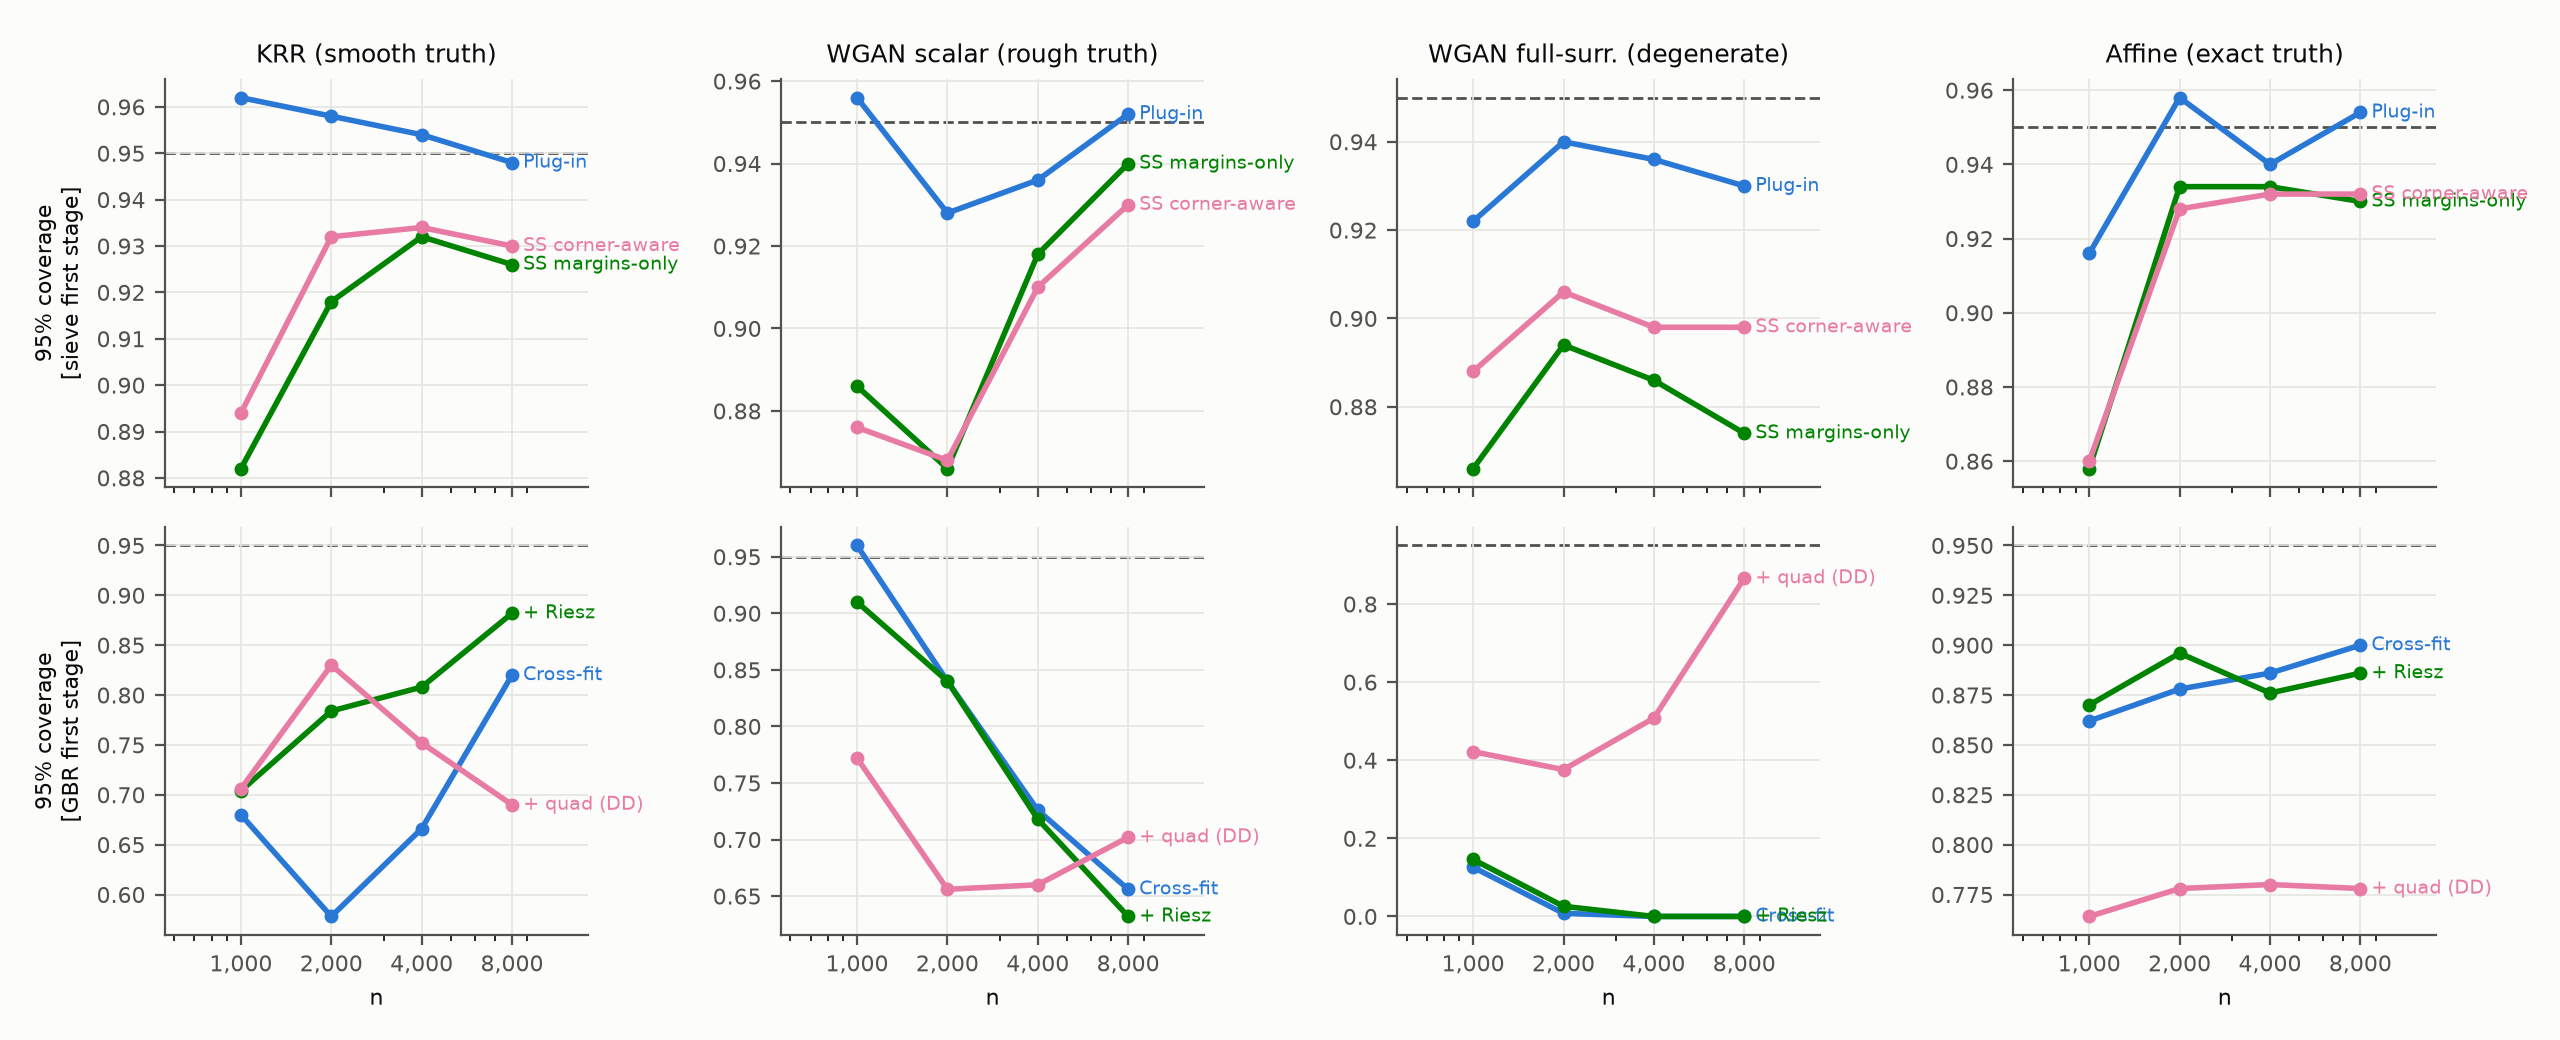
\includegraphics[width=\textwidth]{fig_debias_coverage.png}
\caption{Empirical 95\% coverage by sample size, DGP (columns), and
first-stage family (rows). Dashed line: nominal $0.95$.}
\label{fig:coverage}
\end{figure}

\begin{figure}[!htbp]
\centering
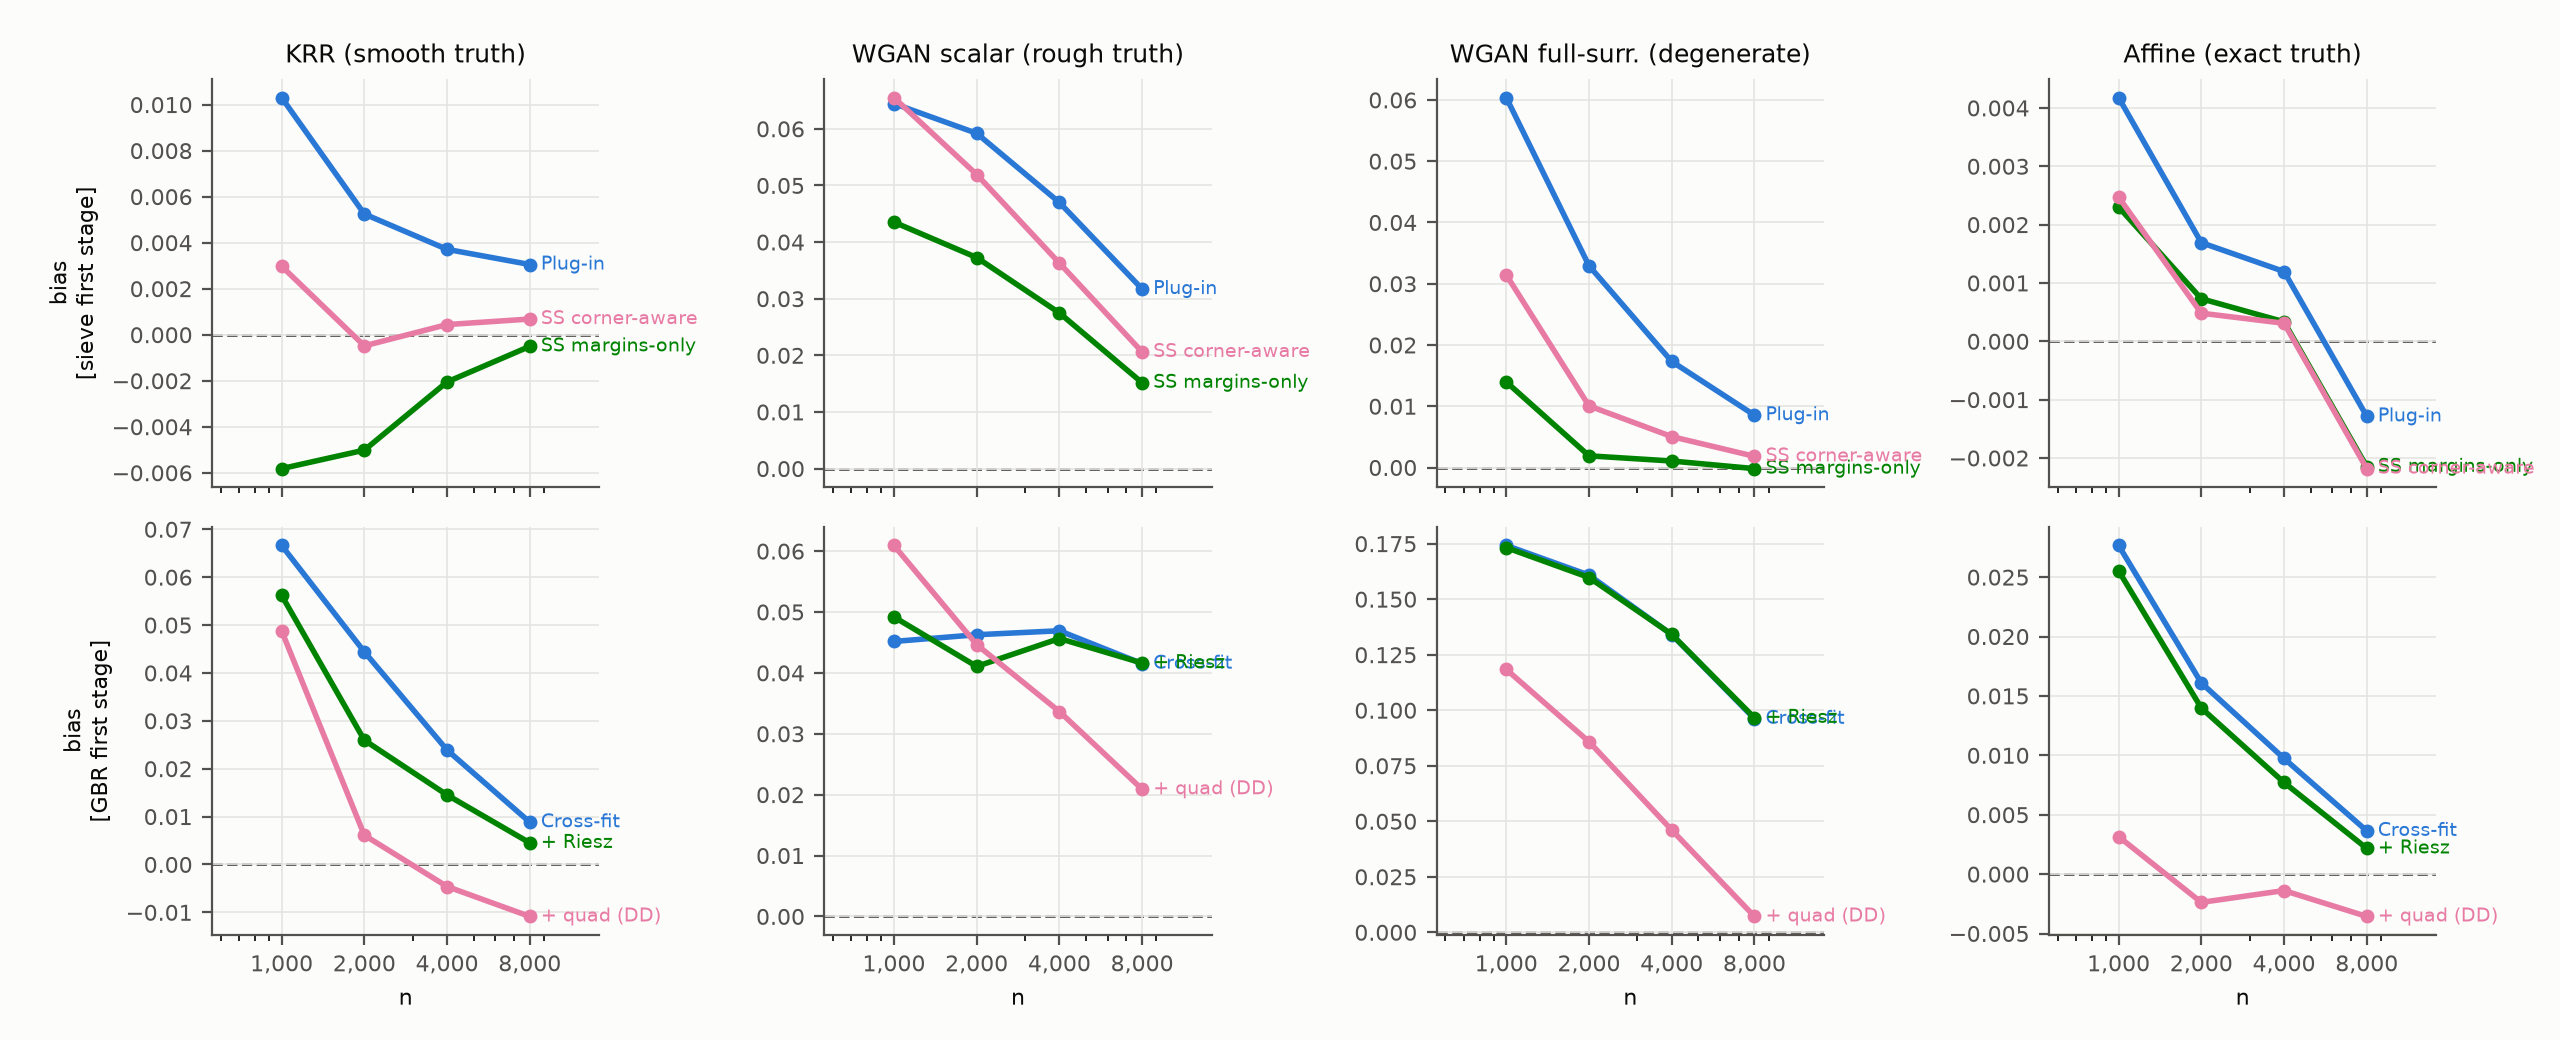
\includegraphics[width=\textwidth]{fig_debias_bias.png}
\caption{Monte Carlo bias by sample size, DGP, and estimator. Dashed
line: zero.}
\label{fig:bias}
\end{figure}

\begin{table}[!htbp]
\centering
\caption{Decomposition of the machine-learning undercoverage on the KRR
design ($n=4000$, $300$ replications). ``Plug-in bias'' is the uncorrected
cross-fit bias; ``bias'', ``SD'', ``SE/SD'', and ``coverage'' refer to the
Riesz-corrected estimator, studentized by \eqref{eq:two-band-var}. The
tensor-sieve plug-in is the reference. Varying folds, learner, and
representer basis one at a time isolates each mechanism of
Remark~\ref{rem:outofspan}. MC standard error of a coverage figure is about
$0.013$ at $300$ replications.}
\label{tab:dml-diag}
\begin{tabular}{lccccc}
\toprule
Configuration & Bias & Plug-in bias & SD & SE/SD & Coverage \\
\midrule
tensor-sieve plug-in & +0.0034 & +0.0034 & 0.0178 & 1.03 & 0.943\\
gbr K=2 riesz=sieve & +0.0216 & +0.0317 & 0.0186 & 0.96 & 0.760\\
gbr K=5 riesz=sieve & +0.0106 & +0.0160 & 0.0191 & 0.94 & 0.903\\
gbr K=10 riesz=sieve & +0.0079 & +0.0127 & 0.0196 & 0.92 & 0.913\\
rf K=5 riesz=sieve & +0.0119 & +0.0453 & 0.0195 & 1.01 & 0.907\\
krr K=5 riesz=sieve & +0.0038 & +0.0039 & 0.0184 & 0.90 & 0.917\\
gbr K=5 riesz=rf & +0.0078 & +0.0160 & 0.0203 & 0.96 & 0.937\\
krr K=5 riesz=rf & +0.0047 & +0.0039 & 0.0181 & 0.98 & 0.937\\
gbr(high-cap) K=5 riesz=sieve & +0.0439 & +0.0461 & 0.0131 & 1.00 & 0.077\\
gbr K=5 no correction & +0.0160 & +0.0160 & 0.0189 & 0.94 & 0.857\\
\bottomrule
\end{tabular}
\end{table}

\begin{figure}[!htbp]
\centering
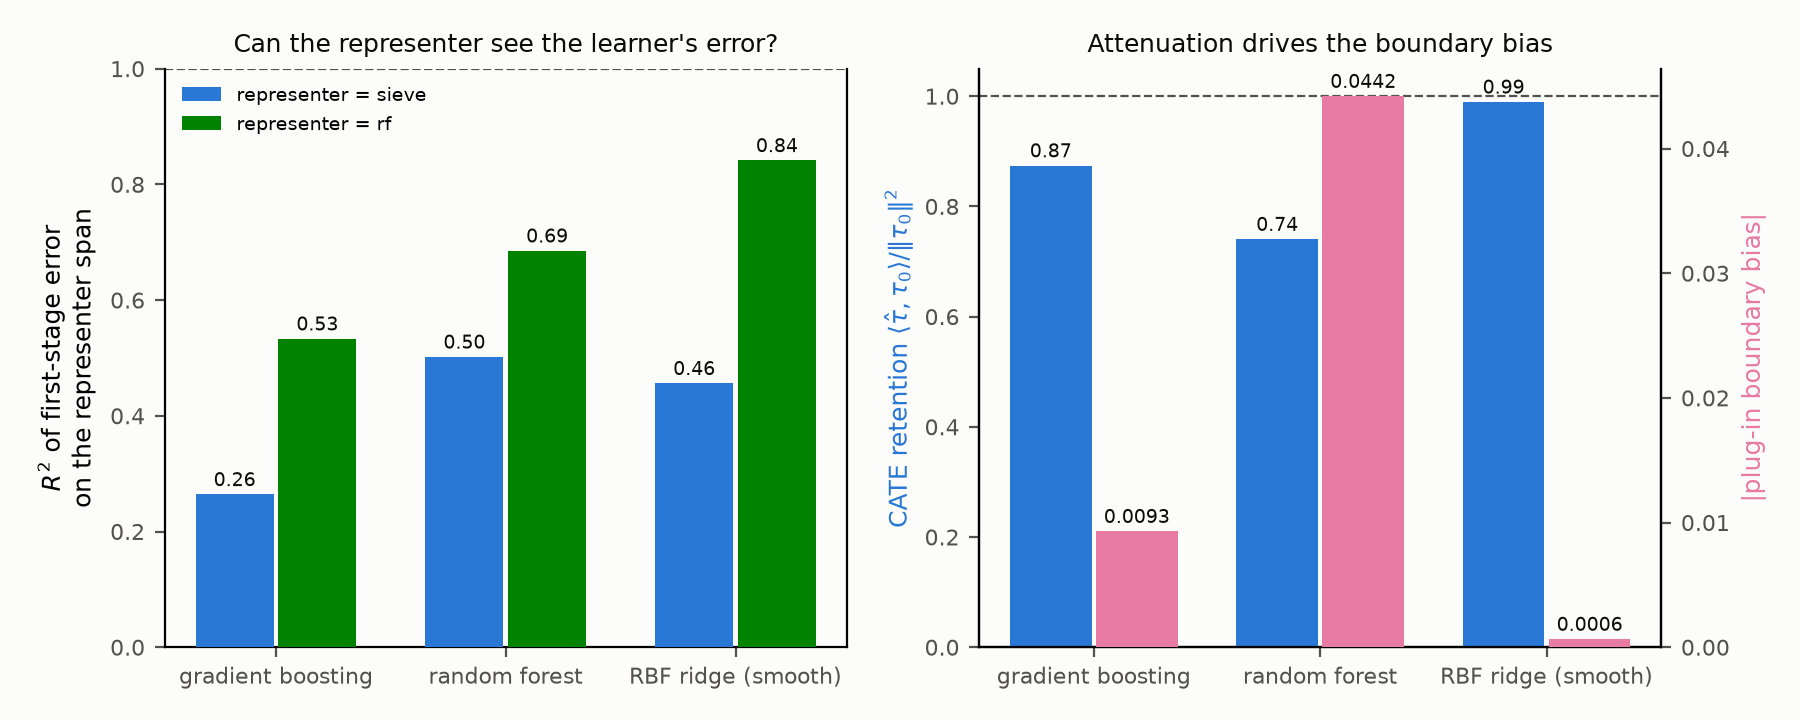
\includegraphics[width=\textwidth]{fig_dml_diagnosis.png}
\caption{Why boosting-based DML undercovers. \emph{Left}: the fraction
($R^{2}$) of the first-stage error that the sieve-Riesz representer can
span in global $L^{2}$, measured against the oracle arm means; a boosted-tree
error is largely invisible to a smooth representer, a random-feature ridge's
error is not. \emph{Right}: tree learners attenuate the CATE
(no-intercept projection coefficient of fitted on true, $\hat\tau'\tau/
\tau'\tau<1$), which displaces the decision boundary and biases the
plug-in; the smooth learner barely attenuates and is nearly unbiased. Both
panels average five simulated datasets and are indicative rather than
precise.}
\label{fig:dml-diag}
\end{figure}

\subsection{Corner anatomy}
\label{sec:anatomy}

Because the KRR oracle's contrast surfaces are known in closed form, the
corner set and its geometry are computable: the zero curves of $\tau_{S}$ and
$\tau_{Y}$ cross at ten points, with gradient norms
$\norm{\nabla\tau_{S}}\in[10.3,135.8]$, $\norm{\nabla\tau_{Y}}\in[13.9,56.4]$,
$\abs{\cos\omega}\leq0.90$ (transversality holds:
$\abs{\sin\omega}\geq0.45$), and within-unit residual correlation
$\rho_{SY}=0.524$. Table~\ref{tab:anatomy} traces the corner mechanism of
Section~\ref{sec:orders} across $300$ replications per sample size (sieve
first stage, fixed $K$).

\begin{table}[!htbp]
\centering
\caption{Corner anatomy on the KRR-calibrated oracle (300 reps, fixed
sieve dimension). ``Total'' is the implied plug-in corner bias
$\sum_{x^{*}}\E[\Delta_{g}\Delta_{h}]\,w/
(\Ng\Nh\abs{\sin\omega})$ in $\theta$ units;
``SS estimate'' is the mean corner cross correction
$\widehat{\text{corner}}$ of \eqref{eq:polarization}, which by split-sample
independence targets the \emph{stochastic} ($K/n$) part of the
diagonal; ``remainder'' is their difference, the bias-product
($K^{-2s/d}$) part. Sign convention: the anatomy script measures
$\E[\Delta\hat\tau_{S}\,\Delta\hat\tau_{Y}]$ (positive here, as
$\rho_{SY}>0$); the table reports the corner term in $\theta$ units, where
the harm-share convention $h_{0}=-\tau_{Y}$ flips its sign.
$\overline{\text{corr}}$ averages
$\mathrm{Corr}(\Delta_{g}(x^{*}),\Delta_{h}(x^{*}))$ over the ten corners.
The column implements the corner \emph{cross} term
$\mathcal B_{\Corner}^{\times}$ of Proposition~\ref{prop:margins} --- the
first term of the bracket in \eqref{eq:corner-coef} --- which by
\eqref{eq:polar-limit} is exactly the quantity that margins-only debiasing
leaves behind and that $\widehat{\mathrm{corner}}$ targets, so the comparison
across columns is like-for-like. It is \emph{not} the corner's full
contribution to the plug-in bias, which also contains the two
$\cos\omega$-weighted diagonals of \eqref{eq:corner-coef} (non-negligible
here, since $\abs{\cos\omega}$ reaches $0.90$) but which margins-only
debiasing already removes. The column also uses an unnormalized covariate
density (Section~\ref{sec:limits}, item~(L2)).}
\label{tab:anatomy}
\begin{tabular}{lccccc}
\toprule
$n$ & Total corner bias & SS estimate & Remainder &
$\overline{\text{corr}}(\Delta_{g},\Delta_{h})$ & $\rho_{SY}$\\
\midrule
2000 & $-0.0080$ & $-0.0044$ & $-0.0036$ & $0.50$ & $0.524$\\
4000 & $-0.0048$ & $-0.0022$ & $-0.0025$ & $0.46$ & $0.524$\\
8000 & $-0.0038$ & $-0.0012$ & $-0.0026$ & $0.45$ & $0.524$\\
\bottomrule
\end{tabular}
\end{table}

Three predictions of Section~\ref{sec:orders} are consistent with the table.
\emph{(i)} The pointwise correlation of the two surface errors at the corner
tracks the within-unit residual correlation ($0.45$--$0.50$ against
$\rho_{SY}=0.524$), which is the mechanism behind the $V_{gh}$ term in
\eqref{eq:corner-coef}. \emph{(ii)} The stochastic part of the corner
diagonal halves as $n$ doubles at fixed $K$
($-0.0044\to-0.0022\to-0.0012$) --- the $K/n$ scaling --- and is tracked by
the SS corner correction, which by construction cancels bias parts across the
two independent halves. \emph{(iii)} The remainder is roughly constant in $n$
at fixed $K$ ($-0.0036$ at $n=2000$, then $\approx-0.0025$), as befits the
$K^{-2s/d}$ bias product, which is controlled by undersmoothing $K$ rather
than by debiasing --- and which, per Proposition~\ref{prop:margins}, the SS
statistic is not supposed to capture. The measured corner bias
($0.4$--$0.8$ percentage points of a $\theta_{0}=0.161$ target)
is material relative to the plug-in standard error, and its sign matches the
Monte Carlo finding that the corner-aware and margins-only SS estimates
differ by $+0.004$ to $+0.005$ at $n=2000$. This validates the cross-corner
component of \eqref{eq:corner-coef} --- the component that
Proposition~\ref{prop:margins} says is at stake in the margins-only
comparison. The two $\cos\omega$ components of \eqref{eq:corner-coef} are not
tested here, because both debiasing variants remove them; testing them would
require comparing the \emph{plug-in} against a corner-corrected plug-in.

\subsection{A fixed-$K$ diagnostic for the cross-half off-diagonal}
\label{sec:offdiag}

Table~\ref{tab:mc-main} contains, without any further computation, a
diagnostic for the $n$-dependence of the off-diagonal bound derived in
Appendix~\ref{app:proofs}, \S B.2. Because the design holds $K$ fixed, it
cannot test the exponent on $K$ that enters Theorem~\ref{thm:ss}(ii)'s
window \eqref{eq:ss-window}.

The SS estimator's error differs from the plug-in's by removing the
stochastic diagonal and adding the mean-zero cross-half term
$\tfrac12D^{2}\Th[u^{A},u^{B}]$. By \S B.2 that term has variance
$\asymp n^{-2}K_{n}^{(d+3)/d}$, against a score variance
$\sigma_{n}^{2}/n\asymp K_{n}^{1/d}/n$. Since the two estimators use the same
observations and the same standard error, this predicts
\begin{equation}
\frac{\mathrm{SD}(\hat\Th_{SS})}{\mathrm{SD}(\hat\Th)}
=\sqrt{1+c\,\frac{K_{n}^{(d+2)/d}}{n}}\,(1+o(1)),
\qquad c\ \text{constant in }n,
\label{eq:sdratio}
\end{equation}
which at the design's fixed $K=25$, $d=2$ is $\sqrt{1+625c/n}$. Writing
$R_{n}$ for the observed ratio $\mathrm{SD}_{SS}/\mathrm{SD}_{\text{plug-in}}$,
the implied $c=n(R_{n}^{2}-1)/K^{2}$ should be flat in $n$:
\begin{center}
{\small
\setlength{\tabcolsep}{5pt}
\begin{tabular}{lccccc}
\toprule
Design & $n=1000$ & $2000$ & $4000$ & $8000$ & spread \\
\midrule
Affine (exact truth; assumptions hold) & $0.89$ & $1.10$ & $1.01$ & $1.07$
 & $1.2\times$\\
KRR (smooth) & $0.83$ & $0.90$ & $1.38$ & $0.19$ & $7.2\times$\\
WGAN scalar ($s\approx1$; violates) & $1.36$ & $2.83$ & $3.80$ & $5.05$
 & $3.7\times$\\
WGAN degenerate (empty margins; violates) & $1.94$ & $3.33$ & $10.39$
 & $15.69$ & $8.1\times$\\
\bottomrule
\end{tabular}}
\end{center}
On the affine design --- the only one with an exactly closed-form truth and
all maintained assumptions satisfied --- $c$ is flat within a factor $1.2$
and centered on $1$, across a factor of eight in $n$, with no fitted
parameter beyond the $\asymp$ constant itself. On KRR the first three cells
agree; the $n=8000$ cell is uninformative, since there
$(\mathrm{SD}_{SS}/\mathrm{SD}_{\text{plug-in}})^{2}-1=0.016$ is of the order
of the Monte Carlo error of a ratio of two standard deviations estimated
from 500 replications (we have not computed that error, which is smaller
than an independent-samples calculation would give, since the two use
\emph{common} replications). The two designs that violate the maintained
assumptions show $c$ increasing monotonically by factors of $3.7$ and $8.1$,
flatly inconsistent with \eqref{eq:sdratio}. The test therefore
discriminates across these designs rather than merely fitting a constant,
but it remains a fixed-$K$ check of the $1/n$ component only.

Two corollaries. First, this numerically accounts for the SS standard
error's calibration. Because the implementation computes one standard error
from the full-sample fit and applies it to both estimators, SE/SD for SS must
equal (SE/SD for the plug-in) divided by the SD ratio, as an identity; and
indeed the reported values agree to within $0.003$--$0.008$ on all four
designs and all four sample sizes. The SS SE/SD deficit of
$0.78$--$0.96$ is thus consistent with the variance of the quadratic
correction, which the first-order standard error omits by construction ---
not a failure of the two-band variance formula, and not the corner.

Second, the finite-sample formula mirrors a condition in
Theorem~\ref{thm:ss}(ii). The inflation factor $K_{n}^{(d+2)/d}/n$ vanishes
precisely when $a<d/(d+2)$, which is the \emph{upper edge of the window}
\eqref{eq:ss-window}. This algebra explains why that edge appears, but the
fixed-$K$ experiment does not test it. At the design's fixed $K=25$ the factor is
$0.63,0.31,0.16,0.08$ --- large at $n=1000$, still $8\%$ at $n=8000$ --- and
a growing-$K_{n}$ implementation inside \eqref{eq:ss-window} is exactly what
would drive it away. A standard error for $\hat\Th_{SS}$ that included the
correction's own variance would fix the calibration at fixed $K$; we do not
currently have one.

\subsection{Results}\label{sec:results}

Table~\ref{tab:mc-main} and Figures~\ref{fig:coverage}--\ref{fig:bias}
report all cells; Section~\ref{sec:limits} states which conclusions they can
and cannot support.

\emph{(1) Smooth truth (KRR): the plug-in is already good; corner-aware SS
removes what bias there is.} The plug-in covers at $0.948$--$0.962$ at all
$n$ with a small decaying bias ($+0.010\to+0.003$) and a well-calibrated
standard error (SE/SD $0.94$--$1.11$, tightening toward one with $n$). SS
debiasing removes the bias essentially completely ($+0.003\to+0.0007$; a
$3.5$-fold bias reduction at $n=1000$ and a tenfold reduction at $n=2000$),
at a variance cost that is $23\%$ of the standard deviation at $n=1000$ and
falls to $10\%$ at $n=4000$ and about $1\%$ at $n=8000$ ---
Section~\ref{sec:offdiag} shows this is the cross-half term
$\tfrac12D^{2}\Th[u^{A},u^{B}]$, decaying as
$1/n$ predicts at the fixed $K$ used here, and that it accounts for the whole
of the SS coverage shortfall. The
\emph{margins-only} correction overshoots to negative bias
($-0.006$ to $-0.0005$) at every $n$: it removes the (positive) margin
diagonals --- and, per \eqref{eq:polar-limit}, the two $\cos\omega$ corner
diagonals as well --- but not the (negative) corner \emph{cross} term. The gap
between the corner-aware and margins-only estimates equals the estimated
corner correction ($\hat\Th_{SS}=\hat\Th_{SS}^{\text{mar}}
-\widehat{\text{corner}}$) and matches the anatomy of
Table~\ref{tab:anatomy} to the fourth decimal ($+0.0045$ at $n=2000$
against minus the anatomy's SS corner estimate of $-0.0044$).
The raw corner cross form $q_{\text{full}}-q_{g}-q_{h}$ (eight times the
corner correction) halves as $n$ doubles
($-0.070\to-0.036\to-0.020\to-0.0095$) at fixed $K$, consistent with the
$1/n$ component of \eqref{eq:corner-coef}; it does not test the exponent on
$K$. Coverage of the SS intervals is $0.894$--$0.934$
on this design: an improvement in centering bought at a $2$--$5$ point
coverage cost relative to the plug-in, which we do not describe as honest
coverage.

\emph{(2) Rough truth (scalar WGAN, $s\approx1$): debiasing accelerates the
bias decay.} This design violates the smoothness hypothesis of every theorem
above ($s\approx1<(d+1)/2=1.5$), so it is a robustness probe. The plug-in
bias is large and decays at only $\approx n^{-0.34}$ ($+0.064\to+0.032$),
and its near-nominal coverage rests on a conservative SE (SE/SD
$1.1$--$1.3$). SS debiasing accelerates the empirical decay to
$\approx n^{-0.55}$ ($+0.066\to+0.021$) with SE/SD $0.83$--$0.98$ and
coverage $0.87\to0.93$. Because $K$ is fixed across $n$ here, these
exponents describe the finite-sample behavior of the estimators at $K=25$;
they are not estimates of the asymptotic rate, which would require
$K_{n}$ to grow (Section~\ref{sec:limits}, item~(L4)). On this rough truth
the margins-only variant is slightly better centered than the corner-aware
one --- with $s\approx1$ the corner correction is itself noisily estimated
--- a useful caution: corner-awareness is a bias-\emph{decomposition}
necessity, but its sampled version adds noise when the surfaces are rough.

\emph{(3) Machine-learning first stages: the projected Riesz correction
works where the learner is adequate; the quadratic correction is not a free
lunch.} On the smooth truth the GBR bias falls monotonically along the
ladder cross-fit $\to$ $+$Riesz $\to$ $+$quadratic at every $n$ (at
$n=4000$: $+0.024\to+0.015\to-0.005$), consistent with the two corrections
targeting distinct error terms. But the composition has two finite-sample
costs: the SS-on-GBR quadratic correction inflates the dispersion (by a
factor of two at $n=1000$, $1.4$ thereafter), and the first-order SE does
not account for it (SE/SD $\approx0.6$), so DD
intervals undercover ($0.69$--$0.83$); and at $n=8000$ on KRR the
quadratic correction overshoots ($-0.011$). \emph{This ladder must now be
read with item~(L7) of Section~\ref{sec:limits} in hand}: the DD column
implements the superseded construction \eqref{eq:dd-v2}, whose second-order
bias $-\tfrac12\{D^{2}\Th[e_{A},e_{A}]+D^{2}\Th[e_{B},e_{B}]\}$ predicts
exactly this over-correction and this dispersion inflation, on smooth and
rough designs alike. v2 attributed the overshoot to
Remark~\ref{rem:tree-jack} --- \eqref{eq:jackknife} being a fourth-order
finite difference of a step function for tree first stages --- which is a
real effect but cannot explain the same pattern on the affine design. On the
rough truth GBR is bias-limited ($+0.045$ nearly flat in $n$; coverage falls
to $0.64$): no first-order correction can rescue a nuisance that misses the
kinks. The degenerate arm is the extreme case: GBR manufactures a spurious
harm share of $+0.17$ (coverage $0$), and there the quadratic correction
\emph{does} rescue it ($+0.007$, coverage $0.87$ at $n=8000$).

\emph{(4) The two-band SE is well calibrated for the sieve family.} The
variance estimator \eqref{eq:two-band-var} includes the empirical-measure
term $\hat\varsigma^{2}/n=\hat\theta(1-\hat\theta)/n$ --- the sampling error
of the average given the surfaces, the analogue of the
$\mathrm{Var}([h_{0}]_{+})$ term the single-threshold unknown-density welfare
theorem adds --- which is $6$--$12\%$ of the SE at these sample sizes and, if
omitted, produces a spurious SE/SD of $0.87$--$0.95$. With it included,
SE/SD is $0.90$--$1.11$ for plug-in and SS on the KRR and affine designs, and
the studentized intervals reach $0.93$--$0.95$ by $n=8000$; on the
degenerate arm ($\theta_{0}=0$, empty margins) the sieve family degrades
gracefully.

\emph{(5) Machine-learning first stages: why the sieve-DML interval
undercovers, and when it does not.} The cross-fitted GBR estimators cover
only $0.58$--$0.88$ on the smooth design, in sharp contrast to the sieve
plug-in on the \emph{same samples} --- so the shortfall is a property of the
first stage, not the DGP or the variance formula. The diagnosis is
Remark~\ref{rem:outofspan}. Measured against the oracle arm means, the
$R^{2}$ of the boosted first-stage error on the tensor B-spline representer
span is $0.21$--$0.34$ across the four arm regressions (mean $0.26$); the
projected correction removes $31\%$ of the plug-in's boundary bias. The
direct variance test reported in Remark~\ref{rem:outofspan} shows that the
remaining $69\%$ is \emph{bias}, not an independent added variance: the
leading explanation is that the correction cannot see the part of the
learner's error that lives on the margins, so it leaves the boundary
displaced. Three levers move coverage:
\emph{(i) folds} --- $K=2\to5\to10$ lifts GBR coverage $0.76\to0.90\to0.91$
by shrinking the own-observation bias trained on $(K-1)/K$ of the sample;
\emph{(ii) representer basis} --- matching a $400$-feature random-feature
representer to the boosted learner raises the projected $R^{2}$ from $0.26$
to $0.53$ and coverage from $0.90$ to $0.94$; \emph{(iii) learner
smoothness} --- a random-feature (RBF) ridge, whose error the representer
\emph{can} span ($R^{2}=0.84$), attenuates the CATE by only about $1\%$
(against boosting's $13\%$) and has a plug-in bias of $+0.0006$ (against
$+0.016$), so there is almost nothing left to correct and, with a matched
representer, it too reaches $0.94$. Higher-capacity boosting is
counterproductive --- it sharpens the axis-aligned staircase, driving
coverage toward zero. The pattern reproduces the parent draft's own
single-threshold Table~7. The residual $0.01$--$0.02$ shortfall of even the
best machine-learning cell below the sieve plug-in's coverage is within
two Monte Carlo standard errors and should not be over-interpreted.

\subsection{What the current Monte Carlo does and does not
establish}\label{sec:limits}

The tables above are reproduced from v1 without change. Auditing the code
against the theory turned up seven implementation gaps. None of them affects
Theorem~\ref{thm:D2} or the order accounting of Section~\ref{sec:orders},
which are analytic; all of them bear on how much weight the simulation
evidence can carry, and all are scheduled for repair before the next
revision. We list them explicitly rather than leave them implicit.

\begin{description}[leftmargin=2.2em,style=nextline]
\item[(L1) The KRR ``oracle truth'' is displaced by uncentered residual
resampling.] The sampler draws outcome noise by resampling the fitted
per-arm KRR residual pools, which are not centered (ridge shrinkage leaves
arm-specific residual means). The generated conditional means therefore
differ from the nominal KRR surfaces by a constant per arm, shifting the
generated CATEs by $\Delta\tau_{S}=+0.126$ and $\Delta\tau_{Y}=+0.182$
(the latter includes the short$\to$long coupling). The reported truth
$\theta_{0}$ moves from $0.16115$ to $0.15998$ --- immaterial for the bias
columns --- but the ten corner locations, gradients, angles, and first-stage
errors used in Table~\ref{tab:anatomy} are all computed against the
\emph{wrong} surfaces. Fix: center each arm's residual pool before
resampling, or define the oracle truth to include the shifts.
\item[(L2) The corner density is unnormalized.] Covariates are drawn from
the KDE conditional on $X\in[-3,3]^{2}$ by rejection sampling, but the
density accessor returns the untruncated KDE. The KDE mass of the box is
$0.807$, so the corner integrals in Table~\ref{tab:anatomy} should be scaled
by $1/0.807\approx1.24$ before any comparison with
\eqref{eq:corner-coef}. Together with the omission of the $\cos\omega$ terms
noted in the table caption, the ``Total'' column is an incomplete
implementation of the theory it is meant to check.
\item[(L3) The KRR design violates Assumption~\ref{ass:geometry}(d).] The
KDE density is positive at the truncation boundary, and a direct scan of the
four box edges finds twelve sign crossings of the two contrast surfaces
($\tau_{S}$: three on $x_{1}=-3$, two on $x_{1}=+3$, three on $x_{2}=-3$;
$\tau_{Y}$: two on $x_{1}=-3$, two on $x_{2}=+3$). The margins therefore
terminate at the support edge, and by Remark~\ref{rem:edge} the correct
second derivative for this DGP carries additional support-edge
$\Haus^{d-2}$ terms that \eqref{eq:D2} omits. Fix: taper $w$ near
$\partial\mathcal X$, or shrink the box so that all margins close inside it.
\item[(L4) The main Monte Carlo holds $K$ fixed.] Every sample size uses two
knot segments per coordinate, i.e.\ $K=25$ basis functions per arm at every
$n$. The design therefore does not implement
$K_{n}\asymp n^{d/(2s+1)}$, and the estimated log-rate slopes reported in
Section~\ref{sec:results}(2) are not estimates of the asymptotic rate. At
fixed $K$ the design can reveal the predicted $1/n$ decline of the corner
diagonal, but it cannot test the exponent on $K$ in the $K/n$ bound
(Table~\ref{tab:anatomy}).
\item[(L5) The variance bandwidth does not satisfy
Proposition~\ref{prop:var}.] The implementation sets
$\varepsilon=\delta\cdot\widehat{\mathrm{sd}}(\hat\tau)$ with $\delta$ fixed
and then widens $\varepsilon$ by factors of $1.5$ until at least five
observations enter the band. Since $\widehat{\mathrm{sd}}(\hat\tau)$
converges to a positive constant, $\varepsilon_{n}\not\to0$, contradicting
Proposition~\ref{prop:var} and Assumption~\ref{ass:dml}(b). On the
degenerate arm the widening manufactures a nonempty derivative band where
the population margin is empty. Fix: $\varepsilon_{n}=\delta_{n}\cdot
\widehat{\mathrm{sd}}(\hat\tau)$ with $\delta_{n}\to0$ at a rate satisfying
$n\varepsilon_{n}/K_{n}\to\infty$.
\item[(L6) The coded Riesz correction is not fold-specific.] Both the
cross-fitted DML estimator and the DD estimator build a single full-sample
Gram matrix and band representer from pooled out-of-fold predictions, whereas
\eqref{eq:dml} and Theorem~\ref{thm:dml} require an off-fold representer for
each fold. In the implementation, observation $i$'s outcome can influence the
global band through the model trained on $i$'s own fold, which breaks the
conditional mean-zero step used in Remark~\ref{rem:outofspan}. Fix: build
$\hat v^{*}_{-\kappa}$ inside the fold loop.
\item[(L7) The DD rows implement the superseded construction
\eqref{eq:dd-v2}.] Every ``$+$ quad.\ (DD)'' cell of
Table~\ref{tab:mc-main} evaluates $\hat\Th^{\,\mathrm{v2}}_{DD}$, which by
Remark~\ref{rem:ddbug} carries a second-order bias
$-\tfrac12\{D^{2}\Th[e_{A},e_{A}]+D^{2}\Th[e_{B},e_{B}]\}$ that the
corrected estimator of Definition~\ref{def:dd} does not. These cells
therefore say nothing about Theorem~\ref{thm:dd}. They are, however,
\emph{consistent} with the diagnosis: since the uncorrected plug-in bias is
positive on every design, the corresponding $D^{2}\Th[e,e]$ diagonal has the
same sign, and the extra minus coefficient reverses it, predicting an
over-correction into negative territory, which is what
the smooth designs show ($-0.0046$ and $-0.0109$ at $n=4000,8000$ on KRR;
$-0.0024$ to $-0.0036$ on Affine) together with the dispersion inflation
(SE/SD $\approx0.6$ throughout). v2 attributed this over-correction to the
non-smoothness of tree first stages (Remark~\ref{rem:tree-jack}); the
structural defect is the better explanation, because it is present for the
smooth (KRR, affine) designs as well, where the tree explanation does not
apply. Fix: implement Definition~\ref{def:dd} with three folds.
\end{description}

Taken together: Theorem~\ref{thm:D2} is derived analytically and checked
numerically (Appendix~\ref{app:numeric}); the $1/n$ component and the sign and
magnitude of the corner correction are consistent with
Tables~\ref{tab:anatomy} and~\ref{tab:mc-main} at $d=2$ and fixed $K$, but
the $K$ exponent is not tested. These readings are subject to (L1)--(L3).
The cross-half off-diagonal order
$n^{-1}K_{n}^{(d+3)/(2d)}$ of Appendix~\ref{app:proofs}, \S B.2 --- which
sets the upper edge of the SS window \eqref{eq:ss-window} --- has its
fixed-$K$ $1/n$ implication supported by Section~\ref{sec:offdiag} on the
designs that satisfy the assumptions; its $K_n$ exponent remains untested.
The asymptotic
rate claims of
Theorems~\ref{thm:plugin}, \ref{thm:ss}, \ref{thm:dml} and~\ref{thm:dd} are
\emph{not} tested by the present design, because $K$ does not grow with $n$;
the DD cells test a construction we have since shown to be invalid, (L7);
and the mechanism behind the machine-learning undercoverage is identified as
residual boundary bias rather than unmodelled variance, by the direct
variance test in Remark~\ref{rem:outofspan}.

\emph{Practical guidance.} We state it narrowly, because
Section~\ref{sec:limits} limits what the experiments support and
Section~\ref{sec:dml} limits what the theory establishes.

For sieve first stages, the corner-aware SS estimator \eqref{eq:jackknife}
with the two-band SE is the recommendation: it is tuning-free and removes the
second-order stochastic diagonal including the corner. In our designs its
centering is clearly better than the plug-in's and its coverage is $2$--$5$
points worse ($0.894$--$0.934$ on KRR), so it buys bias reduction at a
coverage cost; we would not call its intervals honest. Undersmoothing
relative to $K_{n}\asymp n^{d/(2s+1)}$ is required for the interval to be
centered at all --- window \eqref{eq:ss-window} --- and the fixed-$K$ Monte
Carlo does not exercise this.

For a machine-learning first stage --- needed when $d$ is too large for a
tensor sieve --- prefer a \emph{smooth} learner and \emph{match the
representer basis to the learner's own feature map}, so the projected
correction is near-exact; avoid tree ensembles, whose piecewise-constant
error is largest precisely on the margins the representer must span; and use
at least five folds for the nuisance cross-fit. (This concerns the number of
\emph{nuisance} folds and does not conflict with the two-half construction of
$\hat\Th_{SS}$: there, the two halves furnish the independent replicates that
the polarization identity \eqref{eq:ss-identity} requires, and $K=2$ is part
of the definition of the quadratic correction, not a cross-fitting choice.
The corrected DD estimator of Definition~\ref{def:dd} needs a third fold on
top of that.) When a tree first stage is unavoidable, pair it with a
full-refit bootstrap rather than the analytic SE.

We do \emph{not} currently recommend the doubly debiased estimator in
applied work. The construction evaluated in Table~\ref{tab:mc-main} is
invalid (Remark~\ref{rem:ddbug}); the corrected construction of
Definition~\ref{def:dd} has not been implemented or simulated; and even for
it, Theorem~\ref{thm:dd} is conditional on remainder bounds we have not
established and excludes tree first stages outright.

The comparison of the corner-aware and margins-only corrections is a useful
specification diagnostic in its own right: their gap estimates the corner
cross term, whose magnitude flags whether the two-threshold structure is
quantitatively binding.

\appendix

\section{Derivation of the Second Derivative (Theorem~\ref{thm:D2})}
\label{app:D2}

Write $T_{g}(t):=\int_{\{g_{t}=0\}\cap\{h_{t}\geq0\}}
\varpi_{t}\dd\Haus^{d-1}$ with weight
$\varpi_{t}:=u\,w/\norm{\nabla g_{t}}$ (we reserve $\omega(x)$ for the
transversality angle throughout), the first term of \eqref{eq:D1}
along $\gamma_{t}$; the second term is symmetric. Let
${\bf X}(\cdot,t)$ be the normal diffeomorphism carrying
$\mathcal M:=\{g_{0}=0\}$ to $\{g_{t}=0\}$ with velocity
$\dot{\bf X}=-(u/\Ng)\,n_{g}$, and pull the integral back
to $\mathcal M$:
\[
T_{g}(t)=\int_{\mathcal M}
\1\{h_{t}({\bf X}(x,t))\geq0\}\;
\varpi_{t}({\bf X}(x,t))\,J_{\bf X}(x,t)\dd\Haus^{d-1}(x).
\]
Differentiating at $t=0$ yields four contributions.
\emph{(1) Integrand:} $\partial_{t}\varpi_{t}
=-u\,w\,(n_{g}\!\cdot\!\nabla u)/\Ng^{2}$.
\emph{(2) Transport of $\varpi$ and area:} by the surface-transport formula
\citep[Ch.~9]{dz2001},
$\partial_{t}\{\varpi({\bf X})J_{\bf X}\}
=-\big[(u/\Ng)\,n_{g}\!\cdot\!\nabla\varpi
+\varpi\,(u/\Ng)H_{g}\big]$, the moving-level-set terms of
\citet[Lem.~PathD--Level]{cg2026} with weight $\varpi$.
\emph{(3) Direct motion of the cut:} the indicator
$\1\{h_{t}\geq0\}$ evaluated on the (fixed, $t=0$) manifold defines the
region $\{h_{0}+tv\geq0\}\cap\mathcal M$; by the within-manifold Leibniz
rule its derivative is an integral over the relative boundary
$\Corner$ with normal velocity $v/\norm{\nabla_{\!\mathcal M}h_{0}}$, where
$\norm{\nabla_{\!\mathcal M}h_{0}}=\norm{P_{T}\nabla h_{0}}
=\Nh\abs{\sin\omega}$, giving
$+\int_{\Corner}\varpi_{0}\,v/(\Nh\abs{\sin\omega})
\dd\Haus^{d-2}$ --- the cross term.
\emph{(4) Induced motion of the cut:} the composition
$h_{0}({\bf X}(x,t))=h_{0}(x)-t\,(u/\Ng)\,
n_{g}\!\cdot\!\nabla h_{0}+o(t)
=h_{0}(x)-t\,u\,\Nh\cos\omega/\Ng+o(t)$
perturbs the cut function by an effective
$v_{\text{eff}}=-u\Nh\cos\omega/\Ng$;
the same within-manifold Leibniz rule then contributes
$-\int_{\Corner}\varpi_{0}\,u\cos\omega/
(\Ng\abs{\sin\omega})\dd\Haus^{d-2}$ --- the diagonal
corner term of \eqref{eq:Qg}. Collecting (1)--(4), and adding the symmetric
derivative of the $\Mh$-term (which contributes the mirror-image margin
form, the second copy of the cross term, and the $v^{2}$ diagonal corner
term), gives \eqref{eq:D2}--\eqref{eq:Qg}. Transversality bounds every
corner integrand; twice-differentiability of $g_{0},h_{0}$ and
Assumption~\ref{ass:model}(d) bound the curvature and gradient terms.
$\hfill\square$

\section{Orders of the Remainder Terms}\label{app:proofs}

The margin components of all remainder bounds are adaptations of the
single-threshold arguments --- \citet[Thms.~5, 8 and the SS/LOO
constructions]{cg2026} for the quadratic terms, and the extended
single-threshold draft (sieve-DML theorem and its Assumption~5) for the
cross-fitted first-order correction --- applied margin by margin with the
truncation indicators carried as bounded weights. This appendix records the
two order calculations that are specific to the two-threshold geometry and
that v1 got wrong.

\subsection*{B.1 Why the margin diagonal is $K_{n}^{1+1/d}/n$}

Substituting the stochastic part \eqref{eq:decomp} into $Q_{g}$ and
writing
$\zeta_{g,i}(x):=\sum_{w}q_ws_{w,i}(x)\epsilon_{S,i}$, then separating
$i=j$ from $i\neq j$,
\[
Q_{g}[u_{g},u_{g}]
=\underbrace{\frac1{n^{2}}\sum_{i}Q_{g}[\zeta_{g,i},\zeta_{g,i}]}
_{T_{\mathrm{diag}}}
+\underbrace{\frac1{n^{2}}\sum_{i\neq j}
Q_{g}[\zeta_{g,i},\zeta_{g,j}]}_{T_{\mathrm{off}}} .
\]
The leading integrand of $Q_{g}$ carries one gradient, so
$\E\,Q_{g}[\zeta_{g,i},\zeta_{g,i}]$ involves an arm-wise sum of terms
\[
\psi(x)'R_w^{-1}\Omega_{SS}^{w}R_w^{-1}\nabla\psi(x),
\]
whose modulus is
$\lesssim K_{n}^{1+1/d}$ by \eqref{eq:sieve-scaling}, whence
$\E\,T_{\mathrm{diag}}=O(n^{-2}\cdot n\cdot K_{n}^{1+1/d})
=O(K_{n}^{1+1/d}/n)$. This is the \emph{bound} stated by \citet{cg2026} for
the single-threshold value functional, and it is the bound that
Table~\ref{tab:orders} records. The one-sided form is deliberate: the
quantity is signed, and Remark~\ref{rem:cancel} shows that its surface
integral can be an order smaller. The curvature part of $Q_{g}$, which
carries no gradient, contributes $O(K_{n}/n)$.

The corner forms in \eqref{eq:D2}--\eqref{eq:Qg} carry \emph{no} gradient of
$u$ or $v$. Their diagonals therefore involve
$\mathcal V_{gg,n}(x),\mathcal V_{hh,n}(x)\asymp K_n$ and the signed
$\mathcal V_{gh,n}(x)=O(K_n)$ from \eqref{eq:sandwich}, and are
$O(K_{n}/n)$: bounded by $K_{n}^{-1/d}$ times the margin bound. v1's assertion
that the corner diagonal is ``of the same order $K_{n}/n$ as the margin
diagonals'' conflated a bound with an exact order.

Two asymmetries between the two statements should be recorded.
\emph{(i)} The two pointwise corner variance building blocks are
$\asymp K_n/n$, while the cross-covariance block is only $O(K_n/n)$ and can
vanish. Every \emph{integrated signed} corner coefficient remains only an
upper bound unless Assumption~\ref{ass:cornernc} is imposed.
\emph{(ii)} The margin order is a bound only. In the homoskedastic,
constant-propensity special case,
$\E[\zeta_{g,i}\,\partial_{n}\zeta_{g,i}]$ is proportional to
$\tfrac12\partial_{n}\mathcal V$ for the corresponding effective leverage
function, and $\mathcal V$ oscillates at the mesh scale with
amplitude $\asymp K_{n}$, so while $\norm{\nabla\mathcal V}_{\infty}\asymp
K_{n}^{1+1/d}$ pointwise, the surface integral in \eqref{eq:gradV} can
cancel. Expanding $\mathcal V=\bar{\mathcal V}+\tilde{\mathcal V}$ with
$\tilde{\mathcal V}$ mesh-periodic and mean zero, and writing
$\tilde{\mathcal V}(x)=\sum_{j\neq0}c_{j}e^{2\pi ij\varkappa^{-1}x}$, the
integral of $\partial_{n}\mathcal V$ along a margin of slope $\alpha$ (in
$d=2$) picks up a non-decaying contribution only from pairs $(j,l)$ with
$j+l\alpha=0$ exactly, or from near-resonant pairs whose small denominator
offsets Fourier decay. Every rational $\alpha=p/q$ has exact pairs
$(j,l)=(-p r,q r)$; a larger $q$ suppresses their coefficients but does not
change that fact. Irrational slopes require a separate Diophantine bound,
and phase or endpoint cancellation can remove individual modes.
Appendix~\ref{app:numeric}, item~5, is therefore only finite-mesh evidence:
it shows much larger normalized integrals for $\alpha\in\{0,1\}$ than for
the other tested slopes, but it does not establish two-sided asymptotic
orders for any row. The upper margin bound can be attained by suitably
phased mesh-resonant margins --- in particular for $d=1$, where $\Mg$ is a
point and no surface averaging occurs --- but need not be attained for a
fixed higher-dimensional geometry.

\subsection*{B.2 Off-diagonal (cross-half) orders}

$T_{\mathrm{off}}$ is a degenerate second-order $U$-statistic. Stack the two
arm bases, their signs, and the outcome covariance matrices into a
block-diagonal design with Gram
$G_{\mathrm{arm}}:=\mathrm{diag}(R_0,R_1)$. Every quadratic form in
\eqref{eq:D2} then evaluates to $a_i'Ma_j$ for an arm-stacked coefficient
$a_i$ and a symmetric matrix $M$ built from the relevant boundary integral.
Uniform overlap and bounded conditional covariance give the upper bound
\[
\mathrm{Var}(T_{\mathrm{off}})
\lesssim n^{-2}\,\mathrm{tr}\{(M G_{\mathrm{arm}}^{-1})^{2}\}.
\]
There are only two arms, so stacking changes constants but not exponents.
For tensor B-splines with mesh $\varkappa=K_{n}^{-1/d}$, a normalized basis
function has height $\asymp\varkappa^{-d/2}$ on a cell of volume
$\varkappa^{d}$, so for a $p$-dimensional integration set $\mathcal S$ and
$\ell$ gradient factors,
\[
\#\{k: \mathrm{supp}(\psi_{k})\cap\mathcal S\neq\emptyset\}
\asymp\varkappa^{-p},
\qquad
M_{kk}\asymp\varkappa^{-d}\varkappa^{p}\varkappa^{-\ell}
=\varkappa^{p-d-\ell},
\]
and therefore
$\mathrm{tr}(M^{2})\lesssim\varkappa^{-p}\varkappa^{2(p-d-\ell)}
=\varkappa^{p-2d-2\ell}=K_{n}^{(2d+2\ell-p)/d}$. These are upper bounds;
matching lower bounds require noncancellation. Substituting:
\begin{center}
\begin{tabular}{lccl}
\toprule
Term & $(p,\ell)$ & $\mathrm{tr}(M^{2})$ & $T_{\mathrm{off}}$ \\
\midrule
margin, gradient part & $(d-1,1)$ & $K_{n}^{(d+3)/d}$
  & $n^{-1}K_{n}^{(d+3)/(2d)}$\\
corner & $(d-2,0)$ & $K_{n}^{(d+2)/d}$
  & $n^{-1}K_{n}^{(d+2)/(2d)}$\\
margin, curvature part & $(d-1,0)$ & $K_{n}^{(d+1)/d}$
  & $n^{-1}K_{n}^{(d+1)/(2d)}$\\
\bottomrule
\end{tabular}
\end{center}
The first line reproduces the $n^{-1}\sqrt{K_{n}^{(d+3)/d}}$ bound of
\citet{cg2026}, which is a useful check on the calculus. Two
consequences. First, all three are $O(r_{n}^{*})$ at
$K_{n}\asymp n^{d/(2s+1)}$ under $s\geq(d+1)/2$ (the corner needs only
$s\geq d/2$), so the off-diagonals never bind before the terms in
Table~\ref{tab:orders}'s third block do. Second, and correcting v1: it is
\emph{not} true in general that a lower-dimensional integration set gives a
smaller cross-half term. Reducing $p$ by one \emph{raises}
$\mathrm{tr}(M^{2})$ by $K_{n}^{1/d}$, because there is less averaging, not
more. Comparing like with like, the codimension-two corner has a
\emph{larger} generic off-diagonal than a hypersurface with the same
integrand. The corner off-diagonal ends up smaller than the leading margin
off-diagonal only because the margin form carries a gradient factor
($\ell=1$) that costs $K_{n}^{2/d}$ in $\mathrm{tr}(M^{2})$, which more than
offsets the corner's $K_{n}^{1/d}$ dimension gain; it remains
\emph{larger} than the margin's curvature part.

\subsection*{B.3 The composite split-sample score}

Write $\Psi(\gamma^{A},\gamma^{B})
:=2\Th(\tfrac{\gamma^{A}+\gamma^{B}}{2})
-\tfrac12\Th(\gamma^{A})-\tfrac12\Th(\gamma^{B})$. Differentiating in the
first argument,
$D_{A}\Psi=2\cdot\tfrac12D\Th(\bar\gamma)-\tfrac12D\Th(\gamma^{A})
=D\Th(\bar\gamma)-\tfrac12D\Th(\gamma^{A})$, which is
\eqref{eq:composite-score}. Evaluating along $e_{A}$ and expanding both
derivatives at $\gamma_{0}$,
\begin{align*}
D_{A}\Psi[e_{A}]
&=D\Th_{0}[e_{A}]+D^{2}\Th[\bar e,e_{A}]
-\tfrac12D\Th_{0}[e_{A}]-\tfrac12D^{2}\Th[e_{A},e_{A}]+O(\text{3rd})\\
&=\tfrac12D\Th_{0}[e_{A}]+\tfrac12D^{2}\Th[e_{A},e_{B}]+O(\text{3rd}),
\end{align*}
using $D^{2}\Th[\bar e,e_{A}]=\tfrac12D^{2}\Th[e_{A},e_{A}]
+\tfrac12D^{2}\Th[e_{A},e_{B}]$. Adding the symmetric expression and
subtracting from \eqref{eq:psi-expand} gives \eqref{eq:dd-leftover}. By
contrast, the v1--v2 correction subtracts
$\tfrac12D\Th(\gamma^{A})[e_{A}]+\tfrac12D\Th(\gamma^{B})[e_{B}]
=\tfrac12D\Th_{0}[e_{A}+e_{B}]+\tfrac12\{D^{2}\Th[e_{A},e_{A}]
+D^{2}\Th[e_{B},e_{B}]\}$, whose second bracket has no counterpart in
\eqref{eq:psi-expand} and therefore survives with a minus sign. The
difference between the two scores is
$D\Th(\bar\gamma)-D\Th(\gamma^{A})
=-\tfrac12D^{2}\Th[\Delta,\cdot]+O(\norm{\Delta}^{2})$, i.e.\ exactly of the
order the quadratic correction operates at --- which is why the two look
interchangeable at first order and are not.

\subsection*{B.4 What is not proved}

The joint CLT for the two-band linear term follows from the Cram\'er--Wold
device and the Lindeberg--Lyapunov condition of Assumption~\ref{ass:dml}(g)
applied to the summed per-unit influence
$v^{*}_{S}(X_{i},W_{i})\epsilon_{S,i}+v^{*}_{Y}(X_{i},W_{i})\epsilon_{Y,i}$;
the within-unit correlation $\rho_{SY}$ is absorbed into $\sigma_{n}^{2}$ by
construction \eqref{eq:two-band-var}. Beyond the order calculations of B.1--B.3,
complete proofs of Theorems~\ref{thm:ss}, \ref{thm:dml} and~\ref{thm:dd} are
not written. Seven items are not merely mechanical, and each is stated as an
assumption above rather than derived:
\begin{enumerate}[leftmargin=2.2em,label=(\arabic*)]
\item \textbf{The Taylor and evaluation-point remainders.}
Assumption~\ref{ass:rem}(a), the remainder half of
Assumption~\ref{ass:dml}(f), and condition (iii) of Theorem~\ref{thm:dd} are
imposed directly. Version~4's proposed $C^{1}$ modulus is false, as shown by
Remark~\ref{rem:c2modulus}. The optional $C^{2}$ modulus
\eqref{eq:modulus} is a conservative sufficient route, not a proved bound
over the low-smoothness parameter space. \emph{This is the single most
important open item in the paper.}
\item \textbf{Series linearization.} Equation~\eqref{eq:decomp} separates the
population-Gram influence term from $(r_g,r_h)$; it is not an exact
empirical-LS identity. Assumption~\ref{ass:rem}(d) imposes the required
functional and second-moment bounds for full- and split-sample fits. A
primitive empirical-Gram argument establishing those bounds uniformly is not
included.
\item \textbf{Uniform geometry and fourth-order path control.}
Assumption~\ref{ass:path}(c)--(e) is high-level. $C^{1}$ consistency can
stabilize regularity and transversality under compact separation, but does
not preserve a no-support-edge condition without additional separation or
tapering. Moreover, $C^{4}$ sieve membership guarantees existence of the
fourth path derivative, not the $K_n$-uniform $C^{1}$ bound in (d).
Both issues fail outright for non-smooth learners
(Remark~\ref{rem:tree-jack}).
\item \textbf{Band, Gram, and weighted-residual control.}
Proposition~\ref{prop:var}(b)--(c$''$) and
Assumption~\ref{ass:dml}(b),(d$'$) require an empirical-process argument for
a $K_{n}$-dimensional band average and for $\hat v^{*}$ in the
standard-deviation norm. The Riesz-weighted residual condition cannot be
replaced by global unweighted $L^{2}$ consistency. These are nontrivial
parts of a sieve variance proof; we assume them.
\item \textbf{Attainment of the margin bound.} Remark~\ref{rem:cancel}
exhibits mesh-resonant examples in which the margin diagonal bound
$K_{n}^{1+1/d}/n$ can be attained, and finite-mesh probes in which the
integral is much smaller. Those probes do not establish a generic lower
order. The exact order for fixed curved margins, general $d$, and
heteroskedastic errors is open; settling it could sharpen (or weaken) the
$s\geq d$ of Theorem~\ref{thm:plugin}(i). Until then $K_{n}^{1+1/d}/n$ is
used only as an upper bound.
\item \textbf{Stochastic equicontinuity.} Assumption~\ref{ass:rem}(b) is
supplied by the global VC bound \eqref{eq:equicont-rate}, which yields the
window edge $a<d/(3d-2)$. A local-complexity argument --- only the
$O(\varkappa^{-(d-1)})$ basis functions meeting the margins are active ---
would plausibly improve it and relax that edge for $d\geq3$. We have not
attempted it.
\item \textbf{Composite-score conditions for Theorem~\ref{thm:dd}.} The
representer conditions are stated for the differences
$D\Th(\bar\gamma)-\tfrac12D\Th(\hat\gamma^{j})$ rather than inherited from
the ordinary case. Target-score equivalence and a conditional Lyapunov
condition are imposed in (vi), and ratio consistency of the actual
composite-score variance \eqref{eq:dd-var} is imposed in (vii). No
equivalence with \eqref{eq:two-band-var} is asserted.
\end{enumerate}
The corner parts of the argument, by contrast, require only the
transversality bound, the dimension count $\dim\Corner=d-2$, and
Assumption~\ref{ass:cornernc} for the lower-bound direction.

\section{Numerical Verification of Theorem~\ref{thm:D2}}\label{app:numeric}

Theorem~\ref{thm:D2} was checked against exact area computations in $d=2$ on
four designs, chosen so that between them every term of
\eqref{eq:D2}--\eqref{eq:Qg} is activated in isolation. In each case
$\Th(t)=\int\1\{g_{0}+tu\geq0\}\1\{h_{0}+tv\geq0\}w$ has a closed form;
$\Th''(0)$ is obtained by a Richardson-extrapolated central second difference
and compared with the right-hand side of \eqref{eq:D2}.

\begin{enumerate}[leftmargin=2em]
\item \emph{Radially weighted disk.} $g_{0}=1-\norm{x}^{2}$, no second
threshold, $w=\rho(\norm{x})$, $u\equiv a$. Only the transport and curvature
terms of $Q_{g}$ are active, and \eqref{eq:Qg} reduces to
$\pi a^{2}\rho'(1)/2$. Relative error $6\times10^{-10}$.
\item \emph{Disk with a non-constant direction.} $g_{0}=1-\norm{x}^{2}$,
$w\equiv1$, $u(x)=\norm{x}^{2}$, so $\{g_{t}\geq0\}$ is the disk of radius
$(1-t)^{-1/2}$ and $\Th(t)=\pi/(1-t)$. This activates the
$u\,(n_{g}\!\cdot\!\nabla u)$ term. Formula and truth both give
$D\Th=\pi$, $D^{2}\Th=2\pi$ to ten digits.
\item \emph{Disk cut by an oblique chord.} $g_{0}=1-\norm{x}^{2}$,
$h_{0}=x_{1}-\kappa$, $w\equiv1$, $u\equiv a$, $v\equiv c$. Both margin
forms vanish, isolating the two corner diagonals and the corner cross term at
$\cos\omega=-\kappa$. Checked at $\kappa\in\{0.6,0.2,-0.5\}$ (both signs of
$\cos\omega$) and $(a,c)\in\{(1,1),(1.7,-0.9),(0.4,2.1)\}$; maximum relative
error $2\times10^{-10}$.
\item \emph{Lens of two disks.} $g_{0}=1-\norm{x-p}^{2}$,
$h_{0}=1-\norm{x-q}^{2}$ with $\norm{p-q}=D$, $w\equiv1$, $u\equiv a$,
$v\equiv c$; both surfaces curved and obliquely intersecting, with
$\cos\omega=1-D^{2}/2$. The prediction
$\{ac-\tfrac12(a^{2}+c^{2})\cos\omega\}/\abs{\sin\omega}$ matches the exact
lens area's second derivative at $D\in\{0.8,1.2,1.7\}$ and the same three
$(a,c)$ pairs; maximum relative error $2\times10^{-9}$.
\end{enumerate}

Designs 3 and 4 are the substantive ones. Varying $(a,c)$ over three
non-proportional pairs identifies the quadratic form in $(a,c)$ separately,
so they confirm all three coefficients
\[
\underbrace{\frac{2}{\Ng\Nh\abs{\sin\omega}}}_{\text{cross}},
\qquad
\underbrace{\frac{-\cos\omega}{\Ng^{2}\abs{\sin\omega}}}_{Q_{g}\text{ diag.}},
\qquad
\underbrace{\frac{-\cos\omega}{\Nh^{2}\abs{\sin\omega}}}_{Q_{h}\text{ diag.}},
\]
and their relative signs, at both signs of $\cos\omega$.

The sharpest single check is design 4 with a \emph{one-sided} perturbation,
$v\equiv0$: there the cross term is identically zero, so anything nonzero
must come from the $Q_{g}$ corner diagonal. At $D=0.8,1.2,1.7$
($\cos\omega=+0.680,+0.280,-0.445$) and $a=1$ the exact lens curvatures are
$-0.463713017$, $-0.145833333$, $+0.248456065$, against formula values
$-0.463713017$, $-0.145833333$, $+0.248456064$ --- including the sign
reversal as $\cos\omega$ crosses zero. This is the term that v1's order
discussion omitted and that \eqref{eq:corner-coef} restores: the corner
contributes to the plug-in bias even when the two contrast errors are
uncorrelated, provided the margins do not meet orthogonally.

\medskip
\noindent\textbf{5. Polarization and mesh resonance.} Two further checks
support statements made in the body.

\emph{(a) The polarization identity \eqref{eq:polar-limit}.} On all thirteen
$(D\ \text{or}\ \kappa,\,a,\,c)$ configurations of designs 3 and 4, the
numerically differenced $q_{\text{full}}-q_{g}-q_{h}$ agrees with
$2C[a,c]$ to full double precision, while the sum of the two $\cos\omega$
diagonals --- which is nonzero and often larger in magnitude --- is absorbed
entirely into $q_{g}$ and $q_{h}$. For instance at $D=1.2$, $a=c=1$:
$q_{\text{full}}=0.750000$, $q_{g}=q_{h}=-0.145833$, so
$q_{\text{full}}-q_{g}-q_{h}=1.041667=ac/\abs{\sin\omega}=2C$, against a
corner-diagonal sum of $-0.291667$. This is what licenses
Proposition~\ref{prop:margins}: margins-only debiasing removes the
$\cos\omega$ diagonals and leaves the cross term.

\emph{(b) Mesh resonance in \eqref{eq:gradV}.} With periodic uniform cubic
tensor B-splines on the torus in $d=2$ ($K_{n}=m^{2}$, mesh
$\varkappa=1/m$), we computed $\mathcal V=\mathcal V_{1}\otimes\mathcal V_{1}$
in closed form --- the diagnostic $\int_{0}^{1}\mathcal V_{1}=m$ holds
exactly and $\norm{\mathcal V_{1}'}_{\infty}=1.226\,m^{2}$ to four digits for
$m=16,32,64$, confirming the pointwise scalings \eqref{eq:sieve-scaling}
--- and evaluated
$I_m(\alpha):=\int_{\mathcal M_\alpha}\partial_n\mathcal V\,
\dd\Haus^1$ along fixed straight margins of slope $\alpha$ for
$m=16,32,64,128$. The table reports $\abs{I_m(\alpha)}/K_n$; constancy or
linear growth in $m$ would be \emph{diagnostic} of the two candidate
scalings, but four mesh sizes cannot establish either asymptotic order:
\begin{center}
\begin{tabular}{lcccc}
\toprule
$\alpha$ & $m=16$ & $32$ & $64$ & $128$\\
\midrule
$0$ (mesh-aligned) & 16.1 & 20.7 & 66.6 & 27.4 \\
$1$ (resonant) & 3.6 & 5.2 & 15.4 & 6.9 \\
$1/2$, $8/5$ (rational, $q\geq2$) & $\leq0.12$ & $\leq0.20$ & $\leq0.09$
  & $\leq0.59$\\
$1/\pi$, $\sqrt2$, $\sqrt5-1$ (irrational) & $\leq0.43$ & $\leq0.65$
  & $\leq0.40$ & $\leq0.48$\\
\bottomrule
\end{tabular}
\end{center}
The first two rows are much larger and strongly phase-sensitive; the last
two remain below $0.65$ over the tested grid. The resulting finite-mesh
spread is evidence that cancellation can be substantial, not a two-sided
rate result. In particular, the rational slopes $1/2$ and $8/5$ do possess
exact resonant Fourier pairs; their small values here can reflect small
coefficients or phase cancellation and must not be read as
$I_m=O(K_n)$ asymptotically.

\medskip
\noindent\textbf{6. The support-edge term of Remark~\ref{rem:edge}.} Take the
unit disk $g_{0}=1-\norm{x}^{2}$ with the \emph{fixed} support
$\mathcal X=\{x_{1}\geq\kappa\}$, $w\equiv1$, $u\equiv a$, and no second
threshold. The exact curvature of the circular-segment area matches
$-2a^{2}\cos\omega_{\partial}/(4\abs{\sin\omega_{\partial}})$ with
$\cos\omega_{\partial}=-\kappa$ at $\kappa\in\{0.6,0.2,0,-0.5\}$ and
$a\in\{1,1.7\}$ to ten digits, including the exact vanishing at $\kappa=0$
(orthogonal meeting). This confirms both the form of the edge term and that
it carries no cross component.

\medskip
\noindent\textbf{7. The doubly debiased score (Remark~\ref{rem:ddbug}).} On
the two-disk lens with $D=1.2$ and direction $\eta=(a,c)=(1,0.8)$, write
$\phi(t):=\Th(\gamma_{0}+t\eta)$, so $\phi''(0)=D^{2}\Th[\eta,\eta]=+0.5942$,
and set $e_{j}=t_{j}\eta$. Three estimators are compared: $\Psi$ (pure SS),
the v1--v2 estimator \eqref{eq:dd-v2}, and the composite-score estimator
\eqref{eq:dd}, all evaluated exactly.

\emph{(a) The counterexample $e_{A}=e_{B}=b$.} $\Psi$ reduces to
$\Th(\gamma_{0}+b)$ and \eqref{eq:dd-v2} has error
$-2.679\times10^{-3},\,-7.044\times10^{-4},\,-1.808\times10^{-4},\,
-4.580\times10^{-5}$ at $t=0.1,0.05,0.025,0.0125$ --- quartering as $t$
halves, i.e.\ $O(t^{2})$, and matching $-t^{2}\phi''(0)/2$
($-2.971\times10^{-3},\dots,-4.642\times10^{-5}$) to the accuracy of the
third-order term. The error is quadratic, not cubic.

\emph{(b) Independent mean-zero errors.} With $t_{A},t_{B}$ i.i.d.\
$\mathcal N(0,\varsigma^{2})$ and $4\times10^{5}$ draws:
\begin{center}
\begin{tabular}{lcccc}
\toprule
$\varsigma$ & $\E[\Psi-\Th_{0}]$ & $\E[\eqref{eq:dd-v2}-\Th_{0}]$
 & $\E[\eqref{eq:dd}-\Th_{0}]$ & $-\varsigma^{2}\phi''(0)$\\
\midrule
$0.08$ & $\ \ 3.4\times10^{-5}$ & $-3.86\times10^{-3}$
 & $\ \ 1.7\times10^{-5}$ & $-3.80\times10^{-3}$\\
$0.04$ & $-1.0\times10^{-4}$ & $-9.56\times10^{-4}$
 & $\ \ 2.1\times10^{-6}$ & $-9.51\times10^{-4}$\\
$0.02$ & $\ \ 3.0\times10^{-5}$ & $-2.38\times10^{-4}$
 & $\ \ 1.7\times10^{-7}$ & $-2.38\times10^{-4}$\\
$0.01$ & $-3.9\times10^{-6}$ & $-5.96\times10^{-5}$
 & $\ \ 1.2\times10^{-9}$ & $-5.94\times10^{-5}$\\
\bottomrule
\end{tabular}
\end{center}
$\Psi$ is unbiased at this order (its leftover
$\tfrac12D^{2}\Th[e_{A},e_{B}]$ is mean zero); \eqref{eq:dd-v2} has bias
$-\varsigma^{2}\phi''(0)$ to three significant digits, confirming
Remark~\ref{rem:ddbug}; and \eqref{eq:dd} is unbiased with a residual
decaying like $\varsigma^{4}$.

\medskip
\noindent\textbf{8. The two polarization families (Remark~\ref{rem:polarfix}).}
On the lens design with $D=1.2$, $\eta=(a,c)=(1,0.8)$ and half-sample errors
$e_{j}=t_{j}\eta$, all four objects of \eqref{eq:polar-ideal} and
\eqref{eq:polarization} are computable in closed form. The two
\emph{within}-family identities
$\hat\Th_{SS}^{\text{mar}}-\text{corner}-\hat\Th_{SS}$ and
$\hat\Th_{SS}^{\text{mar,jack}}-\widehat{\text{corner}}
-\hat\Th_{SS}^{\,\mathrm{jack}}$ evaluate to \emph{exactly} $0$ (machine
zero) at every $(t_{A},t_{B})$ tried. The \emph{cross}-family gap
$\hat\Th_{SS}^{\,\mathrm{jack}}-\hat\Th_{SS}$, which v3 asserted was zero, is
not:
\begin{center}
\begin{tabular}{ccccc}
\toprule
$t_{A}$ & $t_{B}$ & $\hat\Th_{SS}^{\,\mathrm{jack}}-\hat\Th_{SS}$
 & $-\phi^{(4)}/384$ & ratio\\
\midrule
$0.40$ & $0.16$ & $-8.943\times10^{-6}$ & $-8.896\times10^{-6}$ & $1.01$\\
$0.20$ & $0.08$ & $-8.674\times10^{-7}$ & $-8.646\times10^{-7}$ & $1.00$\\
\bottomrule
\end{tabular}
\end{center}
confirming Lemma~\ref{lem:jackknife}'s constant $1/384$ to one percent.
(Smaller $t_{j}$ are not reported: the five-point stencil for $\phi^{(4)}$
amplifies rounding by $h^{-4}$ and the comparison becomes noise-limited
below $\sim10^{-7}$.) This is the numerical content of
Remark~\ref{rem:polarfix}: each family is internally exact, and only the
cross-family statement carries the fourth-order error.

\medskip
\noindent The scripts for items 1--8 sit alongside this document:
\begin{center}
\texttt{verify\_D2\_theorem.py},\quad \texttt{verify\_polarization.py},\quad
\texttt{verify\_mesh\_resonance.py},\\
\texttt{verify\_dd\_score.py},\quad \texttt{verify\_offdiag\_order.py},\quad
\texttt{verify\_two\_families.py}.
\end{center}

\begin{thebibliography}{99}

\bibitem[Athey et al.(2024)Athey, Chetty, Imbens, and Kang]{acik2024}
Athey, S., R. Chetty, G.~W. Imbens, and H. Kang (2024): ``The Surrogate
Index: Combining Short-Term Proxies to Estimate Long-Term Treatment Effects
More Rapidly and Precisely,'' \emph{Working paper}.

\bibitem[Athey et al.(2021)Athey, Imbens, Metzger, and Munro]{aimm2021}
Athey, S., G.~W. Imbens, J. Metzger, and E. Munro (2021): ``Using Wasserstein
Generative Adversarial Networks for the Design of Monte Carlo Simulations,''
\emph{Journal of Econometrics}, forthcoming.

\bibitem[Banerjee et al.(2015)]{banerjee2015}
Banerjee, A., E. Duflo, N. Goldberg, D. Karlan, R. Osei, W. Pariente,
J. Shapiro, B. Thuysbaert, and C. Udry (2015): ``A Multifaceted Program
Causes Lasting Progress for the Very Poor: Evidence from Six Countries,''
\emph{Science}, 348(6236), 1260799.

\bibitem[Chen and Gao(2026)]{cg2026}
Chen, X., and W.~Y. Gao (2026): ``Thin Sets Are Not Equally Thin: Minimax
Learning of Submanifold Integrals,'' \emph{Working paper}; first version
arXiv:2507.12673v1.

\bibitem[Chen et al.(2025)Chen, Chen, and Gao]{ccg2025}
Chen, X., Z. Chen, and W.~Y. Gao (2025): ``Inference on Policy Value and
Welfare under Optimal Treatment Rules,'' \emph{Working paper}, and its
extended draft (quadratic debiasing; sieve DML).

\bibitem[Chen and Ritzwoller(2023)]{cr2023}
Chen, J., and D.~M. Ritzwoller (2023): ``Semiparametric Estimation of
Long-Term Treatment Effects,'' \emph{Journal of Econometrics}, 237(2),
105545.

\bibitem[Delfour and Zol\'esio(2001)]{dz2001}
Delfour, M.~C., and J.-P. Zol\'esio (2001): \emph{Shapes and Geometries:
Analysis, Differential Calculus, and Optimization}. SIAM, Philadelphia.

\bibitem[Evans and Gariepy(2015)]{eg2015}
Evans, L.~C., and R.~F. Gariepy (2015): \emph{Measure Theory and Fine
Properties of Functions}, revised ed. CRC Press, Boca Raton.

\bibitem[Viviano and Bradic(2024)]{viviano2024}
Viviano, D., and J. Bradic (2024): ``Fair Policy Targeting,'' \emph{Journal
of the American Statistical Association}, 119(545), 730--743.

\bibitem[Whitehouse et al.(2026)]{whitehouse2026}
Whitehouse, J., Q. Chen, M. Austern, and V. Syrgkanis (2026): ``Inference on
Optimal Policy Values and Other Irregular Functionals via Softmax
Smoothing,'' arXiv:2507.11780v2.

\end{thebibliography}

\end{document}
